%\documentclass[a4paper,12pkt,draft]{report}
\documentclass[a4paper,12pkt]{report}
\usepackage[utf8]{inputenc}
\usepackage[polish]{babel}
\usepackage[OT4]{fontenc}
\usepackage{pdfpages}
\usepackage[MeX]{polski}
\usepackage{graphicx}
\usepackage[square,numbers]{natbib}
\usepackage{csquotes}
\usepackage{listings}
\usepackage{float}
\lstset{
  basicstyle=\ttfamily,
  mathescape
}
\renewcommand*\contentsname{SPIS TREŚCI}
\usepackage{fancyhdr}
\renewcommand{\headrulewidth}{0pt}
\renewcommand{\footrulewidth}{0pt}

\usepackage{subfigure}

\usepackage{amsmath}
\usepackage[normalem]{ulem} % strikeout itp
\usepackage[small]{caption} % konwencje: podpisy rysunków itp
\usepackage{color}
\addtolength{\hoffset}{-1.25cm} \addtolength{\textwidth}{2.5cm}
\addtolength{\voffset}{-1.0cm} \addtolength{\textheight}{2.0cm}

\setlength{\captionmargin}{0.1\textwidth}

%\bibliographystyle{abbrvnat}%{rusnat}%{ksfh_nat}

\definecolor{myred}{rgb}{0.8,0,0}
\newcounter{cmmtcount}
\newcommand{\cmmt}[1]{
    \stepcounter{cmmtcount}
    {\bf \color{red}{cmmt\arabic{cmmtcount}}}
    {\color{myred}{\sl #1}}} % komentarze/uwagi
\renewcommand{\cmmt}[1]{}  % włączyc by nie było komentarzy
\newcommand{\br}[1]{\left({#1}\right)}
\newcommand{\sq}[1]{\left[{#1}\right]}
\renewcommand{\vec}[1]{{\bf #1}}
\newcommand{\sprod}[2]{\vec{#1}{\circ}\vec{#2}} %iloczyn skalarny
\newcommand{\vprod}[2]{\vec{#1}{\times}\vec{#2}} %iloczyn wektorowy
\renewcommand{\div}[1]{\sprod{\nabla}{\vec{#1}}}
\newcommand{\rot}[1]{\vprod{\nabla}{#1}}
\newcommand{\grad}[1]{\vec{\nabla}{#1}}
\renewcommand{\tg}[1]{{\rm tg}{#1}}
\newcommand{\ud}[1]{{\rm d}{#1}}
\newcommand{\figref}[1]{\ref{#1}} % odnosnik do rysunkow /do modyfikacji później/

\usepackage[normalem]{ulem}
\usepackage{color} 
\usepackage{xspace} 
\definecolor{mygreen}{RGB}{30,150,30} 
\definecolor{mygrey}{RGB}{125,125,125} 
\newcommand{\repl}[2]{{\color{mygrey}{\sout{#1}}}{\color{red}{#2}}}
\newcommand{\add}[1]{{\color{mygreen}{#1}}\xspace}
\newcommand{\rem}[1]{{\color{mygrey}{\sout{#1}}}} 


\begin{document}
\baselineskip=15pt


\thispagestyle{empty}

%\baselineskip=15pt
\begin{figure}[!h]
\centering

\includegraphics[scale=0.22,trim={2.3cm 2cm 0 2cm},clip]{frontpage/PK_SYGNET_RGB.png}
\hfill

\includegraphics[scale=0.222,trim={0.1cm -0.12cm 0 0cm},clip]{frontpage/wimif.png}
\end{figure}

%\fancypagestyle{plain}
%{
%\fancyhead{}
%\fancyfoot{}
%}
\vspace{-2.8cm}

\begin{center}
{\large\bf POLITECHNIKA KRAKOWSKA \\ 
{\bf im. Tadeusza Kościuszki} \\ 
\medskip
Wydział Inżynierii Materiałowej i Fizyki}\\
\smallskip
{\large\bf Katedra Fizyki}
\end{center}
\vspace{1cm}
{\large Kierunek studiów: Nanotechnologie i Nanomateriały\\ Specjalność: Inżynieria nanostruktur}
\vspace{1cm}
\begin{center}
{\large STUDIA STACJONARNE}\\
\vspace{9mm}
{\Huge PRACA DYPLOMOWA}\\
INŻYNIERSKA\\
\bigskip\medskip
{\large\bf Mateusz Myśliwiec\\
\medskip
135310}\\
\vspace{12mm}
{\sc\Large propagacja światła w materiałach niejednorodnych optycznie w przybliżeniu optyki geometrycznej\\
\vspace{5mm}
the propagation of light in optically inhomogeneous materials in the geometrical optics approximation}\\
\end{center}
\vspace{2.5cm}
\begin{flushright}
Promotor pracy dyplomowej:\\
dr hab. Łukasz Stanisław Bratek, prof. PK\\
\vspace{1.5cm}
Recenzent pracy dyplomowej:\\
prof. dr hab. Włodzimierz Wójcik
\end{flushright}
\vspace{1.7cm}
\begin{center}
{\large Kraków, rok akademicki 2022/23}
\end{center}

%\fancypagestyle{plain}
%{
%\fancyhead{}
%\fancyfoot[C]{\thepage}
%}




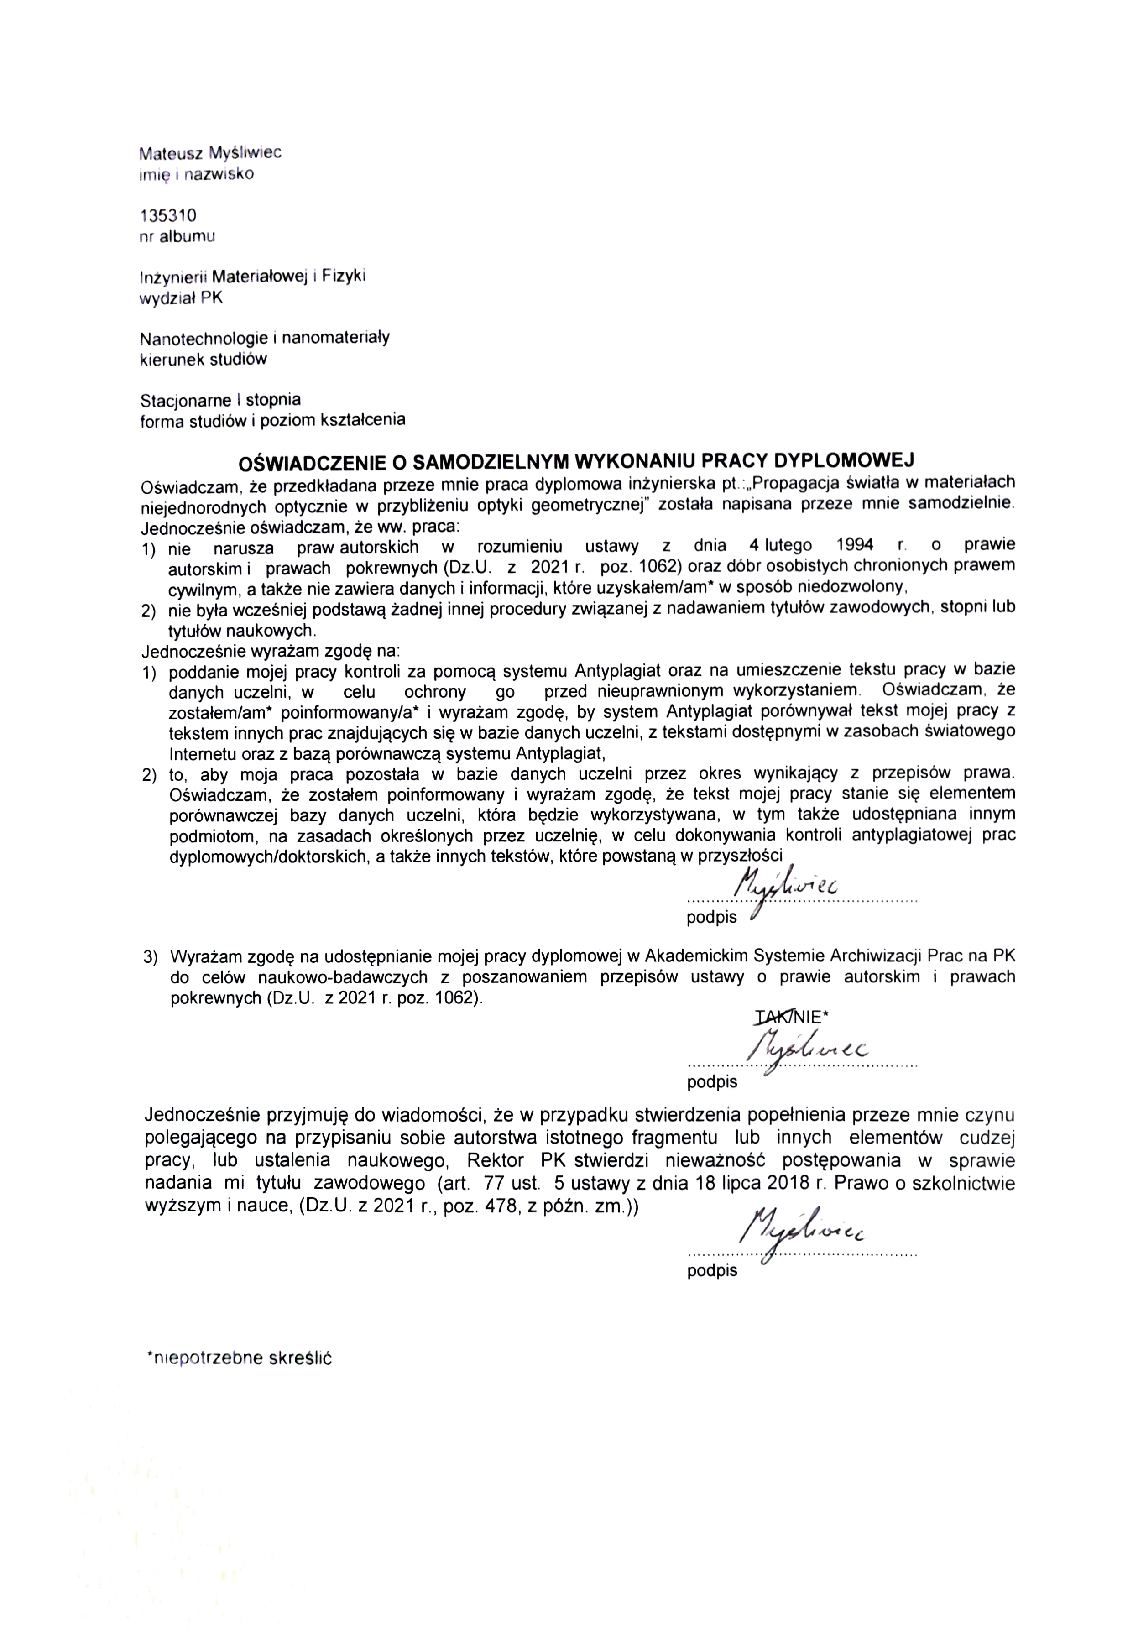
\includepdf[pages=-, scale=1.0, offset=.45in -1.0in]{frontpage/Oswiadczenie_podpisane.pdf}
\newpage
\thispagestyle{empty}
\begin{center}
{\bf Streszczenie}
\end{center}
Optyka geometryczna jest teorią opierającą się na rozprzestrzenianiu się światła w postaci promieni, wyjaśniającą powstawanie obrazów po odbiciu bądź załamaniu na ośrodkach optycznych. W~pracy jest wyjaśnione w jaki sposób opisywane jest światło w oparciu o równanie falowe uzyskane z rozważań Maxwella, a następnie równanie eikonału prowadzące w granicy wysokich częstości do zasady Fermata rozchodzenia się promieni. Jednak niejednorodność optyczna jest szerokim pojęciem obejmującym nie tylko samo rozpraszanie promieni świetlnych w ośrodkach, ale także odbijanie oraz załamywanie ich torów, co skutkuje zmianą kierunku promienia pod wpływem gradientu współczynnika załamania.  Rozwiązania zredukowanego układu równań różniczkowych promienia świetlnego wynikających z zasady wariacyjnej Fermata można uzyskać przy pomocy integratora opartego o metodę Rungego-Kutty w specjalnie napisanym do tego celu programie. Przy pomocy tego programu można wyznaczyć trajektorię promieni w zamodelowanych układach optycznych np.: w soczewce wypukłej lub wklęsłej, w układach złożonych z różnych typów ośrodków, w światłowodach itp. Uwzględniając dodatkowo prawo Cauchy’ego opisujące w dobrym przybliżeniu dyspersję współczynnika załamania w zależności od długości fali promienia optycznego, otrzymujemy kompletne narzędzie pozwalające badać propagację światła w ośrodku niejednorodnym. Wyjaśnienie działania programu do symulacji rozprzestrzeniania się promieni świetlnych oraz  pokazanie jego działania na różnych zaprogramowanych przykładach stanowi główną część pracy.\\
Słowa kluczowe: przybliżenie optyki geometrycznej, zagadnienia wariacyjne, metody Rugego-Kutty, propagacja światła

\begin{center}
{\bf Abstract}
\end{center}
Geometrical optics is a theory based on the propagation of light in the form of rays, explaining the formation of images after reflection or refraction in optical media. In this diploma thesis, it is explained how light is described based on the wave equation derived from Maxwell's considerations and then the resulting eikonal equation leading in the high frequency limit to Fermat's principle. However, optical inhomogeneity is a broad concept encompassing not only the mere scattering of light rays in media, but also the reflection and refraction of their paths, resulting in a change of ray direction under the influence of the  gradient of the refractive index.  Solutions of the reduced system of differential equations of a light ray resulting from the Fermat variational principle can be obtained with the use of a numerical integrator based on the Runge-Kutta method implemented in a program written for this purpose. With the help of this program it is possible to determine the trajectory of rays in the modelled optical systems, e.g.: passing through a convex or concave lens, moving in systems composed of different types of media, in optical fibres, etc. Additionally, taking into account the Cauchy law describing to a good approximation the dispersion of the refractive index depending on the wavelength of the optical ray, we obtain a complete tool allowing us to study the propagation of light in an inhomogeneous medium. The explanation of how the program for the simulation of the propagation of light rays works and the presentation of the results obtained for various programmed examples is the main part of this diploma thesis.\\
Keywords: geometrical optics approximation, variational problems, Ruge-Kutta methods, the propagation
of light
\newpage
\pagenumbering{Roman}
\tableofcontents

\newpage
\pagenumbering{arabic}

\chapter{Wstęp i cel pracy}

\quad \quad Przybliżenie optyki geometrycznej jest metodą do śledzenia toru promieni świetlnych w~celu projektowania układów zwierciadeł, pryzmatów i soczewek z jednolitych elementów optycznych. W~ciągu ostatnich kilkudziesięciu lat, prowadzone są badania nad rozchodzeniem się sygnałów w~ruchomych ośrodkach. Przyczyniły się do tego z jednej strony zastosowania układów elektromagnetycznych na coraz mniejszych długościach fal, a z drugiej strony nowe elementy optyczne:~takie jak światłowody i zintegrowane elementy optyczne. Zakres optyki geometrycznej obejmuje obecnie takie pojęcia, jak optyka w~dużych rozmiarach, optyka geodezyjna oraz optyka ośrodków niejednorodnych. Wprowadzenie do tej dziedziny teorii pola elektromagnetycznego uzupełnia ją o takie efekty jak dyfrakcja, fale akustyczne oraz fale ewanescencyjne (zanikające,~powstałe w~wyniku odbicia na granicy ośrodków o różnych współczynników załamania,~która zanika ekspotencjalnie zależnie od pokonanej odległości). Procesy optyczne wprowadziły z~kolei pewne nowe twierdzenia geometryczne oraz metody, które mają zastosowanie w~całej nauce optyki geometrycznej.

Celem pracy jest przedstawienie zagadnień wariacyjnych w~ośrodkach niejednorodnych op\-ty\-cznie, wyprowadzenie równań propagacji z odpowiedniej zasady Hamiltona, ponadto przedstawienie metody całkowania Bogackiego-Shampine'a RK3(2) z adaptowanym krokiem, która posłuży do poszukiwania torów promieni świetlnych w~układach optycznych z dyspersją współczynnika załamania.

\chapter{Materiały niejednorodne optycznie}

\indent Materiały optycznie niejednorodne to szeroka klasa materiałów. Odgrywają one ważną rolę w~wielu dziedzinach nauki. Poprzez medycynę \cite{huggins1999physics2000}, mikroelektronikę, \cite{debieu2013structural,bovard1990rugate,kusy1976structure}, energetykę słoneczną \cite{niklasson1985noble,smith1985surface}, komunikację \cite{huggins1999physics2000}, aż po przedmioty codziennego użytku, takie jak papier \cite{missori2004optical,missori2006modifications}. W~węższym sensie, ośrodek jest optycznie niejednorodny, gdy następuje zmiana kierunku promieni świetlnych pod wpływem gradientu współczynnika załamania. Zmiana funkcji die\-lek\-trycz\-nej -- jako skalara stałej dielektrycznej na odległościach, z założenia przekraczających długość fali światła propagującego się w~materiale, powoduje zakrzywianie się toru promieni świetlnych. 
Efekty związane z gradientami na mniejszej skali, porównywalnej z długością fali, wymagałyby opisu wykraczającego poza przybliżenie optyki geometrycznej. Ponadto, w~rozpatrywanym w~niniejszej pracy opisie przy pomocy jednego skalarnego współczynnika załamania, nie brane są pod uwagę efekty związane z anizotropią lokalnych własności materiału optycznego, kiedy w~każdym punkcie materiału wyróżnione są kierunki główne wielkości dielektrycznych, mających na ogół charakter tensorowy (analogiczna różnica dotyczy 
opisu naprężeń w~materiałach - w~przypadku materiałów izotropowych wystarczy posługiwać się pojęciem skalarnego ciśnienia,  a w~przypadku ogólniejszym, anizotropowym, należy odwołać się do pojęcia symetrycznego tensora naprężeń --- tensor taki zawiera informację o~trzech różnych skalarach -- odpowiednikach ciśnienia -- oraz informację o~orientacji w~przestrzeni trzech wzajemnie prostopadłych osi, którym te trzy skalary odpowiadają, opisując naprężenia wzdłuż tych kierunków). Pamiętając o~tym jakościowym rozróżnieniu pojęcia ośrodków niejednorodnych optycznie, poprzestaniemy na opisie biegu promieni optycznych odnosząc pojęcie niejednorodności do skalarnego współczynnika załamania,~który staje się funkcją zależną od punktu. 

Najprostszym przykładem materii niejednorodnej jest ziemska atmosfera. Przez zmienne temperatury oraz wysokości, na których jesteśmy, powietrze przybiera różne gęstości, co jest przyczyną zmiany gradientu współczynnika załamania światła. Kiedy światło opuszcza próżnię i~wchodzi do nowego ośrodka, jego prędkość ulega zmniejszeniu. Współczynnik załamania światła w~nowym ośrodku jest równy stosunkowi prędkości światła w~próżni do jego prędkości w~nowym ośrodku. Zmiany współczynnika załamania powietrza powodują, że światło pochodzące od Słońca i~gwiazd,~zwłaszcza gdy znajdują się one na horyzoncie, zakrzywia się przy wchodzeniu w~atmosferę. W~ten sposób gwiazda wydaje się wyższej na niebie niż jest w~rzeczywistości oraz nadal jest widoczna po tym jak znajdzie się pod horyzontem. Miraże czy fatamorgana powstają,~gdy nad terenem tworzą się gorące i~chłodne warstwy powietrza. Widzimy obrazy rzutowane wzdłuż linii prostych w~oparciu o~kierunek, w~którym promienie faktycznie wchodzą do oka \cite{katz2002introduction}. Z punktu widzenia obserwacji astronomicznych ważne są też przypadkowe zmiany współczynnika załamania wynikające z lokalnych zmian gęstości ośrodka na drodze promienia świetlnego. Pozorne nieuporządkowane migotanie gwiazd (ogólnie obiektów widzianych jako obiekty o~niewielkiej wielkości kątowej) i~towarzyszące mu nieuporządkowane zmiany barwy gwiazd lub ich położenia na sferze niebieskiej, to efekt owych lokalnych zmian współczynnika załamania.  

\section{W komunikacji i medycynie}
 \indent Odbicie wewnętrzne odgrywa kluczową rolę w~nowoczesnej komunikacji i~nowoczesnej medycynie poprzez światłowody. Światło jest przesyłane przez szklany pręt lub włókno tak, że padając na powierzchnię graniczną pod kątem większym niż kąt krytyczny, światło na swej drodze podlega ciągłemu całkowitemu odbiciu wzdłuż linii światłowodu bez strat związanych z odbiciem. Przy użyciu nowoczesnego szkła o~bardzo dużej przejrzystości, światłowód może przenosić sygnał świetlny bezstratnie na wiele kilometrów, bez wyraźnego tłumienia. Przyczyną, dla której skuteczniej jest używać światła w~włóknach szklanych niż elektronów w~drucie miedzianym do przesyłania sygnałów, jest to, że włókno szklane może przenosić informacje w~znacznie szybciej niż drut miedziany. Dzieje się tak dlatego, że impulsy laserowe podróżujące przez szkło,~mogą być włączane i~wyłączane znacznie szybciej niż impulsy elektryczne w~przewodzie. Praktyczne ograniczenie dla drutu miedzianego jest rzędu miliona impulsów lub bitów informacji na sekundę (co odpowiada szybkości transmisji jednego megabita na sekundę). Szybkość przesyłu informacji w~komercyjnych liniach telefonicznych jest zazwyczaj znacznie wolniejsza, niewiele przekraczając 30 do 50 tysięcy bitów informacji na sekundę (co odpowiada 30 do 50 baudów). Szybkość ta jest wystarczająca do prowadzenia rozmów telefonicznych lub przesyłania dokumentów do wydrukowania,~ale zdecydowanie zbyt wolna dla cyfrowych sygnałów telewizyjnych. Telewizja cyfrowa o~wysokiej rozdzielczości wymaga przesyłania informacji z szybkością około 3 milionów bitów lub impulsów co $3.3$ ms, co daje szybkość 90 milionów baudów. Kable światłowodowe są w~stanie przenosić impulsy lub bity w~tempie około miliarda na sekundę, a zatem dobrze nadają się do przesyłania zdjęć, utrzymania wielu rozmów telefonicznych jednocześnie czy telewizji cyfrowej. Łącząc wiele cienkich włókien razem, można przesłać kompletny obraz wzdłuż wiązki. Jeden koniec wiązki umieszcza się przy obserwowanym obiekcie, a jeśli włókna nie są pomieszane, obraz pojawia się na drugim końcu. Aby przekazać obraz o~wysokiej rozdzielczości, potrzebna jest wiązka około miliona włókien. Do wytworzenia takiej wiązki podgrzewa się dużą grupę małych włókien szklanych, aby zmiękczyć szkło, a następnie rozciąga się pęk, aż poszczególne pasma są bardzo cienkie. Jak wspomniałem, światłowody znajdują zastosowanie w~medycynie, a w~szczególności w~diagnostyce obrazowej. Robi się to za pomocą elastycznego instrumentu światłowodowego zwanego fiberoskopem. Operacja, taka jak usunięcie pęcherzyka żółciowego, która kiedyś wymagała otwarcia powłok brzusznych i~długiego okresu rekonwalescencji, może być teraz wykonana przez mały otwór w~pobliżu pępka oraz światłowodów do podglądu procedury \cite{huggins1999physics2000}.

\section{W elektronice}
\indent Materiały niejednorodne w~postaci cienkich warstw są wykorzystywane w~nowoczesnej mikroelektronice oraz przemyśle półprzewodników. Przykładem są warstwy wytworzone z niestechiometrycznego azotku krzemu \cite{debieu2013structural}. Ponadto w~przemyśle optycznym układy warstwowe składające się z cienkich warstw o~różnych współczynnikach załamania światła są czasami zastępowane przez odpowiednie niejednorodne cienkie warstwy. Jest to spowodowane lepszymi właściwościami optycznymi tych warstw w~porównaniu z układami warstwowymi, z powodu ich budowy w~szczególności chropowatości granic powierzchni. Przykładem takiej niejednorodnej cienkiej warstwy zastępującej układy warstwowe są filtry z gradientowym współczynnikiem załamania \cite{bovard1990rugate}. W układach mikroelektronicznych interesujące zastosowanie mają tak zwane grubowarstwowe rezystory cermetowe. Elementy te składają się z mieszaniny cząstek szkła i~przewodzących tlenków metali w~płynie organicznym. Najczęściej stosowanymi materiałami przewodzącymi są tlenki rutenu (RuO$_2$, Pb$_2$Ru$_2$O$_6$, Bi$_2$Ru$_2$O$_7$). Rezystory nakładane są metodą sitodruku, w~pożądany wzór, suszone i~wypalane (ogrzewanie do wysokiej temperatury). Grubość powstałych warstw wynosi zwykle 10-20 $\mu$m. Re\-zy\-sty\-wność warstw można zmieniać w~zakresie kilku rzędów wielkości poprzez zmianę ilości używanego tlenku metalu. Jest także zależne od temperatury, gdzie wykazuje minimum w~pobliżu temperatury pokojowej, co mówi o~niskim temperaturowym współczynniku rezystancji (TWR) \cite{kusy1976structure}.

\section{W energetyce słonecznej}
\indent Do efektywnego zbierania energii słonecznej niezbędne są powłoki selektywne, które charakteryzują się wysoką absorpcją energii słonecznej i~niską emisją termiczną. Stwierdzono, że bardzo dobrze nadają się do tego celu niejednorodne kompozyty metal-izolator. Współwystępujące kompozyty takie jak Ni-Al$_{2}$O, Pt-Al$_{2}$O$_{3}$, i~Co-Al$_{2}$O$_{3}$ \cite{niklasson1985noble}. Wydajność powłok można dodatkowo poprawić poprzez wykorzystanie chropowatości powierzchni. Dobrą selektywność wykazuje również kompozyt Mo-MoO$_{2}$, wytwarzany metodą chemicznego osadzania z fazy gazowej (czarny molibden). Inną komercyjną powłoką jest niklowy pigmentowany anodowy tlenek glinu wytwarzany metodą anodowania i~elektrolitycznego barwienia. W tych powłokach selektywna ab\-sor\-pcja cząstek metalu jest często wzmacniana przez inne efekty, takie jak interferencja i~tekstura powierzchni. Selektywne właściwości optyczne kompozytów metal-izolator mogą być w~dużym stopniu zrozumiane w~ramach teorii ośrodków \cite{smith1985surface}. Konieczne są dalsze badania w~celu uzyskania ilościowego zrozumienia właściwości optycznych kompozytów metal-izolator w~szerokim zakresie składu.

\section{Przykład materiału, o którym mało się mówi - papier}
\indent Arkusze papieru stanowią mało znany przykład materiałów, których właściwości optyczne są silnie regulowane przez efekty rozpraszania światła. Arkusze papieru składają się głównie z sieci włókien celulozy, których średnica waha się od około 1 do około 10 $\mu$m. Biały wygląd niezdegradowanego papieru wynika z jego efektu rozpraszania światła spowodowanego obecnością mniejszych składników ułożonych w~nieregularny sposób \cite{missori2004optical}. Papier jest materiałem o~dużym znaczeniu zarówno ze względu na jego zastosowania przemysłowe, jak i~wartość historyczną. Ma on ogromny wachlarz zastosowań, z których najbardziej powszechnym jest jako materiał do pisania. W dziedzinie przemysłu jest on również wykorzystywany jako izolator w~transformatorach elektrycznych dużej mocy. W czasach starożytnych papier otrzymywano z czystych włókien celulozowych bawełny, lnu lub konopii. Obecnie najczęściej otrzymuje się go z masy drzewnej. Papier może zawierać również dodatki, głównie środki usztywniające i~wypełniacze (takie jak skrobia, żelatyna, kalafonia, ałun, kreda), w~zależności od zastosowanej techniki produkcji. Celuloza jest liniowym homopolimerem złożonym z jednostek $\beta$-D-glukopiranozowy, połączonych ze sobą tworząc łańcuchy. Włókna powstają, ponieważ łańcuchy celulozy mają silną tendencję do agregacji w~wysoko uporządkowane jednostki strukturalne poprzez rozbudowaną sieć zarówno wewnątrz- jak i~międzycząsteczkowych wiązań wodorowych. W konsekwencji tworzy się układ hierarchiczny od pojedynczych łańcuchów aż do włókien. Podstawowe składniki supramolekularnej struktury celulozy obejmują zespół domen wysoko uporządkowanych (krystalicznych) oraz regionów nieuporządkowanych (amorficznych). Stopień degradacji papieru po pewnym czasie zależy od warunków środowiskowych, jakim został poddany. Wśród produktów utleniania, te które są odpowiedzialne za żółknięcie nazywane są chromoforami. Czysta celuloza nie absorbuje światła powyżej około 200 nm \cite{missori2006modifications}. Żółte zabarwienie widoczne w~starzejących się papierach wynika głównie z faktu, że chromofory w~papierze pochłaniają wyższe pasmo energetyczne światła widzialnego (odpowiadające fioletowi i~niebieskiemu) i~w~znacznym stopniu rozpraszają część żółtą i~czerwoną, dając w~ten sposób charakterystyczny żółto-brązowy odcień \cite{missori2004optical, missori2006modifications}.

\chapter{Przybliżenie optyki geometrycznej}

\indent Światło jest zjawiskiem elektromagnetycznym, a jego propagację można opisać za pomocą dwóch wzajemnie sprzężonych wektorów: pola elektrycznego i~magnetycznego. W praktyce wiele zjawisk można opisać używając tylko jednej z~tych dwóch wielkości wektorowych. Stąd takie uproszczenie prowadzi do teorii skalarnej, w~której światło traktowane jest jako funkcja skalarna, a powstała w~ten sposób teoria nosi nazwę optyki falowej. Gdy światło rozchodzi się wokół obiektów znacznie większych niż długość jego fali, falowa natura światła może się nie ujawnić i~jego rozchodzenie się można po prostu opisać za pomocą promieni, a odpowiadającą temu teorię nazywa się optyką geometryczną. Wszystkie te teorie są teoriami klasycznymi, ale istnieją inne zjawiska świetlne o~charakterze kwantowo-mechanicznym, których nie można wyjaśnić w~kategoriach klasycznej teorii elektromagnetycznej.

\section{Jednostki i notacja w pracy}

Oznaczenia wielkości użytych w pracy:
\begin{itemize}
\item Pęd cząstki $\vec{p},$
\item Funkcja Hamiltona $\cal H,$
\item Potencjał skalarny pola elektromagnetycznego $\varphi,$
\item Potencjał wektorowy pola elektromagnetycznego $\vec{A},$
\item Natężenie pola elektrycznego $\vec{E},$
\item Natężenie pola magnetycznego $\vec{H},$
\item Gęstość ładunku $\varrho,$
\item Gęstość prądu $\vec{j}.$
\end{itemize}
W pracy został użyty uproszczony zapis wektorów czterowymiarowych, czyli zespół czterech wielkości, który opisuje współrzędne zdarzenia $(ct,x,y,z)$. Jego kwadrat jest dany wyrażeniem:
%
$$(A^{0})^{2}-(A^{1})^{2}-(A^{2})^{2}-(A^{3})^{2}.$$
%
Do uproszenia zapisu wprowadzono dwa ,,rodzaje"~składowych tego wektora. Wielkość $A^i$ jest nazywany kontrawariantną składową, a $A_i$ - kowariantną składową czterowektora, a postać kwadratu czterowektora wygląda:
%
$$A^{i}A_{i}=A^{0}A_{0}+A^{1}A_{1}+A^{2}A_{2}+A^{3}A_{3}.$$
%
Opisany sposób oznaczania sumy wektorów czterowymiarowych, jest za pomocą, tzn. niemych wskaźników.

\section{Równanie falowe}


%\cmmt{jeśli już uznam ,że jakiś podrozdział został zakończony, wóczas wprowadzę niewielkie poprawki/uściślenia na bazie Pańskiego tekstu -- zmiany będą widoczne jak poniżej, ale wszystkie znikną w ostatecznej wersji przy pomocy redefinicji pewnych komend}
%\quad \quad 
%\cmmt{kwetię pierwszego wcięcia wprowadzanego tu komendą quad quad ustala sie globalnie a nie lokalnie w każdym przypadku}

\indent Pod nieobecność źródeł pola, równania Maxwella opisują pole elektromagnetyczne występujące w próżni, to znaczy, dla znikającej gęstości ładunku ($\varrho$=0) i znikających prądów ($\vec{j}=0$) otrzymujemy następujące równania
\begin{equation}
\begin{aligned}
&\rot{E}=-\frac{1}{c}\frac{\partial \vec{B}}{\partial t},&\quad   &\div{B}=0,&\\
&\rot{B}=\frac{1}{c}\frac{\partial \vec{E}}{\partial t},&\quad &\div{E}=0,&
\end{aligned}
\end{equation}
zwane próżniowymi równaniami Maxwella. Należy tu zaznaczyć, że w zagadnieniach pól e\-le\-ktro\-ma\-gne\-ty\-cznych w ośrodkach materialnych pojawiają się mikroskopowe źródła (jak ładunki,~prądy molekularne, dipole magnetyczne itd.) indukowane lub występujące na stałe w~materiale ośrodka, do opisu których wprowadza się wektory indukcji elektrycznej $\vec{D}$  i natężenia pola magnetycznego $\vec{H}$ (odpowiadających  wektorom polaryzacji oraz magnetyzacji ośrodka) powiązane z wektorem natężenia pola elektrycznego $\vec{E}$ i wektorem indukcji magnetycznej $\vec{B}$ od\-po\-wie\-dni\-mi równaniami materiałowymi, nawet gdy nie ma zewnętrznych prądów i ładunków. Ważnym wnioskiem z równań próżniowych jest to, że ich  
rozwiązania są różne od zera, co wskazuje na możliwość istnienia pól elektromagnetycznych w obszarach przestrzeni bez występowania ładunków. Pola tego rodzaju propagujące się w przestrzeni, muszą koniecznie być polami zmiennymi w czasie, ale i w obszarach próżni między ustalonymi źródłami mogą występować pola statyczne opisane funkcjami harmonicznymi, które też spełniają próżniowe równania Maxwella przy zadanych warunkach brzegowych.

Matematyczna struktura powyższych równań pozwala (w ujęciu przestrzennym z wyróźnionym czasem) opisać pola fizyczne $\vec{E}$ oraz $\vec{B}$ przy pomocy potencjału wektorowego $\vec{A}$ oraz funkcji skalarnej $\Phi$, kosztem pewnej niejednoznaczności związanej z symetrią cechowania elektromagnetyzmu.\footnote{W języku potencjałów istnieje jeszcze ujęcie relatywistyczne (tzn bez wyróżnionego czasu), w którym pola $\vec{A}$ oraz $\Phi$ wchodzą w skład potencjału czterowektorowego $A_{\mu}$.}
W tym ujęciu, do wyznaczenia równania falowego wystarczy określenie potencjału wektorowego fal elektromagnetycznych założywszy warunek dodatkowy $\Phi=0$. Wówczas
%
$$\vec{E}=-\frac{1}{c}\frac{\partial \vec{A}}{\partial t},\qquad \vec{B}=\rot{A}.$$    
%
Podstawiając wyrażenia do pierwszego opisanego równania Maxwella, otrzymujemy
%
$$\rot{\br{\rot{A}}}=-\Delta\vec{A}+ \grad{\br{\div{A}}}=-\frac{1}{c^2}\frac{\partial^2 \vec{A}}{\partial t^2}.$$
%
Następnie, ujednoznacznienie potencjału wektorowego $\vec{A}$ osiągamy w odpowiednim cechowaniu,~dodając do $\vec{A}$ niego gradient pewnej funkcji niezależnej od czasu (bez zmiany $\Phi$).  W szczególności, potencjał fali elektromagnetycznej można tak wybrać, aby
%
$$\div{A}=0.$$
%
Podstawiając wektor natężenia pola elektrycznego z do jego gradientu przyrównywanego do zera,~mamy
%
$$\div{}\!\br{\!\frac{\partial \vec{A}}{\partial t}\!}=\frac{\partial}{\partial t}\br{\div{A}}=0,$$
%
czyli gradient potencjału pola elektromagnetycznego jest funkcją samych tylko współrzędnych. Równanie falowe przybiera postać:
%
$$\Delta\vec{A}-\frac{1}{c^2}\frac{\partial^2 \vec{A}}{\partial t^2}=0.$$
%
Jest to właśnie równanie określające potencjały fal elektromagnetycznych \cite{TeoriaPolaLifszyc}.


\section{Powierzchnia falowe}

\quad \quad 
Szczególny przypadek fal elektromagnetycznych, w których pole zależy tylko od jednej współrzędnej, są fale płaskie. W przypadku tym równania pola przybierają postać:
%
$$\frac{\partial^2 f}{\partial t^2}-c^2 \frac{\partial^2 f}{\partial x^2}=0.$$
%
Cechą fali płaskiej jest to, że kierunek jej rozchodzenia się oraz amplituda są wszędzie jednakowe. Własności tych oczywiście nie ma dowolna fal elektromagnetyczna. Często jednak dowolne fale elektromagnetyczne, niebędące falami płaskimi, można w małych obszarach przestrzeni uważać za fale płaskie. Ujęcie takie jest słuszne jedynie wtedy, gdy wzdłuż odległości rzędu długości fali amplituda i kierunek rozchodzenia się fali prawie się nie zmieniają. Jeśli warunek jest spełniony, można mówić o powierzchni falowej, to znaczy powierzchni, na której we wszystkich punktach faza fali jest jednakowa. Powierzchnia falowa jest oczywiście płaszczyzną prostopadłą do kierunku jej rozchodzenia się. W każdym, niezbyt dużym, obszarze przestrzeni można uważać, że kierunek normalny do powierzchni falowej jest kierunkiem rozchodzenia się fali. Można wprowadzić przy tym pojęcie promieni – krzywe, których styczne w każdym punkcie pokrywają się z kierunkiem rozchodzenia się fali \cite{TeoriaPolaLifszyc}.

\section{Równanie eikonału}

Dla płaskiej fali monochromatycznej funkcja ma postać:
%
\begin{equation}\label{eq:eikonal}f=ae^{i(\sprod{k}{r}-\omega t + \alpha)}=ae^{i\psi}.\end{equation}
%
Gdy fala nie jest płaska i $\lambda \rightarrow 0$, amplituda $a$ jest funkcją współrzędnych i czasu, a faza,~zwana także eikonałem, nie ma tak prostej postaci jak we wzorze \ref{eq:eikonal}. W małych obszarach przestrzeni i małych przedziałach czasu eikonał można rozwinąć w szereg z dokładnością do wyrazów pierwszego rzędu \cite{TeoriaPolaLifszyc}:
%
$$\psi=\psi_{0}+\sprod{\vec{r}}{\frac{\partial \psi}{\partial \vec{r}}}+t\frac{\partial \psi}{\partial t}.$$
%
Porównując do równania fali monochromatycznej dostajemy:
%
$$\vec{k}=\frac{\partial \psi}{\partial \vec{r}}\equiv \grad{\psi},\qquad \omega=-\frac{\partial \psi}{\partial t},$$
%
co mówi nam, że falę w każdym małym obszarze przestrzeni można postrzegać jako falę płaską. W postaci czterowymiarowej równania można zapisać jako:
%
$$k_{i}=-\frac{\partial \psi}{\partial x^{i}}.$$
%
Otrzymujemy równanie eikonału, z związku $k_{i}k^{i}=0$:
$$\frac{\partial \psi}{\partial x_{i}}\frac{\partial \psi}{\partial x^{i}}=0$$.


\section{Zasada Fermata}

\indent Z postaci równania eikonału występuje zależność, ruch cząstki określony jest za pomocą równania Hamiltona-Jacobiego.
Funkcja działania $S(q,t)$ względem czasu jest związana z funkcją Hamiltona zależnością \cite{TeoriaPolaLifszyc}:
$$\frac{\partial S}{\partial t}+{\cal H}\!\br{q,p,t}=0.$$
A jej pochodne cząstkowe względem współrzędnych są równe pędom
%\cmmt{w poniższym równaniu Jacobiego nawias koniecznie musi byc większy -- pamiętać o tym w każdym podobnym przypadku}
%
%\cmmt{Równania to też część zdania -- należy stawiać kropki gdzie trzeba}
%
$$\frac{\partial S}{\partial t}+{\cal H}\!\br{q_{1},...,q_{s};\frac{\partial S}{\partial q_{1}},...,\frac{\partial S}{\partial q_{s}};t}=0.$$
%
Jest to równanie różniczkowe cząstkowe pierwszego rzędu drugiego stopnia, równanie Hamiltona-Jacobiego.
%\cmmt{wszędzie za instrukcją {\it end{equation}} wyrzucić znak nowej linii \verb"\\" bardzo to niedobrze wygląda -- zbyt duże odstępy }
%
W naszym przypadku zapisujemy działanie S to w postaci związków:
%
$$\vec{p}=\frac{\partial S}{\partial \vec{r}},\qquad H=-\frac{\partial S}{\partial t}.$$
%
Dla cząstki słuszne są równania Hamiltona :
%
$$\dot{\vec{p}}=-\frac{\partial {\cal H}}{\partial \vec{r}},\qquad \vec{v}=\dot{\vec{r}}=\frac{\partial {\cal H}}{\partial \vec{p}}.$$
%

\noindent Biorąc pod uwagę falę będącą superpozycją fal monochromatycznych o częstościach zmieniających się w pewnym niedużym przedziale i zajmujących pewien skończony obszar przestrzeni,~pęd i energia paczki falowej przekształcają się przy zmianie układu odniesienia odpowiednio jak wektor falowy i częstość. Można ustalić analogiczną zasadę w przypadku optyki geometrycznej do zasady najmniejszego działania w mechanice. Zastępując funkcję Hamiltona częstością, a pęd wektorem falowym $\vec{k}$, mogliśmy za funkcję Langrange’a w optyce geometrycznej przyjąć wyrażenie $\sprod{\vec{k}}{\frac{\partial \omega}{\partial \vec{k}}}-\omega$. Jednak wyrażenie będzie równe zero, niemożliwość wprowadzenia funkcji Langrange’a dla promieni wynika również bezpośrednio stąd, że rozchodzenie się promieni jest analogiczne do ruchu cząstek z masą równą zeru. Jeśli fala ma określoną stałą częstość $\omega$, to zależność jej pola od czasu określona jest mnożnik postaci $e^{-i\omega t}$. Dlatego dla eikonału takiej fali możemy przyjąć:
%
$$\psi=-\omega t + \psi_{0}\!\br{x,y,z},$$
%
gdzie $\psi_{0}$ jest funkcją samych współrzędnych. Równanie eikonału przebiera teraz postać:
%
$$\!\br{\grad{\psi_{0}}}^{2}=\frac{\omega^{2}}{c^2}.$$
%
Promienie w każdym punkcie powierzchni falowej, która jest powierzchnia stałego eikonału,~w~każdym punkcie są określone przez gradient $\nabla \psi_{0}$. Całkowanie przebiega po torze cząstki pomiędzy dwoma punktami, gdzie zakłada się pęd jako funkcję energii i współrzędnych cząstek. Dla promieni jest opisana zasada Fermata:
%
$$\delta \psi=\delta \int\!\! \sprod{\vec{k}}{d\vec{l}}=0.$$
%
W próżni $\vec{k}=\frac{\omega}{c}\vec{n}$, gdzie $\vec{n}$ jest wektorem jednostkowym kierunkiem prostopadłym do powierzchni stałej fazy (opisujący kierunek rozchodzenia się fali), otrzymujemy $(\sprod{\vec{n}}{d\vec{l}}=dl)$:
%
$$\delta \int\!\! dl = 0,$$
%
co odpowiada prostoliniowemu rozchodzeniu się promieni.


\chapter{Zagadnienie wariacyjne Fermata w ośrodku niejednorodnym}

\indent Rachunek wariacyjny jest ważny w~wielu problemach optymalizacyjnych i~naukach obliczeniowych, zwłaszcza w~formułowaniu metod elementów skończonych. Rachunek wariacyjny zajmuje się wyznaczaniem wartości stacjonarnych funkcjonału (z~reguły minimalnej jego wartości). 
Funkcjonał można zdefiniować jako funkcję kilku innych funkcji. Stąd rachunek wariacyjny może być stosowany do rozwiązywania problemów związanych z~optymalizacją trajektorii. Sam początek rozwoju tego zagadnienia zaczął się od definiowania przez Newtona zasad dynamiki,~wraz z~wprowadzeniem problemu brachistochronego przez J. Bernoulliego \cite{elsgolc2012calculus}, by później ważny wkład wnieśli Euler, Lagrange, d’Alembert i~Hamilton \cite{dacorogna2014introduction,goldstine2012history,giaquinta2013calculus}. Rachunek wariacyjny jest potężną metodą rozwiązywania problemów w~wielu dziedzinach nauki i~techniki, takich jak statyka i~dynamika ciał sztywnych, ogólna sprężystość, drgania, optyka, przede wszystkim stanowi fundament konstrukcji modeli fizycznych rzeczywistości.

\section{Ogólne zagadnienie wariacyjne. Równanie\\ Lagrange'a--Eulera}

\begin{figure}[htb]
    \centering
    \includegraphics[width=0.75\textwidth,trim={0 1.5cm 0 1.5cm},clip]{grafika/Rys1.jpg}
    \caption{\label{fig:Minimalizacja} Krzywe ilustrujące rozwiązanie dla różnych problemów minimalizacji, (1) minimalizacja drogi, (2) minimalizacja energii, (3) minimalizacja czasu, (4) znalezienie ekstremum funkcjonału}
\end{figure}
\indent Do zrozumienia ogólnego znaczenia zagadnienia wariacyjnego zostaną przedstawione problemy związane z minimalizacją, zaczynając od przypadku {\bf A}, minimalizacji ścieżki. Załóżmy, że mamy dwa punkty, które nazywamy $A(x_1,y_1)$ i $B(x_2,y_2)$. Jeśli spróbujemy zminimalizować odległość,~czyli znaleźć najkrótszą drogę łączącą nasze dwa punkty to wyrysujemy prostą linię,~która przybiera postać jak krzywa (1) na rysunku \figref{fig:Minimalizacja}. Długość te krzywej jest wyznaczana przez całkę
%
$$D = \int\limits_{x_1}^{x_2}\!\! \ud{s}.$$
%
\newpage
Z twierdzenia Pitagorasa:
%
$$\ud{s}^2 = \ud{x}^2 + \ud{y}^2 = \ud{x}^2 \sq{1+\!\left(\frac{\ud{y}}{\ud{x}}\right)^{\!\!2}}\quad \Rightarrow\quad \ud{s} = \sqrt{1+y'^2} \ud{x},$$ gdzie $y':= \frac{\ud{y}}{\ud{x}}$, 
%
ostatecznie otrzymujemy:
%
$$\int\limits_{x_1}^{x_2}\!\!\ud{s} \equiv D[y]  = \int\limits_{x_1}^{x_2}\!\!\sqrt{1+y'^2} \ud{x}.$$
%

 \noindent {\bf B. Krzywa łańcuchowa.} Jako kolejny przykład zastosowania rachunku wariacyjnego analizujemy problem krzywej łańcuchowej. W jednorodnym polu grawitacyjnym o~wartości przyspieszenia grawitacyjnego $g$,~zawieszamy nierozciągliwy łańcuch jednorodny (o~stałej gęstości $\rho$) na dwóch końcach w punktach $A(x_1,y_1)$ i $B(x_2,y_2)$. Chcemy zminimalizować całkowitą energie potencjalną łańcucha,~która jest zobrazowana krzywą (2) na rysunku \figref{fig:Minimalizacja}. Fragment łańcucha o~długości $ds$ ma masę $dm = \rho ds$,~gdzie $\rho$ jest gęstością masy łańcucha. W wysokość y każdego takiego fragmentu łańcucha,~długość pomnożona przez jego masę i stałą grawitacyjną $g$ jest równa energii potencjalnej segmentu. Jeśli kształt łańcucha opisany jest funkcją $y(x)$,~to energia potencjalna łańcucha jest proporcjonalna do funkcji:
%
$$E_p[y]=\int\limits_{x_1}^{x_2}\!\!\rho y g\, \ud{s} = \rho g \int\limits_{x_1}^{x_2}y\sqrt{1+y'^2}\, \ud{x}.$$
%

\noindent {\bf C. Zagadnienie brachistochrony.} Problem brachistochrony opisuje minimalizację czasu zsuwania się obiektu ze stanu spoczynku wzdłuż krzywej. Za przykład weźmy piłkę,~którą toczymy po zboczu z punktu $B(x_2,y_2)$ do punktu $A(x_1,y_1)$. Znajdujemy minimalny czas,~w którym piłka pokona drogę od A do B,~przy założeniu,~że spada tylko pod wpływem grawitacji. Rzeczywista forma krzywej brachistrochronicznej jest najbardziej zbliżona do krzywej “skoku narciarskiego” pokazanej w postaci krzywej (3) na rysunku \figref{fig:Minimalizacja}. Prawie pionowy spadek na początku przyspiesza piłkę bardzo szybko,~dzięki czemu jest w stanie szybciej pokonać poziomą część odległości,~aż do uzyskania największej wartości prędkości. Zmniejszenie kąta początkowego zwiększa całkowity czas,~przez spadek prędkości piłki. Prędkość $\vec{V}$ toczącej się na początku piłki jest równy $\sqrt{2gy}$ przy założeniu,~że $A=(0,0)$,~czas potrzebny na pokonanie łuku $ds$,~po przebyciu pionowego odcinku drogi,~przy tej prędkości wynosi $\frac{ds}{\sqrt{2gy}}$. Całkowity czas stoczenia jest dany wzorem:
%
$$T[y] = \int\limits_{x_1}^{x_2}\!\frac{\sqrt{1+y'^2}}{V}\ud{x} = \sqrt{2g}\int\limits_{x_1}^{x_2}\!\frac{\sqrt{1+y'^2}}{\sqrt{y}}\ud{x}.$$
%

\noindent Lagrangian jest różnicą pomiędzy energią kinetyczną i potencjalną układu,~który przemieszczając się z jednego czasu do drugiego. Układ podąża drogą punktów stacjonarnych względem lagrangianu,~tzn. w dowolnym momencie podąża ścieżką minimalizującą funkcjonał działania (krzywa (4) na rysunku \figref{fig:Minimalizacja}) \cite{rojas2014straight}.
%
$$F[y] = \int\limits_{x_1}^{x_2}\!\!\mathcal{L}\sq{x,y,y'}\ud{x}.$$

Koncepcja rachunku zmienności polega na tym,~że próbujemy znaleźć drogę,~która minimalizuje funkcję,~jako że droga jest funkcją to finalnie próbujemy znaleźć funkcję,~która minimalizuje funkcję.
%
\begin{figure}[htb]
    \centering
    \includegraphics[width=0.75\textwidth,trim={0 3.5cm 0 1.5cm},clip]{grafika/Rys2.jpg}
    \caption{\label{fig:RównanieLE}Problem optymalizacji funkcjonału działania}
\end{figure}
%
$y(x)$ jest optymalną drogą z punktu $A(x_1,y_1)$ do $B(x_2,y_2)$. Rozważamy wszystkie drogi łączące oba punkty,~$\eta(x)$ jest dowolną funkcją właściwą,~a $\epsilon$ jest stałą,~którą parametryzujemy całą rodzinę możliwych krzywych,~które mogą być właściwym rozwiązaniem $\epsilon\eta(x)$.
%
\begin{equation}\label{eq:war1}\overline{y}(x)=y(x)+\epsilon\eta(x).\end{equation}
%
$\eta$ jest arbitralną odmianą $y(x)$, musi spełniać dwa warunki brzegowe:
%
$$\eta(x_1)=\eta(x_2)=0,$$
%
\begin{equation}\label{eq:war2}\overline{y}'(x)=y'(x)+\epsilon\eta'(x).\end{equation}
%
Każda z tych całek może być napisana jako funkcja funkcji ogólnych $x,y,y'$:
%
$$F=\int\limits_{x_1}^{x_2}\!\!f\sq{x,y(x),y'(x)}\ud{x}.$$
%
Jeśli ścieżka y jest optymalna i ekstremalna, to musi być punktem stacjonarnym, tzn. pochodną tej funkcji musi być zero:
%
$$\left.\frac{dF}{d\epsilon}\right|_{\epsilon=0}=\left.\frac{d}{d\epsilon}\right|_{\epsilon=0}\int\limits_{x_1}^{x_2}\!\!f\sq{x,\overline{y}(x),\overline{y}'(x)}\ud{x}=0$$
%
$$\Rightarrow \int\limits_{x_1}^{x_2}\!\!\left.\br{f\sq{x,\overline{y}(x),\overline{y}'(x)}}\right|_{\epsilon=0}\ud{x}=0.$$
%
$$\Rightarrow \int\limits_{x_1}^{x_2}\!\left.\left(\frac{\partial f}{\partial x} \frac{\partial x}{\partial \epsilon}+\frac{\partial f}{\partial \overline{y}}\frac{\partial \overline{y}}{\partial \epsilon}+\frac{\partial f}{\partial \overline{y}'}\frac{\partial \overline{y}'}{\partial \epsilon}\right)\right|_{\epsilon=0}\ud{x}=0.$$
%
Z równiania \ref{eq:war1} wyciągamy:
\begin{equation}\label{eq:upro1}
    \Rightarrow \frac{\partial \overline{y}}{\partial \epsilon}=\eta(x).
\end{equation}
Oraz z równania \ref{eq:war2}:
\begin{equation}\label{eq:upro2}
    \Rightarrow \frac{\partial \overline{y}'}{\partial \epsilon}=\eta '(x).
\end{equation}
Używamy wyprowadzeń \ref{eq:upro1}, \ref{eq:upro2} do dalszego rozwiązywania:
%
$$\int\limits_{x_1}^{x_2} \!\left.\left(\frac{\partial f}{\partial \overline{y}}\dot\eta+\frac{\partial f}{\partial \overline{y}'}\dot\eta '\right)\right|_{\epsilon=0}\ud{x}=0.$$
%
Aby dostać końcowe równanie musimy zastosować całkowanie przez części: 
%
$$\left.\int\limits_{a}^{b}\!\!u\ud{V}=Vu\right|_{a}^{b}-\int\limits_{a}^{b}\!\!V\ud{u}.$$
%
Wykorzystujemy fakt, że rozwiązanie zbliża się do dokładnego rozwiązania, gdy $\epsilon$ wyzeruje:
%
$$\epsilon=0 \Rightarrow \overline{y}\rightarrow y,\quad\overline{y}'=y',$$
%
$$\Rightarrow \left.\frac{\partial f}{\partial \overline{y}'}\eta\right|_{x_1}^{x^2}+\int\limits_{x_1}^{x_2}\!\left(\frac{\partial f}{\partial y}-\frac{\ud{}}{\ud{x}}\!\left(\frac{\partial f}{\partial y'}\right)\right)\eta \ud{x}=0.$$
%
Ponieważ $\eta$ jest arbitralne, wszystko musi być równe zeru.
%
$$\frac{\partial f}{\partial y}-\frac{\ud{}}{\ud{x}}\!\left(\frac{\partial f}{\partial y'}\right)=0.$$
%
Dostajemy wyprowadzone równanie Eulera-Lagrange’a \cite{gregoryundersen}. Wykorzystując powyższe równanie można znaleźć rozwiązania dla przedstawionych w tym rozdziale problemach. Rozwiązania dla poszczególnych problemów (z dokłądnością do przesunięć i wyboru stałych dowolnych) są odcinkami funkcji mających nastepującą postać:\\
Dla {\bf A} będzie w postaci funkcji liniowej:
$$y=ax+b.$$
Dla {\bf B} rozwiązaniem będzie cosinus hiperboliczny:
$$y =a \cosh(x/b).$$
Dla {\bf C} jest to równanie cykloidy:
$$x(\gamma)=\frac{1}{2}\frac{1}{2gC^2}(\gamma-\sin{\gamma}),$$
$$y(\gamma)=\frac{1}{2}\frac{1}{2gC^2}(1-\cos{\gamma}).$$

\section{Prawo Snelliusa, przykład analityczny}



%\cmmt{zmieniono odnośnik do rysunku, proszę zobaczyć w tym tex jak budować odnośnik do rysunku w komendzie figure, zrobic wszedzie analogicznie}

\indent Korzystając z zasady Fermata można wyznaczyć załamanie światła na granicy ośrodków. Rysunek \figref{fig:PrawoSneliusa} przedstawia przechodzenie promienia z punktu A znajdującego się w ośrodku $n_1$, który pada w punkcie P na płaską powierzchnię styku dwóch ośrodków o współczynnikach załamania $n_1$ i $n_2$. Promień padający generuje jeden promień odbity i promień załamany. W naszym przykładzie zajmujemy się promieniem załamanym, który przechodzi przez ośrodek $n_2$ do punktu B. Przedstawiamy jedno z dwóch realnych przypadków załamania promienia, jeśli warunki byłyby odwrotne, to znaczy promień przechodziłby z ośrodka o większym współczynniku załamania światła do ośrodka o mniejszym współczynniku, to kąta załamania $\beta$ byłby większy od kąta padania $\alpha$. Zasada najmniejszego czasu Fermata jest bezpośrednim problemem minimalizacji -- znajdujemy najkrótszy możliwy czas potrzebny na rozchodzenie się światła z jednego punktu do drugiego. Odległości od A do x oraz od x do B wynoszą odpowiednio \cite{gregschool}:

\begin{figure}[htb]
    \centering
    \includegraphics[width=0.75\textwidth]{grafika/Rys3.jpg}
    \caption{\label{fig:PrawoSneliusa} Prawo Snelliusa. Geometria dla załamania promienia na granicy ośrodków. Promień świetlny oznaczony żółtą strzałką pada w punkcie P na płaszczyznę styku dwóch ośrodków, generują promień odbicia (czerwona strzałka) oraz promień załamania (zielona strzałka). Pokazany na przykładzie ośrodków powierzchnia-woda, pierwszy ośrodek ma mniejszy współczynnik załamania niż drugi ośrodek.}
\end{figure}
%
$$L_{1}=\sqrt{h^{2}+x^{2}},\qquad L_{2}=\sqrt{b^{2}+\br{a-x}^{2}}.$$
%
Całkowity czas wynosi:
%
$$t=\frac{L_1}{V_1}+\frac{L_2}{V_2}=\frac{\sqrt{h^{2}+x^{2}}}{c}+\frac{\sqrt{b^{2}+\br{a-x}^{2}}}{c}=n_{1}\sqrt{h^{2}+x^{2}}+n_{2}\sqrt{b^{2}+\br{a-x}^{2}}.$$
%
Zminimalizujemy to wyrażenie, biorąc pochodną czasu względem położenia x i ustawiając wynik na zero:
%
$$\frac{dt}{dx}=\frac{1}{2}n_{1}\frac{2x}{\sqrt{h^{2}+x^{2}}}-\frac{1}{2}n_{2}\frac{2\br{a-x}^{2}}{\sqrt{b^{2}+\br{a-x}^{2}}}=0,$$
%
$$\Rightarrow n_{1}\frac{x}{\sqrt{h^{2}+x^{2}}}-n_{2}\frac{\br{a-x}}{\sqrt{b^{2}+\br{a-x}^{2}}}=0,$$
%
$$\Rightarrow n_{1}\cos\br{\pi /2-\alpha}-n_{2}\cos\br{\pi /2-\beta}.$$
Przekształcenie cosinusów daje prawo Sneliusa:
%
$$n_{1}\sin\alpha=n_{2}\sin\beta.$$

\newpage
\section{Wyprowadzenie zredukowanych równań promieni świe\-tlnych w ośrodku niejednorodnym. Przypadek trajektorii płaskich (beztorsyjnych)}
\indent Z poprzednich rozważań wynika, że zasada wariacyjna Fermata dla promienia świetlnego propagującego się po płaszczyźnie prowadzi do układu dynamicznego opisanego funkcją Lagrange'a:%
\begin{equation}\label{eq:lagrangian_ds}L=e^{\nu(x,y)}\sqrt{\dot{x}^{2}+\dot{y}^{2}}\,\ud{s}.\end{equation}
Płaszczyznę taką możemy zrealizować napylając warstwę doskonale odbijającą po obu stronach płaskiej folii o danym rozkładzie współczynnika załamania (granicę ośrodka może też tworzyć bardzo duży gradient współczynnika załamania w kierunku normalnym do płaszczyzny). W przypadku ogólnej powierzchni w przestrzeni, w powyższej funkcji należy w miejsce euklidesowego tensora metrycznego wprowadzić tensor metryczny indukowany na tej powierzchni.
%
Powyższy Lagrangian jest jednorodny stopnia $1$ względem prędkości,\footnote{Funkcja $f$ jest jednorodna stopnia $n$ względem swoich  argumentów $u^i$, jeżeli $f(\lambda u^i)=\lambda^n f(u^i)$, dla dowolnego rzeczywistego $\lambda\neq0$. Dla takiej funkcji zachodzi twierdzenie Eulera $u^i\partial_if=nf$.} zatem jest on reparametryzacyjnie inwariantny, to znaczy nie zależy od wyboru parametryzacji wzdłuż krzywej. W dalszej części zakładamy, że krzywą będziemy parametryzować długością łuku $s$ na płaszczyźnie euklidesowej\footnote{Rozdział przygotowany na podstawie materiałów do wykładu z~metod obliczeniowych dla studentów kierunku Fizyka Techniczna PK.}. 

\subsection{Interpretacja czasoprzestrzenna}
\indent Układ dynamiczny opisany Lagrangianem \eqref{eq:lagrangian_ds} można uważać za model cząstki swobodnej w~ dwuwymiarowej przestrzeni zakrzywionej\footnote{Każda rozmaitość dwuwymiarowa jest lokalnie konforemnie równoważna płaszczyźnie euklidesowej.} zdefiniowanej przez element łuku $\ud{l}$
\begin{equation}\label{eq:elem_lin}\ud{l}^2=e^{2\nu(x,y)}\br{\ud{x}^2+\ud{y}^2}.\end{equation} Wycałkowany element łuku $\ud{l}$ można traktować jako efektywną głębokość optyczną,~różną od faktycznej długości łuku $s$ toru promienia świetlnego. 
Na podstawie wcześniejszej interpretacji $\ud{l}=c\,\ud{t}$. Przepisując powyższy element liniowy do postaci
$$\ud{x}_{\mu}\ud{x}^{\mu}\equiv c^2\ud{t}^2-e^{2\nu(x,y)}\br{\ud{x}^2+\ud{y}^2},$$ dochodzimy do wniosku,~że promienie świetlne w~ośrodku niejednorodnym można zreinterpretować w~języku dynamiki cząstek zerowych (fotonów) w~zakrzywionej $1{+}2$ wymiarowej czasoprzestrzeni statycznej z~globalnym czasem $t$ i hiperpowierzchniami stałego czasu opisanymi metryką przestrzenną \eqref{eq:elem_lin}. Dla powyższej metryki krzywizna  Gaussa\footnote{W przyjętych tu konwencjach znaków $K$ odpowiada krzywiźnie Gaussa,~która dla sfery jednostkowej jest równa 1.} hiperpowierzchni stałego czasu jest równa
 $$K=-e^{2\nu(x,y)}\br{\frac{\partial^2\nu}{\partial{x}^2}+\frac{\partial^2\nu}{\partial{y}^2}}.$$ Nawiasem mówiąc,~krzywizna omawianej czasoprzestrzeni rozumiana jako skalar Ricciego byłaby dwa razy większa,~jednakże nie można takiej krzywizny rozumieć na sposób grawitacyjny,~gdyż w~grawitacji trójwymiarowej (po raz pierwszy badanej przez A. Staruszkieicza w~roku 1963) z~przyczyn strukturalnych nie mogą istnieć rozciągłe źródła pola grawitacyjnego a jedynie pun\-kto\-we,~a przestrzenie stałego czasu muszą być lokalnie płaskie \cite{AStar1963}. 
 
%\cmmt{Znaleźć takie $\nu$, by krzywizna $K$ była równa stałej $1/a^2$}
\subsection{Redukcja równań promienia świetlnego}
\indent Jak wcześniej zauważyliśmy,~omawiany model jest reparametryzacyjnie inwariantny. To oznacza,~że parametr niezależny można wybrać w~sposób dowolny.
W parametryzacji naturalnej (długością łuku $s$) prędkości nie są niezależne,~zachodzi następujący wiąz dla prędkości $$\dot{x}^2+\dot{y}^2=1.$$ Zatem składowe prędkości w~tej parametryzacji są jednocześnie kosinusami kierunkowymi jednostkowego wektora prędkości. W szczególności kierunek ten opisać można jednoznacznie przez podanie kąta $\varphi$ takiego,~że: $$\dot{y}=\sin{\varphi(s)}, \qquad \dot{x}=\cos\varphi(s).$$
%
%$$\left\{\begin{matrix}
% & \dot{y}=\sin{\varphi(s)} \\ 
% & \dot{x}=\cos\varphi(s)
%\end{matrix}\right.$$
%
%Parametryzacja kątem wektora stycznego:
%
%$$\frac{\dot{y}}{\dot{x}}=\tg{\varphi},$$
%
Dla Lagrangianu jednorodnego stopnia $1$ względem prędkości pędy kanoniczne również będą wyznaczone kątem $\varphi$: 
$$p_x\equiv\frac{\partial L}{\partial \dot{x}}=e^{\nu}\frac{\dot{x}}{\sqrt{\dot{x}^{2}+\dot{y}^{2}}}=e^{\nu}\cos\varphi,\qquad p_y\equiv\frac{\partial L}{\partial \dot{y}}=e^{\nu}\frac{\dot{y}}{\sqrt{\dot{x}^{2}+\dot{y}^{2}}}=e^{\nu}\sin\varphi.$$
Równania Lagrange'a-Eulera $\dot{p}_x=\partial_xL$ i $\dot{p}_y=\partial_yL$, po obustronnym podzieleniu przez $e^{\nu}$,~przyjmują nastepującą postać
$$e^{-\nu}\frac{d}{ds}\br{e^{\nu}\cos\varphi}=\nu_{,x}, \qquad e^{-\nu}\frac{d}{ds}\br{e^{\nu}\sin\varphi}=\nu_{,y}.$$
%$$\frac{d}{ds}\frac{L}{\partial\dot{x}}=\frac{\partial L}{\partial x}, \qquad %\frac{d}{ds}\frac{L}{\partial\dot{y}}=\frac{\partial L}{\partial y}.$$
Wykonując różniczkowanie $e^{-\nu}\ud{e^{\nu}}/{\ud{s}}$ oraz wykorzystując związek prędkości z~kątem $\varphi$ otrzymujemy $\nu_{,x}\cos\varphi+\nu_{,y}\sin\varphi$ skąd, po uporządkowaniu, wynikają
%$$\left\{\begin{matrix}
% & \br{\nu_{,x}\cos\varphi+\nu_{,y}\sin\varphi}\cos\varphi-%\dot{\varphi}\sin{\varphi}=\nu_{,x} \\ 
% & %\br{\nu_{,x}\cos\varphi+\nu_{,y}\sin\varphi}\sin\varphi+\dot{\varphi}\cos\varp%hi=\nu_{,y}
%\end{matrix}\right.$$
%Mnożymy oba równania przez $e^{-\nu}$,otrzymując:
dwa liniowo zależne równania
$$\left\{\begin{matrix}
 & -\nu_{,x}\sin^{2}{\varphi}+\nu_{,y}\sin\varphi\cos\varphi=\dot{\varphi}\sin{\varphi} \\ 
 & \nu_{,x}\sin\varphi\cos\varphi-\cos^{2}\nu_{,y}=-\dot{\varphi}\cos{\varphi}
\end{matrix}\right.$$
dające jedno niezależne równanie $\dot{\varphi}=-\nu_{,x}\sin{\varphi}+\nu_{,y}\cos{\varphi}$, które razem z~wyrażeniami na prędkości daje układ trzech równań pierwszego rzędu postaci
%
%$$\left\{\begin{matrix}
% & -\nu_{,x}\sin{\varphi}+\nu_{,y}\cos{\varphi}=\dot{\varphi} \\ 
% & -\nu_{,x}\sin\varphi+\nu_{,y}\cos\varphi =\dot{\varphi}
%\end{matrix}\right.$$
%
\begin{equation}\label{eq:zredukowany}
\left\{\begin{array}{l}
  \dot{x}=\cos{\varphi} \\ 
  \dot{y}=\sin{\varphi} \\
  \dot{\varphi}=\nu_{,y}\cos{\varphi}-\nu_{,x}\sin{\varphi}
\end{array}\right.
\end{equation}
Jest to poszukiwany zredukowany układ równań toru promienia świetlnego.

\subsection{Interpretacja geometryczna zredukowanych równań toru promienia świetlnego}
\indent Zauważmy, że $\nu_{,y}\cos{\varphi}-\nu_{,x}\sin{\varphi}=\br{\vprod{\dot{\vec{r}}}{\grad{\!\nu}}}_z$, to znaczy, $\dot{\varphi}$ zadane jest przez trzecią składową iloczynu wektorowego 
jednostkowego wektora prędkości i gradientu skalara $\nu$: $\dot{\varphi}=\br{\vprod{\dot{\vec{r}}}{\grad{\!\nu}}}_z$. Wynika stąd w~szczególności, że promień świetlny poruszający się w~kierunku gradientu współczynnika załamania (prostopadle do linii stałej wartości $\nu$), nie ulega ugięciu. Geometrycznie $\dot{\varphi}$ opisuje lokalną krzywiznę toru promienia świetlnego. Istotnie, oznaczając przez $\vec{t}$ jednostkowy wektor styczny
$\{\dot{x},\dot{y}\}$ mamy $\dot{\vec{t}}=\dot{\varphi}\vec{n}$, gdzie $\vec{n}\equiv\{-\sin{\varphi},\cos{\varphi}\}$ jest jednostkowym wektorem normalnym do krzywej. W geometrii różniczkowej krzywych dowodzi się, że w parametryzacji łukowej (naturalnej) wektory $\dot{\vec{t}}$ i $\vec{n}$ są proporcjonalne do siebie a współczynnikiem proporcjonalności jest skalar krzywizny krzywej oznaczany przez $\kappa$:  $\dot{\vec{t}}=\kappa \vec{n}$, stąd $\dot{\varphi}=\kappa$. Zatem prędkości $\dot{x}$ oraz $\dot{y}$ wyznaczają lokalny kierunek styczny do toru promienia świetlnego, natomiast ,,prędkość kątowa"  \, $\dot{\varphi}$ wyznacza lokalną krzywiznę tego toru. Oczywiście mamy tu wszędzie na myśli prędkości jako pochodne względem parametru naturalnego a nie względem czasu. By było dodatkowo możliwe śledzenie promienia w czasie, to układ równań  \eqref{eq:zredukowany} należy uzupełnić o następujące równanie
$$\dot{t}=c^{-1}e^{\nu}.$$

\section{Sprowadzenie układu równań ruchu drugiego rzędu do postaci kanonicznej $Y'(x)=F(x,Y(x))$}
\label{s:spro_ukl}

\indent
Każdy układ równań różniczkowych zwyczajnych, niezależnie od liczby takich równań oraz rzędu poszczególnych równań, można sprowadzić do ogólnej postaci układu dynamicznego $$Y'(x)=F(x,Y(x)),$$ gdzie $x$ jest zmienną niezależną (zazwyczaj czasem) a $Y(x)$ jest wektorem poszukiwanych zmiennych konfiguracyjnych. Funkcja wektorowa F przyporządkowuje każdej wartości $x$ wektor pochodny $Y'$ zależny od zmiennej niezależnej $x$ (na ogół od czasu $t$). $Y'(x)$ interpretujemy jako wektor prędkości poruszającego się punktu $Y(t)$, zatem powyższe równanie opisuje pewien ruch w abstrakcyjnej przestrzeni  stanów konfiguracji takiego układu. Każde rozwiązanie tego równania będzie ruchem odbywającym się pod wpływem pola $F$,~fun\-kcja wektorowa $F$ określa w tej przestrzeni ciągłe pole wektorowe (przy założeniu, że funkcja ta jest ciągła). 

Mając układ  równań różniczkowych zwyczajnych dowolnego rzędu, zawsze możemy go przekształcić do układu równań pierwszego rzędu przez wprowadzenie dodatkowych zmiennych niezależnych. W szczególności 
gdy rozwiązujemy układ mechaniczny złożony z zespołu $N$ cząstek w~przestrzeni fizycznej, których położenia opisane są równaniami Newtona drugiego rzędu,~można przepisać je do równoważnego układu 6N równań pierwszego rzędu. Na koniec otrzymujemy układ równań bezwymiarowych przez przekształcenia w takim sposób, aby wszystkie funkcję miały wspólny argument.

\subsection{Przykłady}

\subsubsection{Cząstka w jednorodnym polu elektrycznym i jednorodnym polu magnetycznym}
\indent Zakładamy, że pola $\vec{B}$ oraz $\vec{E}$ są jednorodne i wzajemnie równoległe (oba wektory są stałe w rozpatrywanym fragmencie przestrzeni i niezależne od czasu). Osie układu współrzędnych dobieramy tak, że $\vec{E}$ odpowiada kierunkowi wersora osi $z$. 
Wówczas równania ruchu dla cząstki o masie $m$ i ładunku elektrycznym $q$ w tym polu
$$m\ddot{\vec{r}}=q \vec{E}+q\dot{\vec{r}}\times\vec{B}$$ przybierają postać następujących $3$ liniowych równań różniczkowych zwyczajnych  drugiego rzędu
$$m\ddot{x}=q B \dot{y},\qquad
m\ddot{y}=-q B \dot{x}, \qquad
m\ddot{z}=q E.$$ %
Po wprowadzeniu prędkości $v_x\equiv\dot{x}$, $v_y\equiv\dot{y}$ oraz $v_z\equiv\dot{z}$, równania powyższe przybierają postać równoważną układowi $6$ liniowych równań różniczkowych zwyczajnych pierwszego rzędu
$$
\dot{v}_x=\frac{q B}{m} v_y,\qquad \dot{x}=v_x,\qquad
\dot{v}_y=-\frac{q B}{m} v_x,\qquad\dot{y}=v_y,\qquad
\dot{v}_z=\frac{q E}{m},\qquad\dot{z}=v_z.$$
Dalej, wprowadzając bezwymiarową zmienną fazową $\phi\equiv \frac{Bq}{m}t$ w miejsce czasu,  skalę długości $r_o=\frac{Em}{B^2q}$ oraz skalę prędkości $v_o=\frac{E}{B}$, otrzymuje się równowazny układ równań bezwymiarowych
$$\psi_1'=\psi_2,\qquad \psi_2'=-\psi_1,\qquad \psi_3'=1,\qquad \xi_1'=\psi_1,\qquad \xi_2'=\psi_2
,\qquad \xi_3'=\psi_3,$$ gdzie 
$x(t)\equiv r_o\,\xi_1(\phi)$, $v_x(t)\equiv v_o\,\psi_1(\phi)$,
$y(t)\equiv r_o\,\xi_2(\phi)$, $v_y(t)\equiv v_o\,\psi_2(\phi)$,
$z(t)\equiv r_o\,\xi_3(\phi)$, $v_z(t)\equiv v_o\,\psi_3(\phi)$, a argumentem wszystkich funkcji jest zmienna niezależna $\phi$. Wprowadzając teraz wektor $Y=[\xi_1,\xi_2,\xi_3,\psi_1,\psi_2,\psi_3]$, odwzorowanie $F$ odpowiadające rozważanemu zagadnieniu ruchu zadane jest układem liniowym 
$$\left[\begin{array}{c}
y'_1\\y'_2\\y'_3\\y'_4\\y'_5\\y'_6\end{array}\right]=
F(\phi,Y)\equiv\left[\begin{array}{cccccc}
0 & 0 & 0 & 1 & 0 & 0\\
0 & 0 & 0 & 0 & 1 & 0\\
0 & 0 & 0 & 0 & 0 & 1\\
0 & 0 & 0 & 0 & 1 & 0\\
0 & 0 & 0 & -1 & 0 & 0\\
0 & 0 & 0 & 0 & 0 & 0\\
\end{array}\right]\cdot \left[\begin{array}{c}
y_1\\y_2\\y_3\\y_4\\y_5\\y_6\end{array}\right]+\left[\begin{array}{c}
0\\0\\0\\0\\0\\1\end{array}\right] .$$

\subsubsection{Odwzorowanie $F(\chi,Y)$ odpowiadające zredukowanym równaniom toru promienia świetlnego}
W poprzednich rozważaniach uzyskaliśmy układ zredukowanych równań toru ruchu promienia świetlengo:
$$
\left\{\begin{array}{l}
  \dot{x}=\cos{\varphi} \\ 
  \dot{y}=\sin{\varphi} \\
  \dot{\varphi}=\nu_{,y}\cos{\varphi}-\nu_{,x}\sin{\varphi}
\end{array}\right.
$$
Dodatkowo, aby móc analizować krzywą promienia, do powyższego układu równań wprowadzamy zmienną czasową $t$ będącą funkcją długości łuku $s$ i zdefiniowaną według wzoru:
$$t-t_0=\int\limits_{s_0}^{s_1}\!\! \frac{ds}{v}=\int\limits_{s_0}^{s_1}\!\! \frac{ds}{c}n,$$
z skąd wynika równanie różniczkowe:
$$\dot{t}=\frac{dt}{ds}=\frac{n}{c},$$
gdzie $t_0$ jest chwilą początkową odpowiadającą parametrowi $s_0$.
Przyjmując bezwymiarową zmienną czasową $\tau=c t$ otrzymujemy dodatkowe równanie postaci:
$$\tau=\frac{\ud{\tau}}{\ud{s}}=n(x,y)=e^{\nu(x,y)}.$$
Aby skonstruować odpowiadające temu układowi równań różniczkowych odwzorowanie $F(\chi,Y(\chi))$,~przyjmujemy nastepujące pryporządkowania: $s\to \chi$, $x \to y_1$, $y \to y_2$, $\phi \to y_3$, $\tau \to y_4$, skąd $\dot{x} \to y'_1$, $\dot{y} \to y'_2$, $\dot{\varphi} \to y'_3$,  $\dot{\tau} \to y'_4$:\\
$$\begin{matrix}
F(\chi,Y)=F(s,y'_1,y'_2,y'_3,y'_4)=(cos(y_3),~sin(y_3),\\ 
\nu_{,y}(y_1,y_2)cos(y_3)-\nu_{,x}(y_1,y_2)sin(y_3),~e^{\nu(y_1,y_2).})
\end{matrix}$$


\chapter{Wyprowadzenie formuły metody Rungego-Kutty drugiego i trzeciego rzędu. Metoda całkowania Bogackiego-Shampiege'a RK3(2) z adaptowanym krokiem}

\indent Problemy, które można było rozwiązać, stały się poważniejsze i~bardziej złożone, automatyczne monitorowanie błędów i~kontrola wielkości kroku stały się nie tylko potrzebne, ale wręcz konieczne. Postęp w~dziedzinie metod Runge-Kutta oraz główny cel używania tych metod, czyli do produkcji wydajnego i~niezawodnego programu do analizy równań różniczkowych, stał się czynnikiem napędzającym prace badawcze. Oprócz zastosowania metod Runge-Kutta w~ich tradycyjnej roli rozwiązujących równania różniczkowe, podobne rodzaje problemów wartości początkowej są możliwe do rozwiązania metodami odpowiednio dostosowanymi do bardziej ogólnej klasy problemów. Przykładami tych problemów są cząstkowe równania różniczkowe, całki Volterry,~równania różniczkowo-algebraiczne i~stochastyczne równania różniczkowe. Krótko mówiąc,~badania nad metodami Runge-Kutta są ważnym przedsięwzięciem, ponieważ angażują pracę badaczy w~wielu dziedzin: matematyki, informatyki, chemii, fizyki.

Metoda Bogackiego-Shampine’a jest bardziej wydajną oraz ma lepszą stabilność aniżeli inne tego typu metody (np. Dormand-Prince’a, Fehlberga). Opartą ją na trójstopniowej formule trzeciego rzędu Ralstona, ze względu na najlepszą stabilność. Ponadto, dodano automatyczną kontrolę wielkości kroku za pomocą metody drugiego rzędu, co wiąże się z niewielkim kosztem na krok. Nie tylko kontrola zwraca się poprzez zapewnienie najbardziej efektywnego rozmiaru kroku, ale także unika rozmiarów kroków, które prowadzą do niestabilności.

Do utrzymania niskich kosztów na krok, ograniczono się do minimalnej liczby etapów. Przy doborze parametrów sugerowano się, aby były w pewnym sensie małe, tak aby mieć formułę dokładną dla ,,typowego"~problemu \cite{bogacki19893}. Najlepszą możliwością jest uczynienie niektórych z~tych współczynników zerowymi, ponieważ wtedy dla niektórych problemów wzór będzie rzędu 3,~co można było uzyskać przy pomocy wzorów przedstawionych przez Ralstona \cite{ralston1962runge}:
$$k_{1}=h_{n}f\br{x_{n},y_{n}},$$
$$k_{2}=h_{n}f\br{x_{n}+\alpha h_{n},y_{n}+ A \alpha k_1},$$
$$k_{3}=h_{n}f\br{x_{n}+\beta h_{n},y_{n}+ B \gamma  k_{1} + B (\beta - \gamma) k_{2}},$$
\begin{equation}\label{eq:RK3}
y_{n+1}-y_{n}=w_{1} k_{1}+w_{2} k_{2}+(1 - w_{1} -w_{2}) k_{3}.
\end{equation}
Po wyznaczeniu parametrów dowolnych, zakładając $A=1, \quad B=1$, formuła będzie wyglądała następująco:
$$k_{1}=h_{n}f\br{x_{n},y_{n}},$$
$$k_{2}=h_{n}f\br{x_{n}+(\frac{1}{2})h_{n},y_{n}+\frac{1}{2}k_1},$$
$$k_{3}=h_{n}f\br{x_{n}+(\frac{3}{4})h_{n},y_{n}+(\frac{3}{4})k_{2}},$$
$$y_{n+1}-y_{n}=(\frac{2}{9})k_{1}+(\frac{1}{3})k_{2}+(\frac{4}{9})k_{3}.$$
Wzór ten nie do końca minimalizuje normę euklidesową współczynników błędu obcięcia, ale różnica jest zbyt mała, aby miała jakiekolwiek znaczenie praktyczne.

\section{Metoda Bogackiego-Shampine'a RK3(2)}\label{s:A}
\indent Wykorzystano dwustopniowe wzory RK, aby ponownie wykorzystać etapy powstałe w ocenie formuły rzędu trzeciego, aby otrzymać wynik $y_{n+1}$ rzędu drugiego. Wszystkie wzory drugiego rzędu Rungego - Kutta mają ten sam obszar stabilności, podobnie jak wszystkie trzystopniowe wzory trzeciego rzędu. W przypadku dwustopniowego istnieje niewielka elastyczność w zakresie uzyskania wysokiej jakości oszacowania błędu. Dodatkową elastyczność uzyskuje się poprzez uświadomienie sobie, że większość kroków kończy się sukcesem, a jeśli krok jest sukcesem, pierwszym etapem następnego kroku jest zawsze $f(x_{n+1},\hat{y}_{n+1})$. Poprzez dodanie etapu 
$$k_{4}=f\br{x_{n}+h,\hat{y}_{n}+h\sum_{j=1}^{3}\hat{b}_{j}k_{i}},$$
i rozważenie formuły drugiego rzędu w postaci:
$$y_{n+1}=\hat{y}_{n}+h\sum_{i=1}^{4}b_{i}k_{i},$$
uzyskuje się elastyczność przy bardzo niewielkim dodatkowym koszcie. To podejście jest nazywane FSAL, First Same As Last. W tym podejściu określamy, która z pary formuł zostanie użyta do posunięcia kroku naprzód, czyli lokalną ekstrapolacje \cite{bogacki19893}. 

Opracowanie formuły Bogackiego-Shampine'a RK3(2) przy pomocy narzędzi komputerowej algebry komputerowej Mathematica\footnote{Przygotowany na podstawie materiałów do wykładu z metod obliczeniowych dla studentów kierunku
Fizyka Techniczna PK}. Pracujemy na formule trzeciego rzędu Ralstona, ale żeby zmniejszyć do minimum błąd metody oraz użyć później tego parametru do kontroli kroku przy całkowaniu toru ruchu promienia świetlnego używamy go wraz z formułą drugiego rzędu. Parametry do formuły trzeciego rzędu uzyskaliśmy przyjmując założenia:
\begin{enumerate}
\item symetria przyrostów punktów węzłowych, tzn, jeśli x$\rightarrow$ x + A $\Delta$x to y$\rightarrow$ y + A $\Delta$ y
\item wagi $w1,~w2,~w3 = 1-w1-w2$ sumują się do 1
\end{enumerate}
Jak zostało wspomniane dodatkowo przyjęliśmy, że $A=1, \quad B=1$, mając wszystkie założenia tworzymy formułę RK trzeciego rzędu, została wypisana powyżej \ref{eq:RK3}. Sama procedura wyglądała podobnie jak teraz prezentowane omówienie tworzenia metody RK(3)2.
\begin{lstlisting}
    symb[expr_]:= expr /. {Derivative[i_,j_][F][x,Y[x]] 
        $\rightarrow$ ToExpression["F" <> ToString[i] <> ToString[j]], 
        F[x,Y[x]] $\rightarrow$ F}
\end{lstlisting}
Funkcja skraca symbolikę, aby późniejsze wyniki były czytelniejsze. Zmienia zapis pochodnych cząstkowych poprzez przekształcenie ich w postać string, dzięki czemu zamiast $F^{(0,1)}[x,Y[x]]$ dostajemy $F01[x,Y[x]]$. Dodatkowo wyrzuca niepotrzebny symbol argumentów $[x,Y[x]].$ Zamiast \begin{lstlisting} 
    Y$^{''}$[x] $\rightarrow$ Y$^{'}$[x] F$^{(0,1)}$[x,Y[x]] + F$^{(1,0)}$[x,Y[x]], \end{lstlisting} 
dostajemy 
\begin{lstlisting} 
    Y$^{''}$[x] $\rightarrow$ F F01 + F10.\end{lstlisting} Cyfry przy funkcji opisujących układ za pomocą związków położeń z prędkościami F, oznaczają stopień pochodnej cząstkowej odpowiednio po pierwszej zmiennej i drugiej zmiennej.
\begin{lstlisting}
    repl = Nest[Flatten@ {Collect[D[First @#, x], 
        F[x,Y[x]], Simplify] //. #,#} &, 
        {Y$^{'}$[x] $\rightarrow$ F[x,Y[x]]}, 3];
    Print[Reverse@% // symb // TableForm]
\end{lstlisting}
Każda kolejna reguła odwołuje się do wielkości $Y'$, $Y''$ itd., więc należy dokonać odpowiednich podstawień, używamy do tego zmiennej $repl$, która działa na podstawie analitycznych informacji o $F$ definiującej układ różniczkowy $dY = F[x, Y]$, $Y$ jest wektorem o dowolnym wymiarze, a~$F$ jest funkcja wektorowa zależna od $x$ i $Y$, jak było to wcześniej opisane w \ref{s:spro_ukl}.
\begin{lstlisting}
    Out:
    Y$^{'}$[x] $\rightarrow$ F
    Y$^{''}$[x] $\rightarrow$ F F01 + F10
    Y(3)[x] $\rightarrow$ F01 F10 + F (F01$^2$ + F11) + F (F F02 + F11) + F20
    Y(4)[x] $\rightarrow$ F01$^2$ F10 + 3 F10 F11 + F$^2$ (F F03 + F12) + F01 F20 + 
        + F (F01$^3$ + F02 F10 + 3 F01 F11 + F21) + 2 F (F02 F10 + 
        + F01 F11 + F (2 F01 F02 + F12) + F21) + F30
\end{lstlisting}
Dostajemy rozwinięcia szeregu Taylora do rzędu czwartego, które później posłużą nam do zapisania formalnego szeregu Taylora dla integratora. 
\begin{lstlisting}
    Series[Y[x+h], {h,0,4}] //. repl;
    YE = % // symb;
    Print[Y[x+h],"==",YE]
\end{lstlisting}
Wykorzystujemy powyższe wyniki do zapisania formalnego szeregu Taylora, który definiuje nam wzorzec, do którego integrator powinien dążyć, oznaczmy ten wzorzec jako YE = Yexact. Wykorzystujemy do tego już definiowaną formułę $repl$ oraz $symb$ do czytelniejszego zapisu. 
\begin{lstlisting}
    Out:
    Y[h+x] == Y[x] + F h + $\frac{1}{2}$ (F F01 + F10) h$^2$ +
        + $\frac{1}{6}$ (F01 F10 + F (F01$^2$ + F11) + F (F F02 + F11) +
        + F20) h$^3$ + $\frac{1}{24}$ (F01$^2$ F10 + 3 F10 F11 + F$^2$ (F F03 + F12) +
        + F01 F20 + F (F01$^3$ + F02 F10 + 3 F01 F11 + F21) +
        + 2 F (F02 F10 + F01 F11 + F (2 F01 F02 + F12) + F21) +
        + F30) h$^4$ + O[h]$^5$
\end{lstlisting}
Definiujemy formułę trzeciego rzędu Ralstona, której parametry zostały już uzyskane osobno,~poprzez jak wspomniałem podobne kroki z założeniami napisanymi powyżej.
\begin{lstlisting}
    k1 = h F[x,Y[x]];
    k2 = h F[x + $\frac{1}{2}$h,Y[x] + $\frac{1}{2}$k1];
    k3 = h F[x + $\frac{3}{4}$h,Y[x] + 0k1 + $\frac{3}{4}$k2];
    Y3 = Y[x] + $\frac{2}{9}$k1 + $\frac{1}{3}$k2 + $\br{1-\frac{2}{9}-\frac{1}{3}}$k3;
\end{lstlisting}
Konstruujemy kombinacje dającą drugi rząd, którą będziemy używać razem z powyższą formułą do kontroli błędu podczas całkowania toru ruchu promienia świetlnego, co można zauważyć przy $Y2$, która jest kombinacją dającą drugi rząd jednak z błędem $h^4$:
\begin{lstlisting}
    k4 = h F[x+h,Y3];
    Y2 = Y[x] + b1k1 + b2k2 + b3k3 + (1-b1-b2-b3)k4;
\end{lstlisting}
Poniżej konstruujemy odpowiednik metody trójpunktowej, a więc z punktem pośrednim. Niech $x=a$,\quad $x+h=b$, natomiast punkt pośredni to pewne $c$~: $a<c<b$. Reguła Eulera byłaby nastepująca: $Yb=Ya+h F[c,Yc] $. Problemem tu jest nieznany parametr $c$. Można się jednak posłużyć kombinacją typu
$Yb = Ya + b1~h F[a,Ya]+ b2~h F[a,Ya] + b3~F[c,Y] + (1 - b1 - b2 - b3)~h F[a,Ya]]$,~czyli mamy pewna średnia wagową z parametrami $b1, b2, b3, c$  do wyznaczenia przy pomocy jakiegoś optymalizującego kryterium. Uzyskujemy aproksymacje ,,trójpunktową"~YA3 do dokładności do trzeciego rzędu oraz aproksymację YA2, czyli oczekujemy dokładności 2-go rzędu.  Wybieramy dowolne współczynniki tak, by te rzędy zapewnić:
\begin{lstlisting}
    YA2 = Series[Y2,{h, 0, 3}] // symb // Simplify;
    Print[Y[x+h],"==", YA2]
    YA3 = Series[Y3,{h, 0, 4}] // symb // Simplify;
    Print[Y[x+h],"==", YA3]
\end{lstlisting}
\begin{lstlisting}
    Out:
    Y[h+x] == Y[x] + F h - $\frac{1}{4}$((-4 + 4b1 + 2b2 + b3) (F F01 +
        + F10)) h$^2$ +  $\frac{1}{32}$(4b2 (F$^2$ F02 + 2 F F11 + F20) -
        - 16(-1 + b1 + b2 + b3) (F$^2$ F02 + F01 F10 +
        + F (F01$^2$ + 2 F11) + F20) + 3b3(4 F F01$^2$ + 3 F$^2$ F02 + 
        + 4 F01 F10 + 6 F F11 + 3 F20)) h$^3$ + O[h]$^4$
    
    Y[h+x] == Y[x] + F h + $\frac{1}{2}$(F F01 + F10) h$^2$ +
        + $\frac{1}{6}$(F$^2$ F02 + F01 F10 + F (F01$^2$ + 2 F11) + F20) h$^3$ +
        + $\frac{1}{288}$(11 F$^3$ F03 + 36 F10 F11 + F$^2$ (48 F01 F02 + 33 F12) +
        + 12 F01 F20 + F (36 F02 F10 + 60 F01 F11 + 33 F21) +
        + 11 F30) h$^4$ + O[h]$^5$
\end{lstlisting}
Pierwszy etap znalezienia odpowiedniego kryterium, to znaczy wyznaczenie rozwiązania dla parametru $b3$
\begin{lstlisting}
    sol = Flatten@ Solve[-2 + 4b1 + 2b2 + b3 == 0, b3]
\end{lstlisting}
\begin{lstlisting}
    Out:
    {b3$\rightarrow$-2 (-1 + 2b1 + b2)}
\end{lstlisting}
Kolejnym etapem jest porównanie odpowiednich parametrów z formuł trzeciego i drugiego rzędu. Związujemy w formule $tmp$ parametry o identycznych kombinacjach wyznaczając $b1$ oraz $b2$, aby później to wykorzystać do wyznaczenia parametrów $b$:
\begin{lstlisting}
    tmp = Flatten@ Solve[{-5 + 18b1 + 3b2 == A, 1 - 3b2 == B},
        {b1, b2}];
    sol1 = Flatten@ {sol /. tmp, tmp} // Simplify
\end{lstlisting}
\begin{lstlisting}
    Out:
    {b3$\rightarrow$ -$\frac{2}{9}$(A - 2(1 + B)), b1$\rightarrow$$\frac{1}{18}$(4 + A + B), b2$\rightarrow$$\frac{1 - B}{3}$}
\end{lstlisting}
Na koniec wyznaczenie parametrów używając wcześniejszego etapów z dodaniem parametru $\alpha$,~który jest naszym punktem środkowym w metodzie trójpunktowej, dzięki czemu zależnie od niego dostajemy rodzinę integratorów trzeciego rzędu.
\begin{lstlisting}
    sol2 = sol1 /. {A$\rightarrow$$\alpha$, B$\rightarrow$$\frac{1}{4}$$\alpha$} // Simplify
\end{lstlisting}
\begin{lstlisting}
    Out:
    {b3$\rightarrow$$\frac{4 - \alpha}{9}$, b1$\rightarrow$$\frac{2}{9}$ + $\frac{5 \alpha}{72}$, b2$\rightarrow$$\frac{4 - \alpha}{12}$}
\end{lstlisting}
Podsumowanie wyników dla $\alpha==1$:
\begin{lstlisting}
    k1 = h F[x, Y[x]];
    k2 = h F[x + $\frac{1}{2}$h, Y[x] + $\frac{1}{2}$k1];
    k3 = h F[x + $\frac{3}{4}$h, Y[x] + $\frac{3}{4}$k2];
    k4 = h F[x + h, Y[x] + $\frac{2}{9}$k1 + $\frac{1}{3}$k2 + $\frac{4}{9}$k3];
    Y[x] + $\frac{2}{9}$k1 + $\frac{1}{3}$k2 + $\frac{4}{9}$k3 + 0k4;
\end{lstlisting}

\section{Przykład zastosowania}\label{s:AA}
Realizacja procedury kroku całkującego przez integrator oparty na metodzie Bogackiego-Shampine'a RK(3)2 na przykładzie oscylatora harmonicznego: 
$$y'' + y == \frac{x}{2}\Rightarrow y1=y,\quad y2=y' \Rightarrow y1'=y2,\quad y2'=-y1+x \Rightarrow F[x_, y1_, y2_{}] = {y2, -y1 + \frac{x}{2}}$$
z warunkami początkowymi $y(0) = 0$, $y'(0) = 2$. Przez parametry $a$ i $b$ określamy długość łuku,~który oscylator musi przebyć. $h$ określamy długość kroku całkowania, którym manewrujemy dzieląc długość drogi $(b-a)$ przez stałą $n$. Rysunki wygenerowane przez program ,,Oscy\_harm".
\begin{lstlisting}
    F[x_, y1_, y2_] = {y2, -y1 + x/2};
    a = 0.; 
    b = 6$\pi$;
    y0 = 0;
    dy0 = 2;
    n = 400;
    h = (b-a)/n;
\end{lstlisting}
\begin{figure}[H]
    \centering
    \includegraphics[width=0.65\textwidth]{grafika/Rys4_compressed.pdf}
    \caption{Porównanie rozwiązania numerycznego (czerwona ciągła linia) z rozwiązaniem ścisłym (niebieska kropkowana linia). Oś rzędnych - $x$, oś odciętych - $f(x)$}
\end{figure}
\begin{figure}[H]
    \centering
    \includegraphics[width=0.65\textwidth]{grafika/Rys7_compressed.pdf}
    \caption{Wielkość kroku, jaki integrator dobiera podczas całkowania. Oś rzędnych - indeks kroku $h_i$, oś odciętych - wartość kroku}
\end{figure}
\begin{figure}[H]
    \centering
    \includegraphics[width = 0.65\textwidth]{grafika/Rys5_compressed.pdf}
    \caption{Różnice między rozwiązaniem numerycznym i ścisłym dla różnych wartości parametru $n$, który dzieli krok początkowy $h$. Niebieska linia kropkowana wartość parametru $n = 50$; zielona linia kropkowana $n = 100$; czerwona linia kropkowana $n = 200$; żółta linia kropkowana $n = 400$. Oś rzędnych - $x$, oś odciętych - różnica pomiędzy wartością rozwiązania numerycznego YA, a wartością rozwiązania ścisłego YE, YA-YE}
\end{figure}
\begin{figure}[H]
    \centering
    \includegraphics[width = 0.65\textwidth]{grafika/Rys6_compressed.pdf}
    \caption{Różnice między rozwiązaniem numerycznym i ścisłym dla różnych wartości parametru $n$, który dzieli krok początkowy $h$. Przybliżenie na linie przy dzieleniu kroku przy parametrze $n = 200$ oraz $n = 400$. Oś rzędnych - $x$, oś odciętych - różnica pomiędzy wartością rozwiązania numerycznego YA, a wartością rozwiązania ścisłego YE, YA-YE}
\end{figure}




\chapter{Kod integratora numerycznego}

\indent W rozdziale zostanie opisany kod integratora z zastosowaniem procedury RK3(2), wytłumaczonej powyżej, z adaptowanym krokiem metodą RK2. Zostanie później wykorzystany do całkowania toru ruchu promienia świetlnego, w  zobrazowaniu propagacji światła w wytworzonych układach optycznych.
\begin{lstlisting}
    KadaptRK3BS[XY_]:= Module[{k1, k2, k3, k4, x=First@XY, 
    Y = Drop[XY,1], $\Delta$Y23, $\Delta$k, hstare},
\end{lstlisting}
Zapamiętanie na początku parametru kryterium skalowania kroku h, do dalszej modyfikacji w~następnych krokach
\begin{lstlisting}
    hstare = h;
\end{lstlisting}
Używamy metody RK3 Ralston'a, $FIO$ to ewaluacja $F$ ze skrajne prawego brzegu poprzedniego kroku
\begin{lstlisting}
    k1 = h FIO;
    k2 = h F[x + $\frac{1}{2}$h, ##] & @@ (Y + $\frac{1}{2}$k1);
    k3 = h F[x + $\frac{3}{4}$h, ##] & @@ (Y + $\frac{3}{4}$k2);
    Y3 = Y + ($\frac{2}{9}$k1 +$\frac{1}{3}$k2 + $\frac{4}{9}$k3);
\end{lstlisting}
Tu następuje przejście do kolejnego kroku, FIO przechodzi do skrajnie prawego brzegu następnego kroku i całkujemy używając teraz metody RK drugiego rzędu
\begin{lstlisting}
    FIO = F[x+h, ##]& @@ Y3;
    k4 = h FIO;
\end{lstlisting}
Oszacowanie błędu metody jako wartość bezwzględna różnicy Y dla metod RK3 i RK2: $\Delta Y23 = Abs\sq{Y3-Y2}$, $Y2=Y+\frac{7}{24}k1+\frac{1}{4}k2+\frac{1}{3}k3+\frac{1}{8}k4$
\begin{lstlisting}
    $\Delta$Y23 = Abs[$\frac{1}{72}$(5k1 - 6k2 - 8k3 + 9k4)];
\end{lstlisting}
Skalar oceny błędu względnego, jako że mamy do czynienia z wektorem sześciowymiarowym bierzemy maksymalną wartość różnicy względnej, poprawka do błędu względnego przyrostu $Y3-Y$, w slotach gdzie $Y3$ się zeruje
\begin{lstlisting}
    $\Delta$k = Max@$\frac{\Delta Y23}{Abs[Y3] + Abs[Y3 - Y]}$;
\end{lstlisting}
Ograniczenie czynnika wzrostu, aby ustrzec się nadmiernie dużego kroku. Porównujemy zdefiniowaną przez nas stałą $\delta$ do obliczonego względnego błędu metody. Jeśli błąd jest większy od $\delta$ to znaczy, że krok jest za duży, dlatego odpowiednio go zmniejszamy. W tym przykładzie zostało wprowadzone ograniczenie czynnika wzrostu do 5
\begin{lstlisting}
    h = hstare If[$\delta$ > $\Delta$k, Min[ $\frac{\delta}{\Delta k}^{1/3}$, 5], Max[ $\frac{\delta}{\Delta k}^{1/3}$, 1/5]];
    ndone++;
    Flatten@ {x + hstare, Y3}]
\end{lstlisting}
Dodatkowym elementem integratora jest procedura znalezienia najlepszej wartości $\delta$, aby nie definiować ręcznie tego parametru jak było na przykładzie oscylatora harmonicznego przedstawiony w rozdziale \ref{s:AA}. Krok początkowy wyrażamy wzorem 
$$Y'[0+h] = Y^i[0] +h F^i[0,Y[0]]+\frac{1}{2}(F^a \partial_a F^i) [0,Y[0]] h^2,$$
skrótowo $Y^i[h]\approx Y0^i + hF^i +\frac{1}{2} F.dF^i h^2$. Cały proces polega na dwóch warunkach: odstępstwo mierzone przez człon kwadratowy $dF^i$ powinno być małe w~względem średniej $Y0^i + \frac{1}{2}hF^i$ w~przybliżeniu liniowym $F$, tzn. znajdując takie $\delta$,~że $\delta(Abs[Y0^i]+\frac{1}{2}h Abs[F^i] = \frac{1}{2} Abs[F.dF^i] h^2$,~a~ponieważ patrzymy na małe wartości względem $Y0$,~to 
$$\delta(Abs[Y0^i]\approx \frac{1}{2} Abs[F.dF] h^2 \Rightarrow h = \delta \sqrt{\frac{2 Abs[Y0^i]}{Abs[F.dF]}}.$$
Zakładamy,~że $\delta=10^{-8} \rightarrow \sqrt{\delta}=\epsilon=10^{-4}$,~w programach będziemy używali $\epsilon$. Następnie,~biorąc pod uwagę wcześniejsze założenia wyprowadzamy drugi warunek: 
$$\frac{1}{2}h Abs[F^i] >> \frac{1}{2} Abs[(F.dF)^i] h^2 \leftrightarrow h\epsilon Abs[F^i] == Abs [(F.dF)^i] h^2 \leftrightarrow \epsilon \frac{Abs[F^i]}{Abs[(F.dF)^i]}=h.$$ 
Końcowo wybieramy najmniejszą wartość $\sqrt{\delta}$ ze zbiorów wszystkich indeksów $i$.
\begin{lstlisting}
    hstart[] := Module[{f, df, fdf, Y0, x, y, $\phi$, t, s, tmp},
        Y0 = Abs[{x0, y0, $\phi$0}];
        f = Take[F[s0, x0, y0, $\phi$0, t0], 3];
        df = Transpose[(D[Take[F[s, x, y, $\phi$, t], 3], #] 
            &/@ {x, y, $\phi$}) /. s$\rightarrow$s0 /. x$\rightarrow$x0 /. y$\rightarrow$y0 /. $\phi$$\rightarrow$$\phi$0];
        fdf = Abs[f.df];
        tmp = Flatten@Table[If[fdf[[i]] > 0, 
            Min[ $\sqrt{\frac{2 Y0[[i]]}{fdf[[i]]}}$,$\frac{Abs[f[[i]]]}{fdf[[i]]}$],$\infty$], {i, 1, 3}];
        $\sqrt{\delta}$ Min@tmp];
\end{lstlisting}
Moduł sprawdza rozbieżności trajektorii przy takich samych warunkach początkowych, ale przy innych parametrach $\delta$, regulując przy tym precyzję integratora poprzez wybranie optymalnej wartości $\delta$ na podstawie obserwacji położenia punktu końcowego trajektorii w funkcji logarytmu liczby kroków. Później następuje procedura całkowania, czyli szukania rozwiązań do otrzymania toru przebiegu promienia świetlnego.

\chapter{Zastosowanie do poszukiwania torów promieni świetlnych. Wyniki dla ośrodków z dyspersją współczynnika załamania}

\section{Teoria dyspersji}
\indent Zmiana współczynnika załamania przy zmianie częstotliwości stanowi istotę zjawiska dyspersji. Rozpoczynamy jej rozważania od zgłębienia się w atomową teorię materii. Molekuła składa się z pewnej liczby ciężkich cząstek,~wokół których krążą cząstki lekkie (elektrony). E\-le\-ktro\-ny niosą ładunek ujemny, a jądra dodatni. W cząsteczkach obojętnych zmiany elektronów równoważą zmiany jąder. Jednak środki ładunków dodatnich i ujemnych mogą się nie pokrywać; taki układ ma wtedy dipol elektryczny i nazywany jest polarnym. Rozważamy odwrotną sytuację,~jeśli niepolarna cząsteczka zostanie poddana działaniu pola elektrycznego to powstaje moment dipolowy. Wszystko rozpoczyna się od wektorowej sumy wszystkich momentów dipolowych cząsteczek w~jednostce objętości jest w istocie wektorem polaryzacji $ \vec{P}$. Każdy elektron wnosi do polaryzacji moment $\vec{p} = e \vec{r}$. Ponadto jądra atomowe też wnoszą pewien wkład, ale ponieważ masy jądrowe są ciężkie w porównaniu z masami elektronów, ich działanie jest pominięte. Do wyznaczenia przesunięć $\vec{r}$ cząsteczki z jej położenia równowagi zakładamy że na każdy elektron działa pewna siła Lorentza $\vec{F}=e\br{\vec{E}+\vprod{\frac{\vec{V}}{c}}{\vec{B}}}$ oraz prędkość elektronu $\vec{V}$ jest mała w~porównaniu z prędkością $c$ światła w próżni, więc wkład pola magnetycznego może być pominięty. Elektron w przybliżeniu zachowuje się jakby był związany w położeniu równowagi przez quasi-sprężystą siłę $\vec{Q}=-q\vec{r}$, z równania ruchu:
$$m\ddot{r}+q\vec{r}=e\vec{E},$$
przechodzimy do postaci
$$\vec{E}=\vec{E_0}e^{-i\omega t},$$
gdzie $\omega$ oznacza częstotliwość kątową padającego pola. Używamy tożsamości 
$$\vec{r}=\vec{r_0}e^{-\omega t}$$
do uzyskania rozwiązania
$$\vec{r}=\frac{e\vec{E}}{m(\omega_0^2-\omega^2)}.$$
Zakładając na razie, że w cząsteczce o częstości rezonansowej $\omega_0$ znajduje się tylko jeden e\-le\-ktron efektywny oraz wiedząc, że $\vec{P} = N\vec{p} = N\alpha\vec{E}$, gdzie $N$ jest ilością molekuł na jednostkę objętości,~otrzymujemy dla całkowitej polaryzacji $\vec{P}$ wyrażenie:
$$\vec{P}=N\vec{p}=N\epsilon\vec{r}=N\frac{e^2}{m}\frac{\vec{E}}{(\omega_0^2=\omega^2)},$$
\begin{equation}\label{eq:(30)}
N\alpha =N\frac{e^2}{m(\omega_0^2-\omega^2)},
\end{equation}
dające gęstość polaryzacji $N\alpha$.

Wprowadźmy pojęcie zależnej od częstotliwości stałej dielektrycznej $\epsilon(\omega)$ zdefiniowanej przez zależność Maxwella $\epsilon = n^2$, gdzie $n$ jest współczynnikiem załamania światła. Dla $\omega \neq 0$, funkcja $N\alpha(\omega)$ zgodnie z \ref{eq:(30)}, rośnie z $\omega$, ale ma nieskończoność (punkt rezonansowy) dla $\omega = \omega_0$, dla $\omega>\omega_0$. Podstawiając średnią polaryzacji $\alpha = \frac{3}{4\pi N}\frac{\epsilon - 1}{\epsilon - 2} = \frac{3}{4\pi N}\frac{n^2 -1}{n^2 +2}$, znajdujemy eksplicytną zależność współczynnika załamania od częstotliwości:
\begin{equation}\label{eq:(31)}
    \frac{n^2 - 1}{n^2 +2} = \frac{4\pi}{3}\frac{Ne^2}{m(\omega_0^2-\omega^2)}.
\end{equation}
Dla gazu $n$ jest bliskie jedności, tak że możemy ustawić $n^2+2\sim 3$ w mianowniku po lewej stronie powyższego równania i otrzymujemy:
\begin{equation}\label{eq:(32)}
    n^2-1\sim4\pi N \alpha = \frac{4 \pi N \epsilon^2}{m(\omega_0^2 - \omega^2)}.
\end{equation}
Widać, że $n$ jest rosnącą funkcją częstotliwości. Mówi się wtedy, że dyspersja jest normalna. Gdy występuje sytuacja odwrotna, czyli współczynnik załamania jest malejącą funkcją częstotliwości mamy do czynienia z dyspersją anomalną.
Promienie o krótszej długości fali są mniej załamywane niż te o dłuższej, a to powoduje odwrócenie zwykłej kolejności barw pryzmatycznych. Dotychczas zakładaliśmy, że układ ma tylko jedną częstotliwość rezonansową. W ogólności takich częstości będzie wiele, nawet w układach z cząsteczkami tego samego rodzaju, \ref{eq:(31)} i \ref{eq:(32)} muszą być wtedy zastąpione bardziej ogólnymi wyrażeniami. Zaniedbując ruch jąder, mamy 
\begin{equation}\label{eq:(35)}
    \frac{4\pi}{3}N\alpha=\frac{n^2-1}{n^2+2}=\frac{4\pi}{3}N\frac{e^2}{m}\sum_{k}^{}\frac{f_k}{\omega_k^2-\omega^2}, 
\end{equation}
gdzie $Nf_k$ jest liczbą elektronów odpowiadającą częstotliwości rezonansowej $\omega_k$. Dla gazów ($n\sim1$) możemy przepisać \ref{eq:(35)} w postaci
\begin{equation}\label{eq:(36)}
    n^2-1=4\pi N \alpha = \sum_{k}^{} \frac{\rho_k}{\nu_k^2-\nu^2}=\sum_{k}^{}\frac{\rho_k}{c^2}\frac{\lambda^2\lambda_k^2}{\lambda^2-\lambda^2_k},
\end{equation}
gdzie
$$\rho_k=N\frac{e^2}{\pi m}f_k,\quad \nu_k=\frac{\omega_k}{2\pi}=\frac{c}{\lambda_k},\quad \nu=\frac{\omega}{2\pi}=\frac{c}{\lambda}.$$
Korzystając z tożsamości
$$\frac{\lambda^2}{\lambda^2-\lambda_k^2}=1+\frac{\lambda_k^2}{\lambda^2-\lambda_k^2},$$
upraszczamy równanie do postaci:
\begin{equation}\label{eq:(38)}
    n^2-1=a+\sum_{k}^{}\frac{b_k}{\lambda^2-\lambda_k^2}.
\end{equation}
W zakresie spektralnym, w którym nie występują częstotliwości rezonansowe, \ref{eq:(38)} można z dużą dokładnością zastąpić prostszym wzorem. Oznaczając przez $\nu_v$ częstotliwości absorpcyjne, które znajdują się po stronie krótkiej fali (fioletowej), a przez $\nu_r$ te, które znajdują się po stronie długiej fali (czerwonej), wzór dyspersyjny \ref{eq:(36)} po rozwinięciu w szeregi potęgowe odpowiednio względem $\nu$ i $\lambda$, staje się:
\begin{equation}\label{eq:(41)}
    \left.\begin{matrix}
    n^2-1 = A + B\nu^2+C\nu^4+...\\ 
    \\
              - \frac{B'}{\nu^2} - \frac{C'}{\nu^4} - ...\\
              \\
          = A+\frac{Bc^2}{\lambda^2}+\frac{Cc^4}{\lambda^4}+...\\
          \\
              - \frac{B'\lambda^2}{c^2}-\frac{C'\lambda^4}{c^4} - ...
\end{matrix}\right\}
\end{equation}
gdzie
$$
\left.\begin{matrix}
    A=\sum_{v}^{}\frac{\rho_v}{\nu_v^2},\quad B=\sum_{v}^{}\frac{\rho_v}{\nu_v^4},\quad C=\sum_{v}^{}\frac{\rho_v}{\nu_v^6}\\ 
    \\
    B'=\sum_{r}^{}\rho_r,\quad C'=\sum_{r}^{}\rho_r \nu^2_r
\end{matrix}\right\}
$$
W takim zakresie bez absorpcji wartość $n$  dla gazów mało różni się od jedności, dlatego można zastąpić $n^2-1$ przez $2(n-1)$. Wówczas, jeśli zachowamy tylko określenia do $\frac{1}{\lambda^2}$, \ref{eq:(41)} sprowadza się do formuły Cauchy'ego
$$n-1=A_1\br{1+\frac{B_1}{\lambda^2}},$$
gdzie
$$A_1=\frac{A}{2}, \qquad B_1=\frac{Bc^2}{A}.$$
W przypadku substancji o dużej gęstości, tj. cieczy lub ciał stałych, nie jest już dopuszczalne zastępowanie $n$ przez jedność w mianowniku drugiego członu w \ref{eq:(35)} \cite{born2013principles}. Poniższej przykłady zastosowania przybliżenia Cauchy-ego do wykreślenia krzywej dyspersji dla różnych materiałów,~opracowane w programie OriginLab.
\begin{figure}[H]
    \centering
    \includegraphics[width = 0.75\textwidth]{grafika/Graph1.pdf}
    \caption{Przykład krzywej dyspersyjnej dopasowanej za pomocą modelu Crauchy'ego dla materiału polimerowego CTE-Richardson, funkcja dopasowania $n[\lambda]=A+\frac{B}{\lambda^2}$ o parametrach dopasowania $A=1.54571(40),\quad B=9.01(14) * 10^3~nm^2$ \cite{Sultanova2013}}
\end{figure}

\begin{figure}[htb]
    \centering
    \subfigure[Funkcja dopasowania: $n(\lambda) = A+\frac{B}{\lambda^2}$]{\includegraphics[width = 0.45\textwidth]{grafika/Graph2.pdf}}
    \subfigure[Funkcja dopasowania: $n(\lambda) = A+\frac{C}{\lambda}+\frac{B}{\lambda^2}$]{\includegraphics[width = 0.45\textwidth]{grafika/Graph3.pdf}}
    \caption{Dopasowanie krzywych dyspersji dla szkieł kwarcowych pochodzących z firm: Corning Glass Works, Dynasil Corporation of America, oraz General Electric Company. Wyniki są bardzo podobne dlatego zlewają się w jeden wykres oraz parametry dopasowania dla (a) dla każdego z tych wykresów są takie same $A=1,446320(41), \quad B=3,872(37)~nm^2$. Sytuacja jest podobna w przypadku (b), parametry dopasowania: $A=1,456910(88),\quad B=5,18(11)~nm^2,\quad C=-7,92(65)~nm$. Pomiary współczynników załamania przy danych długościach fali pochodzą z \cite{malitson1965interspecimen}}
\end{figure}
\newpage
\section{Wyniki zastosowania}
\indent Prócz integratora, który będzie kontrolował wielkość kroków przy wyznaczaniu oraz całkowaniu toru ruchu promienia świetlnego, należy wprowadzić zredukowany układ równań tego toru. Poprawiony dodatkowo uwzględniając prawo Cauchy'ego dla dyspersji załamania w zależności od podanej długości fali.
\begin{center}
\begin{lstlisting}
nn[x_, y_] = n1 + $\frac{(-1 + n1) \epsilon (\lambda^2 - \lambda1^2) \lambda2^2}{\lambda^2 (\lambda1^2 - \lambda2^2)}$;
\end{lstlisting}
\end{center}
Definicja przebiega dwustopniowo, $n_1(x,y)$ jest współczynnikiem załamania funkcji x i y dla określonej długości fali jako ogranicznik od strony fal krótkich $\lambda_1$. W programie przyjmuje ona wartość $\lambda_1 = 420~nm$. Później wykorzystano przybliżone prawo Cauchy'ego, które opisuje zależność współczynnika załamania od długości fali światła, od którego z kolei zależy wielkość kąta odchylenia promienia. Geneza prawa została dokładniej opisana w poprzednim podrozdziale.
Poza dolnym ograniczeniem $\lambda_1$, zażądaliśmy aby współczynnik nie obniżył się do poziomu poniżej 1 przy pomocy ogranicznika górnego $\lambda_2=720~nm$. $n(\lambda)$ znajduje się pomiędzy granicznymi wartościami $n_1$ oraz 1, co osiągamy przy założeniu $(n_1-1)\epsilon=(n_2-1),~0<\epsilon<1$. Wówczas wartości próżniowe $n=1$ są osiągane jednocześnie przez $n_1$ i $n_2$, a w pozostałych przypadkach $n_2=(1-\epsilon)\cdot 1+\epsilon n_1$, inaczej $1<n_2<n_1$ i profil współczynnika załamania maleje z rosnącym kwadratem długości fali zgodnie z optycznym prawem Cauchy'ego.

\subsection{Układ optyczny z równoległymi zagęszczeniami współczynnika załamania}
Funkcja współczynnika załamania światła $e^{\nu(x,y)}$, gdzie An, Ax, Ay, P są stałe. Parametr $\xi$ służy jako mimośród, do spłaszczenia elipsy. Parametr $P$ jest używany jako ogranicznik do profilu współczynnika załamania, aby krzywa nie przekraczała wartości $y = 2$, tzn. aby była realistyczna. Rysunki wygenerowane przy pomocy programu ,,Row\_zageszcz".
\begin{lstlisting}
    An = 1;
    $\xi$ = 8/10;
    Ay = 1;
    Ax = Ay$\sqrt{1 - \xi^2}$;
    P = 0.5;
\end{lstlisting}
    
\begin{equation}\label{eq:wsp1}
     n1[x_,y_{}] = 1 + P(\frac{2 An}{2+\frac{x^2}{Ax^2}+\frac{y^2}{Ay^2}} + \frac{2 An}{2+\frac{(x-2Ay)^2}{Ax^2}+\frac{y^2}{Ay^2}} + 4 Sin[y]^{12})
\end{equation}
Poniższe, jak i następne rysunki obrazujące profil współczynnika załamania zostały uzyskane przez program ,,Profil\_wsp".
\begin{figure}[htb]
    \centering
    \includegraphics[width=0.6\textwidth]{grafika/Rys8.jpg}
    \caption{Profil współczynnika załamania o funkcji \ref{eq:wsp1} dla układu równoległych światłowodów, przedstawia przekrój funkcji $nn(x,y)$ dla konkretnego $x$ lub $y$, tutaj do współrzędnej $x$}
    \label{profil_wsp_zal}
\end{figure}
%\cmmt{
%u: w powyższym wzorze $\epsilon$ wystepuje w dwóch niezwiązanych ze sobą  kontekstach: w $Ax$ jako mimośród - parametr %spłaszczenia elipsy, oznaczany zwykle przez literę 'e' od elipticity; w definicji $nn$ to zwykły parametr nie mający nic wspólnego z mimośrodem, którego rola opisana jest poniżej.  

%Proszę opisać dlaczego definicja współczynnika jest dwustopniowa: $n_1(x,y)$ definiuje współczynnik załamania jako funkcję x i y dla określonej długości fali $\lambda_1$ (tu przyjęliśmy konkretne ograniczenie od strony fal krótkich $\lambda_1$ /niech Pan sprawdzi w programie jakie/). Do utworzenia współczynnika załamania dla innych długości fali wykorzystaliśmy przybliżone prawo Cauchy'ego $n(\lambda)=A+B\lambda^{-2}$ ale na nasze potrzeby w nieco innej formie -- zażądaliśmy by od strony ograniczenia górnego $\lambda_2$ współczynnik nie obniżył się do poziomu poniżej $1$, tzn że $n(\lambda$ znajduje się pomiędzy granicznymi wartościami $n_1$ oraz $1$, co można osiągnąć przy założeniu: $(n_1-1)\epsilon=(n_2-1)$, $0<\epsilon<1$ wówczas wartości próżniowe $n=1$ są osiągane jednocześnie przez $n_1$ i $n_2$ a w pozostałych przypadkach $n_2=(1-\epsilon)\cdot 1+\epsilon n_1 $ tzn $1<n_2<n_1$
%i profil $n(\lambda)$ maleje z rosnącym kwadratem $lambda$ zgodnie z optycznym prawem Cauchy'ego /proszę opisać co to jest to prawo/.
%Proszę sporządzić wykres $n_2(\lambda)$ przy ustalonych $\lambda_1$ i $\lambda_2$ z granic widma optycznego /są w programie/ sporządzić dwa trzy rysunki dla różnych $\epsilon$ by było widać wpływ tego parametru /ustawic te rysunki w 1 rzędzie/}
\begin{figure}[hbt]
    \centering
    \includegraphics[width=0.6\textwidth]{grafika/Rys44.jpg}
    \caption{Wykresy współczynnika załamania przy granicach $\lambda_1=400~nm$ oraz $\lambda_2=720$ o różnych wartościach parametru $\epsilon$, aby pokazać wpływ tego parametru. Czerwona linia $\epsilon=0.2$, zielona linia $\epsilon=0.5$, niebieska linia $\epsilon=0.8$}
\end{figure}

\newpage

Odwzorowanie rozwiązywanego zredukowanego układu równań różniczkowych toru promienia świetlnego. Skalar $\nu$ jako wynik logarytmu naturalnego współczynnika załamania światła $e^{\nu(x,y)}$;~$d\nu x$ oraz $d\nu y$ odpowiednio pochodne cząstkowe $\nu$ po x i y. Ostania linijka to równanie promienia świetlnego, gdzie $x$\_ = $\dot{x}=\cos{\varphi}$, $y$\_ = $\dot{y}=\sin{\varphi}$, $\phi$\_ = $\dot{\varphi}=\nu_{,y}\cos{\varphi}-\nu_{,x}\sin{\varphi}$. $t$\_ to zdefiniowane wcześniej $n1[x,y]$, dodane dodatkowo, aby zbadać w jakim czasie cząstka światła przebywa zdefiniowaną przez nas drogę.
\begin{lstlisting}
    $\nu$[x_, y_] = Log[nn[x, y]];
    d$\nu$x[x_, y_] = D[$\nu$[x, y], x];
    d$\nu$y[x_, y_] = D[$\nu$[x, y], y];
    F[s_, x_, y_, $\phi$_, t_] = {Cos[$\phi$], Sin[$\phi$],
        d$\nu$y[x,y] Cos[$\phi$] - d$\nu$x[x,y] Sin[$\phi$], Exp@($\nu$[x,y])};
\end{lstlisting}
Po zaprogramowaniu integratora oraz zdefiniowaniu układu równań obrazującego tor promienia pozostaje wprowadzenie warunków początkowych: współrzędnych początku promienia $x, y$;~długość drogi jaką musi przebyć $s$ oraz nachylenia toru $\phi$. Dodatkowo założono, że proces całkowania zatrzymuje się po dotarciu promienia do granic obszaru uwidocznionego na rysunkach. Z danych warunków zostaną przeprowadzone 6 promieni o różnych długości fal:
\begin{itemize}
    \item $\lambda_{r} = 650 ~ nm$ - barwa czerowna
    \item $\lambda_{o} = 615 ~ nm$ - barwa pomarańczowa
    \item $\lambda_{y} = 590 ~ nm$ - barwa żółta
    \item $\lambda_{g} = 510 ~ nm$ - barwa zielona
    \item $\lambda_{b} = 450 ~ nm$ - barwa niebieska
    \item $\lambda_{p} = 390 ~ nm$ - barwa fioletowa
\end{itemize}
Poniżej przestawione symulacje przebiegu zaprogramowanego promienia w różnych układach optycznych dla różnych warunków początkowych, zaczynając od układu składającego się z światłowodów:

\begin{figure}[H]
    \centering
    \includegraphics[width=0.64\textwidth]%{grafika/Rys31_compressed.pdf}
    {grafika/PNG/Rys31-1.png}
    \caption{Rozchodzenie się promieni świetlnych w modelu światłowodu, warunki początkowe: $x = -6, \quad y = -5,\quad \phi = \frac{20 \pi}{180}$}
\end{figure}
\begin{figure}[H]
    \centering
    \includegraphics[width=0.7\textwidth]%{grafika/Rys9_compressed.pdf}
    {grafika/PNG/Rys9-1.png}
    \caption{Zagęszczanie się promieni o różnych kątach nachylenia toru, widać jak promienie przejmują postać fali przez liczne odbijanie się od ścianek ośrodka. Warunki początkowe: $x = -9, \quad y = -5$}
    \label{fig:światłowód}
\end{figure}
\newpage
\begin{figure}[H]
    \centering
    \subfigure[$x = -4,\quad y = -6,\quad \phi = \frac{60 \pi}{180}$]{\includegraphics[width = 0.65\textwidth]%{grafika/Rys10_compressed.pdf}
    {grafika/PNG/Rys10-1.png}
    }
    \subfigure[$x = -6,\quad y = 3,\quad \phi = \frac{350 \pi}{180}$]{\includegraphics[width = 0.65\textwidth]%{grafika/Rys12_compressed.pdf}
    {grafika/PNG/Rys12-1.png}
    }
    \caption{Rozchodzenie się promieni w układzie składającym się z czterech równoległych zagęszczeń gradientu współczynnika załamania}
\end{figure}
\newpage
\begin{figure}[H]
    \centering
    \includegraphics[width=0.65\textwidth]%{grafika/Rys35.pdf}
    {grafika/PNG/Rys35-1.png}
    \caption{\label{rys:xxx} Przedstawienie rodziny rozchodzących się wiązek światła po układzie optycznym. Współrzędne punktu początkowego $x=-9, \quad y=-9$, kąt nachylenia $\phi$ od $0^\circ$ do $90^\circ$ co $15^\circ$. }
\end{figure}

\cmmt{na rys \figref{rys:xxx} zdecydowanie przydałoby sie rozszerzyć zakres zmiennej $x$ do co najmniej 12 (być może będzie trzeba odpowiednio zwiększyć $s_2$, można też presunąć x0 do -9 a $w$ ustawić na 9, lub jakoś ionaczej, by było widać wyraźnie efekt 'pułapkowania' - może Pan wymyślic inną nazwę dla pułapkowania )}

\cmmt{w tym miejscu narzuca sie pytanie, a co by się zmieniło, gdyby zamiast równoległych zgęszczeń współczynnika załamania mielibyśmy siatkę prostopadłą takich zgęszczeń -- 'kratę' a nie zespół linii równoległych -- proszę zaprojektować taki współczynnik załamania jako funkcje x,y i zobaczyć jak ewoluują pęki pod różnymi kątami z danego punktu i porównać z punktami startowymi np wyznaczonych przez symetrię siatki , np punkty przecięcia sie linii albo węzły albo punkty centralne}

\subsection{Soczewka wypukła}
Układ składający się z pojedynczej soczewki wypukłej. Rysunki wygenerowane przy pomocy programu ,,Socz\_wypukła". Funkcja współczynnika załamania wraz z wprowadzanymi stałymi:
\begin{lstlisting}
    v = 0.5;
    a = 1;
    b = 0.9;
    ro = 1;
    P = 0.9;
    u = $\sqrt{\br{\frac{x}{a}}^2+\br{\frac{y}{b}}^2}$;
\end{lstlisting}
\begin{equation}\label{eq:wsp2}
    n1 = 1 + P(\frac{1 + Exp[-ro/v]}{1 + Exp[u - ro/v]});
\end{equation}   
\newpage
\begin{figure}[H]
    \centering
    \includegraphics[width=0.55\textwidth]{grafika/Rys23.jpg}
    \caption{Profil współczynika załamania o funkcji \ref{eq:wsp2} dla układu składającego się z jednej soczewki wypukłej}
\end{figure}
\begin{figure}[H]
    \centering
    \includegraphics[width=0.65\textwidth]%{grafika/Rys32_compressed.pdf}
    {grafika/PNG/Rys32-1.png}
    \caption{Prezentacja biegu rodziny pęków promieni dla soczewki wypukłej sferycznej, $a=b=1$. Punkt startowy $x=-5,\quad y=-5$, z kątami nachylenia $\phi$ od $0^\circ$ do $90^\circ$ co $15^\circ$}
\end{figure}
\begin{figure}[H]
   \centering
    \subfigure[$x = -6,\quad y = -5,\quad \phi = \frac{25 \pi}{180}$]{\includegraphics[width = 0.65\textwidth]%{grafika/Rys13_compressed.pdf}
    {grafika/PNG/Rys13-1.png}
    }
    \subfigure[$x = -6,\quad y = 1,\quad \phi = \frac{10 \pi}{180}$]{\includegraphics[width = 0.65\textwidth]%{grafika/Rys14_compressed.pdf}
    {grafika/PNG/Rys14-1.png}
    }
    \caption{Przechodzenie promieni w układzie składającym się z soczewki wypukłej. Można zaobserwować jedynie rozszczepienie się promienia na poszczególne barwy przy dotarciu do wysokiego gradientu współczynnika załamania soczewki}
\end{figure}
\newpage
\cmmt{pod tym rysunkiem przydałaby się prezentacja biegu rodziny pęków promieni dla soczewki sferycznej /$a=b=1$/. Jako punkt startowy obrać $x=-5$ $y=-5$, oraz kąty od 0 do 90 stopni np co $15^\circ$. Wiązka startująca pod kątem 45 stopni powinna sie nie ugiąć i nie rozproszyć.}

\newpage

\cmmt{następny rysunek powinien zaprezentować soczewkę eliptyczną o dużym spłaszczeniu np $a=1$ $b=3$. Niech ta soczewka ma oś główną pod kątem 45 stopni tzn założyć równanie: $(x-y)^2/a^2+(x+y)^2/b^2$ zamiast $(x)^2/a^2+(y)^2/b^2$  w definicji wsp. załamania. Zaprezentować pęki promieni jak powyżej, przy czym dodatkowo rodzinę pęków startujących z położenia $x=+5$ $y=-5$ pod kątami od $180$ stopni do $90$ stopni co $-15^\circ$. Jak zmieni sie obraz gdy zamiast elipsy $(x)^2/a^2+(y)^2/b^2$ rozważymy hiperbole 
$(x)^2/a^2-(y)^2/b^2$ /trzeba wziąć absolutne wartości tego wyrażenia/}

\subsection{Układ dwóch soczewek rozpraszającej i skupiającej}
Układ, gdzie po przeciwny stronach występuje niski i wysoki gradient współczynnika załamania,~symulujące soczewke rozpraszającą i skupiającą. Rysunki wygenerowane przy pomocy programu ,,Ukl\_socz". Funkcja współczynnika załamania układu:
\begin{lstlisting}
    v = 0.2;
    a = 1;
    b = 0.9;
    ro = 0.9;
    P = 0.35;
    u = $\sqrt{\br{\frac{x}{a}}^2+\br{\frac{y}{b}}^2}$;
\end{lstlisting}
\begin{equation}\label{eq:wsp4}
    n1 = 1 + P(\frac{1 + Exp[-ro/v]}{1 + Exp[u - ro/v]}+\frac{(x - 1)}{1 + Exp[u - ro / v]});
\end{equation}
\begin{figure}[ht]
    \centering
    \includegraphics[width=0.55\textwidth]{grafika/Rys24.jpg}
    \caption{Profil współczynnika załamania o funkcji \ref{eq:wsp4} dla układu o przeciwny wartościach gradientu współczynnika załamania w krańcach układu}
\end{figure}
\newpage
\begin{figure}[H]
   \centering
    \subfigure[$x = -6,\quad y = -1.1,\quad \phi = \frac{20 \pi}{180}$]{\includegraphics[width = 0.65\textwidth]%{grafika/Rys16_compressed.pdf}
    {grafika/PNG/Rys16-1.png}
    }
    \subfigure[$x = -4.5,\quad y = -0.1,\quad \phi = \frac{335 \pi}{180}$]{\includegraphics[width = 0.65\textwidth]%{grafika/Rys17_compressed.pdf}
    {grafika/PNG/Rys17-1.png}
    }
    \caption{Rozchodzenie się promieni rozpoczęte po stronie pola z niskim współczynnikiem załamania, aby po przebiciu zaobserwować rozproszenie wiązek promieni różnych barw}
\end{figure}

\newpage

\begin{figure}[H]
   \centering
    \subfigure[$x = 5,\quad y = -2,\quad \phi = \frac{179 \pi}{180}$]{\includegraphics[width = 0.65\textwidth]%{grafika/Rys18_compressed.pdf}
    {grafika/PNG/Rys18-1.png}
    }
    \subfigure[$x = -3,\quad y = -6,\quad \phi = \frac{79 \pi}{180}$]{\includegraphics[width = 0.65\textwidth]%{grafika/Rys19_compressed.pdf}
    {grafika/PNG/Rys19-1.png}
    }
    \caption{Rozchodzenie się promieni rozpoczęte po stronie pola z wysokim współczynnikiem załamania skierowane w stronę pola o niskim współczynniku, aby zaobserwować odbicie się wiązek światła}
\end{figure}
\newpage
\begin{figure}[H]
    \centering
    \includegraphics[width=0.65\textwidth]{grafika/Rys36_compressed.pdf}
    \caption{Prezentacja biegu rodziny pęków promieni dla układu działającego jak połączone soczewki skupiająca i rozpraszająca. Punkt startowy $x=6,\quad y=0$,~z kątami nachylenia $\phi$ od $135^\circ$ do $225^\circ$ co $15^\circ$}
\end{figure}
\begin{figure}[H]
    \centering
    \includegraphics[width=0.65\textwidth]%{grafika/Rys37_compressed.pdf}
    {grafika/PNG/Rys37-1.png}
    \caption{Prezentacja biegu rodziny pęków promieni tego samego układu. Punkt startowy $x=-3,\quad y=0$, z kątami nachylenia $\phi$ od $45^\circ$ do $315^\circ$ co $15^\circ$}
\end{figure}
\cmmt{na powyższym rysunku widać obszary, które działają jak soczewka skupiająca i obszary działające jak soczewka rozpraszająca. Przydałoby sie uzupełnić wcześniejszy przykład soczewki eliptycznej -skupiającej- z modelem soczewki rozpraszającej. Dalej można by zobaczyć ukłd dwusoczewkowy typu luneta albo mikroskop}
\newpage
\subsection{Soczewka eliptyczna spłaszczona pod kątem 45$^\circ$}
Pojedyncza soczewka skupiająca, jednak zakrzywiona i zarazem spłaszczona pod kątem $45^{\circ}$. Rysunki wygenerowane przy pomocy programu ,,Socz\_zakrzyw". Funkcją współczynnika załamania światła układu:
\begin{lstlisting}
    v = 0.5;
    a = 1;
    b = 3;
    ro = 1;
    P = 0.9;
    u = $\sqrt{\br{\frac{x-y}{a}}^2+\br{\frac{x+y}{b}}^2}$;
\end{lstlisting}
\begin{equation}\label{eq:wsp3}
    n1 = 1 + P(\frac{1 + Exp[-ro/v]}{1 + Exp[u - ro/v]});
\end{equation}
\begin{figure}[H]
    \centering
    \includegraphics[width=0.58\textwidth]{grafika/Rys33.jpg}
    \caption{Profil współczynnika załamania o funkcji \ref{eq:wsp3} dla spłaszczonej soczewki eliptycznej pod kątem 45$^\circ$}
\end{figure}
\newpage
\begin{figure}[H]
    \centering
    \includegraphics[width=0.65\textwidth]%{grafika/Rys34_compressed.pdf}
    {grafika/PNG/Rys34-1.png}
    \caption{Prezentacja biegu rodziny pęków promieni dla soczewki spłaszczonej pod kątem 45$^\circ$. Punkt startowy $x=5,\quad y=-5$, z kątami nachylenia $\phi$ od $90^\circ$ do $180^\circ$ co $15^\circ$}
\end{figure}

\subsection{Światłowód w kształcie okręgu}
Ośrodek płaski z profilem współczynnika załamania tworzącym niejednorodny rozkład o symetrii kołowej. Funkcja $f[x_{}]$ zagęszcza gradient, aby skupić go w postaci oringu. Rysunki wygenerowane przy pomocy programu ,,Swiatlowod".
\begin{lstlisting}
    k = 3;
    ro = 2;
    aa = ro/3;
    P = 1;
    f[x_] = If[-1 < x < 1, (1-(x$^2$)$^2$)^$2k$], 0];
\end{lstlisting}
\begin{equation}\label{eq:wsp6}
    n1[x_,y_{}] = 1 + P f[\frac{\sqrt{x^2+y^2}-ro}{aa}];
\end{equation}
\newpage
\begin{figure}[H]
    \centering
    \includegraphics[width=0.55\textwidth]{grafika/Rys45.jpg}
    \caption{Profil współczynnika załamania o funkcji \ref{eq:wsp6} dla zakrzywionego światłowodu w formie oringu}
\end{figure}

\begin{figure}[H]
    \centering
    \includegraphics[width=0.65\textwidth]
    %{grafika/Rys43.pdf}
    {grafika/PNG/Rys43-1.png}
    \caption{Wiązka promienia puszczona w środku światłowodu na współrzędnych $x=-2, \quad y=0$ o kącie nachylenia $\phi=\frac{75 \pi}{180}$}
\end{figure}
\newpage
\begin{figure}[H]
    \centering
    \includegraphics[width=0.65\textwidth]
    %{grafika/Rys42.pdf}
    {grafika/PNG/Rys42-1.png}
    \caption{Pojedyncze promienie o barwie czerwonej o różnym kącie nachylenia od $90^\circ$ do $300^\circ$ co $30^\circ$, aby pokazać kiedy promienie przechodzą światłowód, a kiedy są w nim uwięzione}
\end{figure}

\subsection{Siatka zagęszczeń współczynnika załamania}
Układ, w którym występują pionowe, jak i poziome pasy z większym gradientem współczynnika załamania, co powoduje, że całość przypomina klatkę. Rysunki wygenerowane przy pomocy programu ,,Krata". Jej funkcja współczynnika załamania:
\begin{lstlisting}
    An = 1;
    $\xi$ = 8/10;
    Ay = 1;
    Ax = Ay$\sqrt{1 - \xi^2}$;
    P = 0.1;
\end{lstlisting}
\begin{equation}\label{eq:wsp5}
    n1[x_,y_{}] = 1 + P(\frac{2 An}{2+\frac{x^2}{Ax^2}+\frac{y^2}{Ay^2}} + \frac{2 An}{2+\frac{(x-2Ay)^2}{Ax^2}+\frac{y^2}{Ay^2}} + 4 Sin[x]^{12} + 4 Sin[y]^{12})
\end{equation}
\begin{figure}[H]
    \centering
    \includegraphics[width=0.55\textwidth]{grafika/Rys38.jpg}
    \caption{Profil współczynika załamania o funkcji \ref{eq:wsp5} dla "klatki zagęszczeń" współczynnika załamania}
\end{figure}

\begin{figure}[H]
    \centering
    \includegraphics[width=0.65\textwidth]%{grafika/Rys40.pdf}
    {grafika/PNG/Rys40-1.png}
    \caption{Prezentacja biegu rodziny pęków promieni startujących od środka przecięcia się linii zagęszczeń współczynnika załamania. Punkt startowy $x=-7.8,\quad y=7.8$, z kątami nachylenia $\phi$ od $285^\circ$ do $355^\circ$ co $15^\circ$}
\end{figure}
\newpage
\begin{figure}[H]
    \centering
    \includegraphics[width=0.65\textwidth]%{grafika/Rys41.pdf}
    {grafika/PNG/Rys41-1.png}
    \caption{Rodzina promieni wychodzących z środka układu z różnymi kątami nachylenia. Punkt startowy $x=0,\quad y=0$, z kątami nachylenia $\phi$ od $10^\circ$ wykonując pełny obrot co $60^\circ$}
\end{figure}
\begin{figure}[H]
    \centering
    \includegraphics[width=0.65\textwidth]%{grafika/Rys39.pdf}
    {grafika/PNG/Rys39-1.png}
    \caption{Rodzina grup promieni rozprzestrzeniające się od początku układu $x=-9,\quad y=-9$, z różnymi kątami nachylenia $\phi$ od $0^\circ$ do $90^\circ$ zmieniający się co $15^\circ$}
\end{figure}
\newpage
\subsection{Kropla wody}
Zamodelowano płaską kroplę wody do odtworzenia efektu tworzenia się tęczy przez załamania się promienia świetlnego na brzegach kropli. W tym przypadku symulację są przeprowadzane przy różnej gradientach współczynnika załamania, tzn. przy zmianie grubości wartwy $wdth$, rozmycia granic kropli. Rysunki wygenerowane przy pomocy programu ,,Kropla\_wody".
\begin{equation}\label{eq:wsp6}
    n1 = 1 + \frac{1}{3}(\frac{1}{2}+\frac{1}{2}\frac{ArcTan[(\sqrt{x^2+y^2}-1)/wdth]}{ArcTan[(0-1)/wdth]});
\end{equation}
\begin{figure}[H]
    \centering
    \includegraphics[width = 0.55\textwidth]{grafika/Rys47(1).jpg}
    \caption{Profil współczynika załamania o funkcji \ref{eq:wsp6} na krawędzi kropli wody, do konstrukcji współczynnika została wzięta funkcja typu schodkowego arcusu tangensu, parametr $width=0.05$}
    \label{fig:my_label}
\end{figure}

Krótko wyjaśniając,~na czym polega efekt tworzenia się tęczy. Rozróżniamy jej rodzaje ze względu na proces powstawania: pierwszego rzędu oraz drugiego rzędu są nam najbliższe,~ponieważ często możemy je zobaczyć. Oczywiście światło dalej odbija się wewnątrz kropli tworząc tęcze kolejnych rzędów,~jednak odbite światło jest na tyle osłabione,~że ledwo widoczne przy trzecim i~czwartym rzędzie. Pozostałe niemożliwe do dostrzeżenia gołym okiem.  Głównym zjawiskiem odbywającym się przy pojawianiu się tęczy są zawsze występujące dwa załamania zewnętrzne,~przy wchodzeniu i~wychodzeniu promieni z kropli oraz odbicia wewnętrzne,~które definiują z jakim rzędem tęczy mamy do czynienia. Zerowy rząd,~promień przechodzi przez krople bez odbicia od jej brzegu. W pierwszym i~drugim rządzie tęczy,~występuje odpowiednio jedno odbicie i~dwa odbicia wewnętrzne wewnątrz kropli,~itd..
\begin{figure}[H]
    \centering
    \includegraphics[width = 0.65\textwidth]{grafika/Rys59.pdf}
    \caption{Tworzenie się tęczy drugiego rzędu. Promień wychodził z $x=-2,~y=0$ i utworzył tęcze będąc pod kątem $\phi=34,43^{\circ}$}
\end{figure}
\begin{figure}[H]
    \centering
    \includegraphics[width = 0.65\textwidth]{grafika/Rys50.pdf}
    \caption{Pokazanie wpływu grubości brzegu kropli na załamywanie się promienia, przy wartości parametra $wdth=0.5$. Promienie startują z punktu o współrzędnych $x=-2,~y=0$ przy kącie nachylenia $\phi=32,91^{\circ}$. Można zauważyć na rysunku tworzenie się tęczy pierszego rzędu}
\end{figure}
\begin{figure}[H]
   \centering
    \subfigure[$wdth=0.8$]{\includegraphics[width = 0.65\textwidth]{grafika/Rys48.pdf}}
    \subfigure[$wdth=0.7$]{\includegraphics[width = 0.65\textwidth]{grafika/Rys49.pdf}}
    \caption{Pokazanie wpływu grubości brzegu kropli na załamywanie się promienia, czyli przy różnych wartościach parametru $wdth$ w programie. Promienie startują z punktu o współrzędnych $x=-2,~y=0$ przy kącie nachylenia $\phi=32,91^{\circ}$}
\end{figure}
\begin{figure}[H]
    \centering
    \includegraphics[width = 0.75\textwidth]{grafika/Rys51.pdf}
    \caption{Ciekawy przypadek podczas symulowania oraz testowania różnych wariantów parametrów. Potrójne odbicie wewnętrzne, gdyby to dotyczyło wszystkich promieni, nie tylko czerwonej moglibyśmy mówić o tworzeniu się tęczy trzeciego rzędu}
\end{figure}
\begin{figure}[H]\ContinuedFloat
    \centering
    \subfigure[Promień o barwie fioletowej, $\lambda_p=650~nm$,\quad kąt nachylenia $\phi=-34.5^{\circ}$]{\includegraphics[width=0.65\textwidth]{grafika/Rys52.pdf}}
    \subfigure[Promień o barwie indygo, $\lambda_i=615~nm$,\quad kąt nachylenia $\phi=-34.2^{\circ}$]{\includegraphics[width=0.65\textwidth]{grafika/Rys53.pdf}}
    \caption{Proces tworzenia się tęczy rzędu pierwszego podzielonę na końcowe załamania zewnętrzne promieni poszczególnych 7 barw tęczy. Współrzędne punktu startowego $x=-2,~y=0$, Tworzenie struktury zaczynało się od $\phi=-34.5^{\circ}$ do $\phi=-33^{\circ}$}
\end{figure}
\begin{figure}[H]\ContinuedFloat
    \centering
    \subfigure[Promień o barwie niebieskiej, $\lambda_n=590~nm$,\quad kąt nachylenia $\phi=-33.9^{\circ}$]{\includegraphics[width = 0.65\textwidth]{grafika/Rys54.pdf}
    }
    \subfigure[Promień o barwie zielonej, $\lambda_g=510~nm$,\quad kąt nachylenia $\phi=-33.6^{\circ}$]{\includegraphics[width = 0.65\textwidth]{grafika/Rys55.pdf}
    }
    \caption{Proces tworzenia się tęczy rzędu pierwszego podzielonę na końcowe załamania zewnętrzne promieni poszczególnych 7 barw tęczy. Współrzędne punktu startowego $x=-2,~y=0$, Tworzenie struktury zaczynało się od $\phi=-34.5^{\circ}$ do $\phi=-33^{\circ}$}
\end{figure}
\begin{figure}[H]\ContinuedFloat
    \centering
    \subfigure[Promień o barwie żółtej, $\lambda_y=470~nm$,\quad kąt nachylenia $\phi=-33.2^{\circ}$]{\includegraphics[width = 0.65\textwidth]{grafika/Rys56.pdf}
    }
    \subfigure[Promień o barwie pomarańczowej, $\lambda_o=430~nm$,\quad kąt nachylenia $\phi=-33.1^{\circ}$]{\includegraphics[width = 0.65\textwidth]{grafika/Rys57.pdf}
    }
    \caption{Proces tworzenia się tęczy rzędu pierwszego podzielonę na końcowe załamania zewnętrzne promieni poszczególnych 7 barw tęczy. Współrzędne punktu startowego $x=-2,~y=0$, Tworzenie struktury zaczynało się od $\phi=-34.5^{\circ}$ do $\phi=-33^{\circ}$}
\end{figure}
\begin{figure}[H]\ContinuedFloat
    \centering
    \subfigure[Promień o barwie czerwonej, $\lambda_p=400~nm$,\quad kąt nachylenia $\phi=-33^{\circ}$]{\includegraphics[width = 0.65\textwidth]{grafika/Rys58.pdf}
    }
    \caption{Proces tworzenia się tęczy rzędu pierwszego podzielonę na końcowe załamania zewnętrzne promieni poszczególnych 7 barw tęczy. Współrzędne punktu startowego $x=-2,~y=0$, Tworzenie struktury zaczynało się od $\phi=-34.5^{\circ}$ do $\phi=-33^{\circ}$}
\end{figure}

\chapter{Podsumowanie}

\indent Praca porusza zagadnienia związane z~propagacją promieni świetlnych, uzyskiwanie równań ruchu toru promienia świetlnego oraz ich zredukowania, teorii optyki geometrycznej potrzebnej do zrozumienia w~jaki sposób promień rozchodzi się oraz oddziałuje w~ośrodkach niejednorodnych optycznie oraz końcowo przedstawienia symulacji przebiegu wykorzystując połączenie metody drugiego i~trzeciego rzędu Rungego-Kutty nazwana metodą Bogackiego-Shampiege’a RK3(2) z~adaptowanym krokiem, który automatycznie dobiera jego wartość przy starcie programu oraz kontroluje jego wielkość. Do analizy tego zagadnienia wykorzystano program komputerowy napisany w~języku Mathematica, a następnie skompilowany w~programie Wolfram Mathematica 10.0. Przy symulacjach wizualizacyjnych został napisany własny integrator numeryczny w~oparciu o~opisaną wcześniej teorię. Przeprowadzono liczne symulacje trajektorii promieni o~różnych długościach fal (o~różnych barwach). Uzyskano obrazy wykorzystując różne układy optyczne: model światłowodowy, soczewki wypukłej oraz uzyskane eksperymentalnie układy będące połączeniem różnych modeli. W symulacjach występują wyraźne załamania oraz odbicia w~zaprojektowanych układzie optycznym, zależne od wprowadzanych warunków początkowych, położeniu początkowym oraz nachyleniu promienia. W dużej mierze, promień reagował na wartość gradientu współczynnika załamania w~punkcie na zaprogramowanym tle. Przy wysokich wartościach następowało załamywanie podczas przechodzenia w~głąb ośrodka, natomiast sytuacja odwrotna, czyli odbicie promienia było widoczne przy osiąganiu przez promień pól o~niskiej wartości gradientu. Wartości współczynnika załamania były rozmieszczane w~postaci układu pól jak np.~w~soczewkach lub strukturach, gdzie na brzegach występuje wysoki gradient jak np. w~światłowodach czy kropli wodzie. Także wykazano pod jakimi kątami nachylenia następuje przebicie promienia przez barierę w~postaci wysokiego gradientu współczynnika, dobrze przedstawione w~przykładzie z krzywoliniowym światłowodem. Podsumowując podstawowym problemem teorii propagacji światła w~układach optycznych, w~soczewkach, w~układach soczewek, w~kroplach wody czy w~światłowodach polega na opisie mechanizmu transmisji światła, w~którym energia pola elektromagnetycznego pozostaje zasadniczo ograniczona do wnętrza struktury. W szczególnym przypadku propagacji w ośrodkach jednorodnych promienie te składają się z~odcinków linii prostych, gdzie w rzeczywistości taki opis jest tylko przybliżeniem.

%\bibliographystyle{plain}
%\bibliography{bibliography.bib}

\begin{thebibliography}{25}
\bibitem{huggins1999physics2000} E. R. Huggins. Physics2000. Moose Mountain Digital Press, 1999.
\bibitem{debieu2013structural} O. Debieu, R. P. Nalini, J. Cardin, X. Portier, J. Perri`ere, and F. Gourbilleau. Structural and optical characterization of pure si-rich nitride thin films. Nanoscale research letters, 8(1):1–13, 2013.
\bibitem{bovard1990rugate} B. G. Bovard. Rugate filter design: the modified fourier transform technique. Applied Optics, 29(1):24–30, 1990. 
\bibitem{kusy1976structure} A. Kusy. On the structure and conduction mechanism of thick resistive films. Thin Solid
Films, 37(3):281–302, 1976.
\bibitem{niklasson1985noble} G. Niklasson and C. Granqvist. Noble-metal-based transparent infrared reflectors: Improved performance caused by nonhomogeneous film structure. Applied physics letters, 46(8):713–715, 1985.
\bibitem{smith1985surface} G. Smith, R. McPhedran, and G. Derrick. Surface structure and the optical properties of black chrome. Applied Physics A, 36(4):193–204, 1985.
\bibitem{missori2004optical} M. Missori, M. Righini, and S. Selci. Optical reflectance spectroscopy of ancient papers with discoloration or foxing. Optics communications, 231(1-6):99–106, 2004.
\bibitem{missori2006modifications} M. Missori, C. Mondelli, M. De Spirito, C. Castellano, M. Bicchieri, R. Schweins, G. Arcovito, M. Papi, and A. C. Castellano. Modifications of the mesoscopic structure of cellulose in paper degradation. Physical review letters, 97(23):238001, 2006.
\bibitem{katz2002introduction} M. Katz. Introduction to geometrical optics. World scientific, 2002.
\bibitem{TeoriaPolaLifszyc} D. L. Laudau and J. Lifszyc. Teoria pola. PWN, 2009.
\bibitem{elsgolc2012calculus} L. D. Elsgolc. Calculus of variations. Courier Corporation, 2012.
\bibitem{dacorogna2014introduction} B. Dacorogna. Introduction to the Calculus of Variations. World Scientific Publishing Company, 2014.
\bibitem{goldstine2012history} H. H. Goldstine. A History of the Calculus of Variations from the 17th through the 19th Century, volume 5. Springer Science and Business Media, 2012.
\bibitem{giaquinta2013calculus} M. Giaquinta and S. Hildebrandt. Calculus of variations II, volume 311. Springer Science and Business Media, 2013.
\bibitem{rojas2014straight}  R. Rojas. The straight line, the catenary, the brachistochrone, the circle, and fermat. arXiv preprint arXiv:1401.2660, 2014.
\bibitem{gregoryundersen} https://gregorygundersen.com/blog/2020/05/10/euler-lagrange/ sprawdzona w dniu 9.01.2022
\bibitem{gregschool} https://www.gregschool.org/articles-page-3/2017/10/30/derivation-of-snells-law-a8sne sprawdzona w dniu 10.01.2022
\bibitem{AStar1963} A. Staruszkiewicz. Gravitation theory in three-dimensional space. Acta Phys. Polonica, Vol: 24:735–740, 12 1963.
\bibitem{bogacki19893} P. Bogacki and L. F. Shampine. A 3 (2) pair of runge-kutta formulas. Applied Mathematics Letters, 2(4):321–325, 1989.
\bibitem{ralston1962runge} A. Ralston. Runge-kutta methods with minimum error bounds. Mathematics of computation, 16(80):431–437, 1962.
\bibitem{born2013principles} M. Born and E. Wolf. Principles of optics: electromagnetic theory of propagation, interference and diffraction of light. Elsevier, 2013.
\bibitem{Sultanova2013} N. G. Sultanova, S. N. Kasarova, and I. D. Nikolov. Characterization of optical properties of optical polymers. Optical and Quantum Electronics, 45(3):221–232, Mar 2013.
\bibitem{malitson1965interspecimen} I. H. Malitson. Interspecimen comparison of the refractive index of fused silica. Josa, 55(10):1205–1209, 1965.
\end{thebibliography}

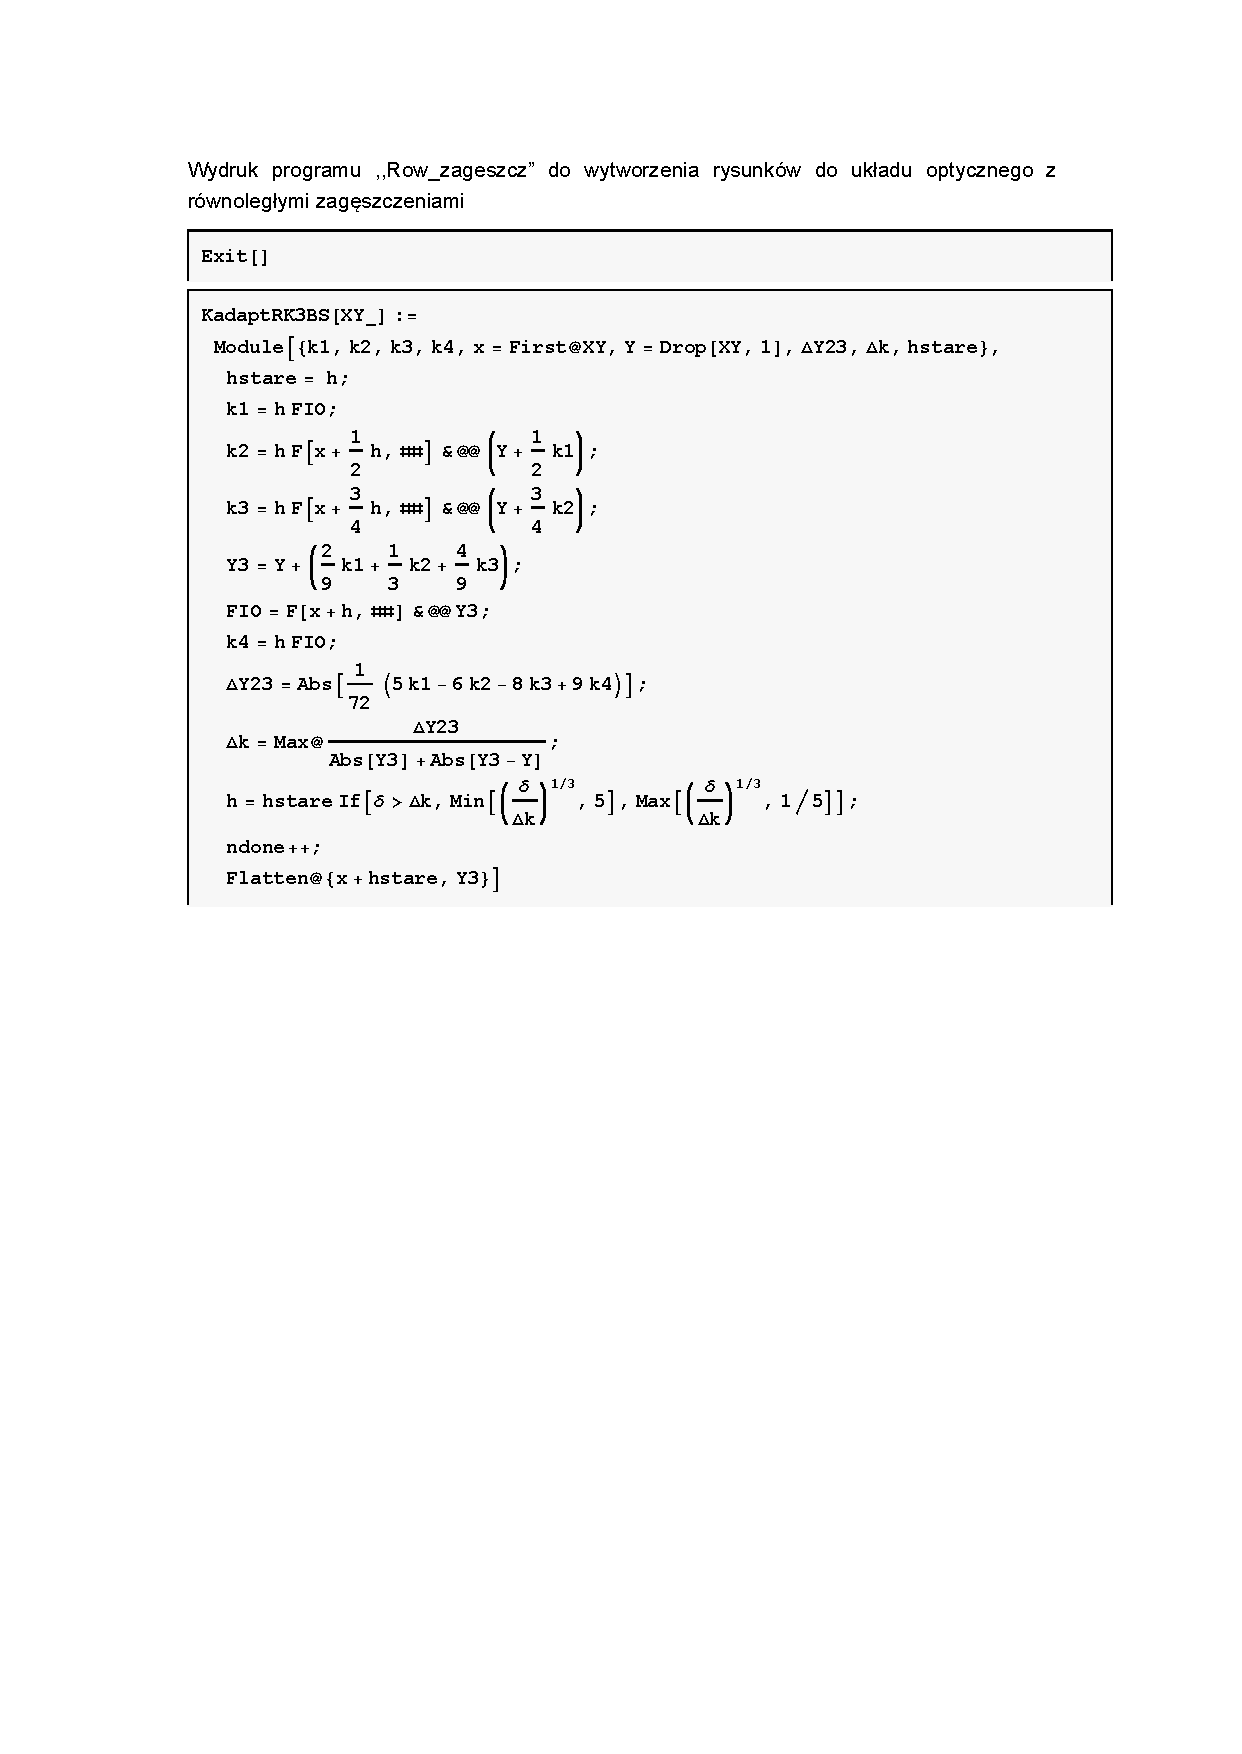
\includepdf[pages=-, scale=1]{grafika/Kod/Row_zageszcz.pdf}

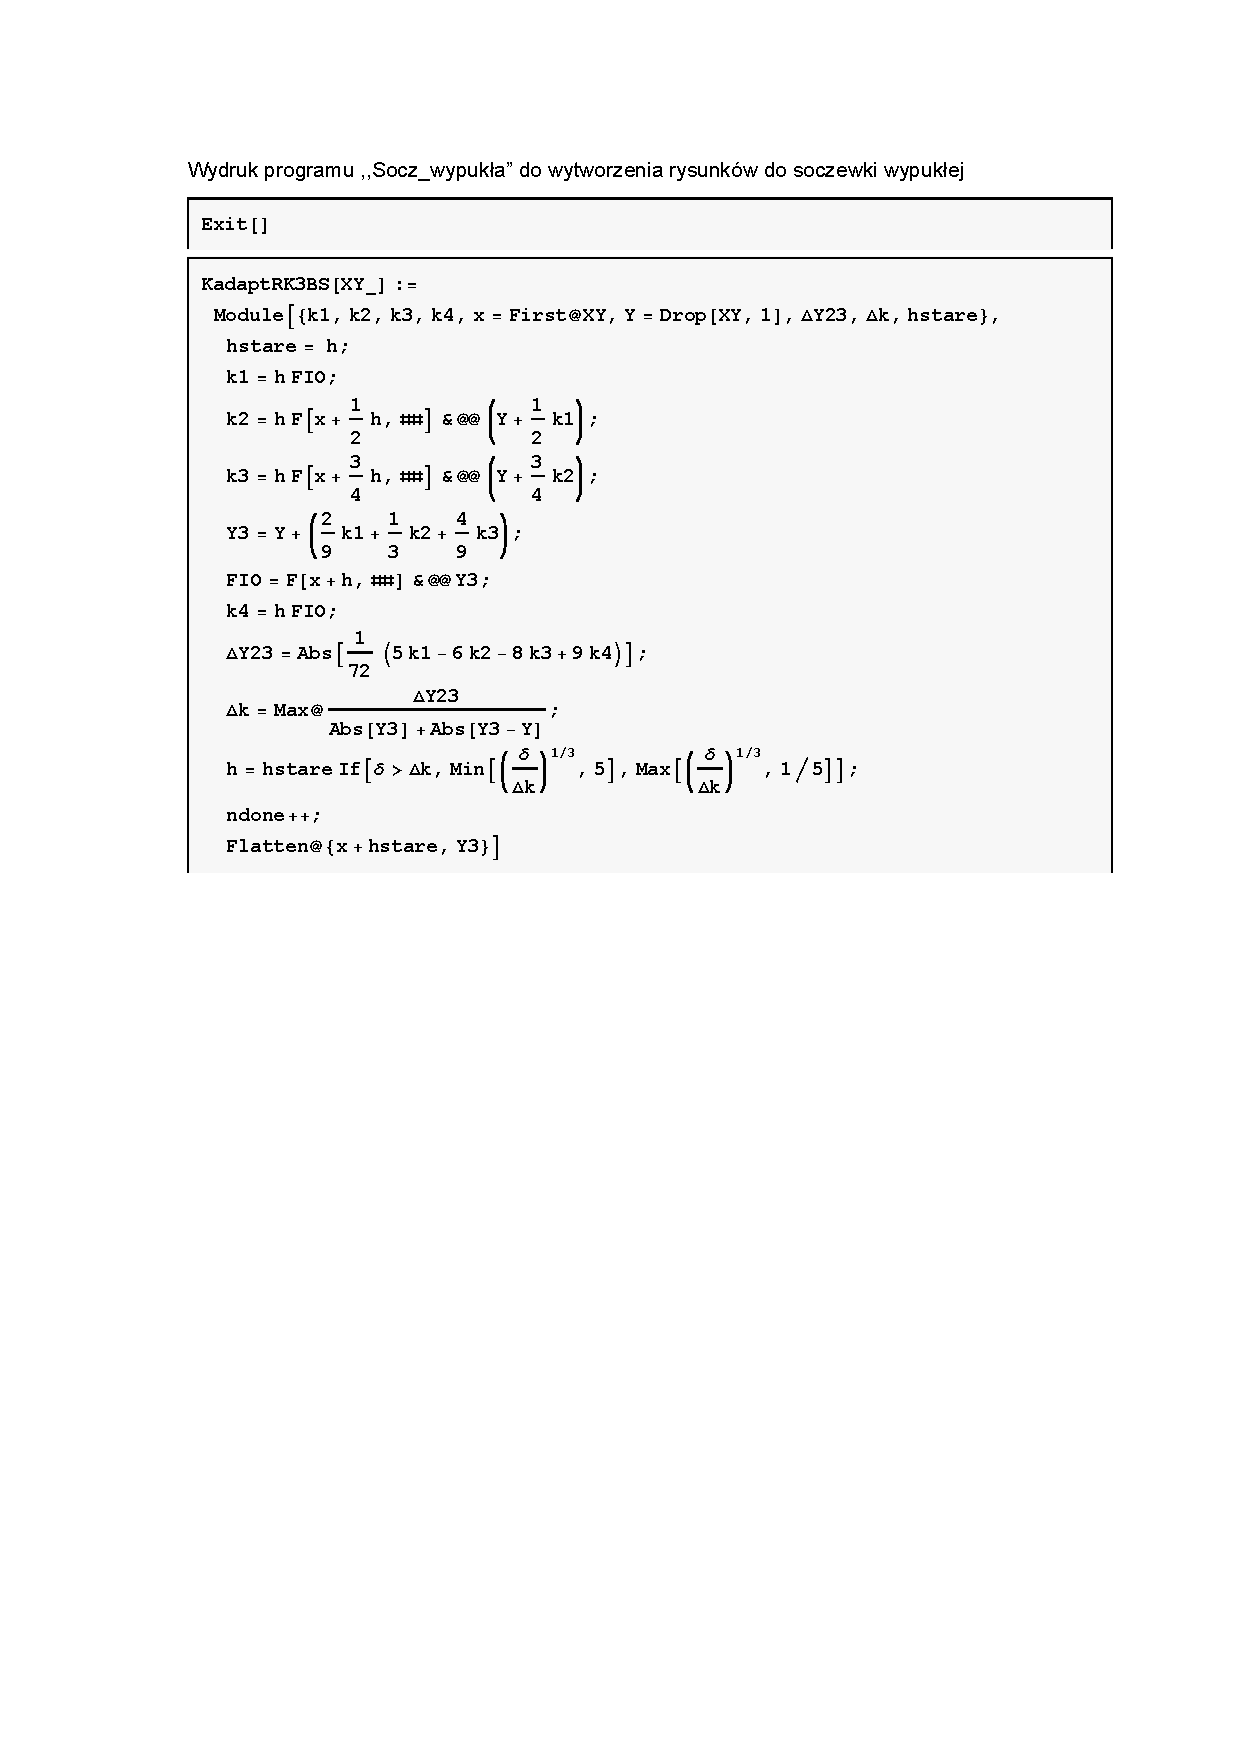
\includepdf[pages=-, scale=1]{grafika/Kod/Socz_wypukla.pdf}

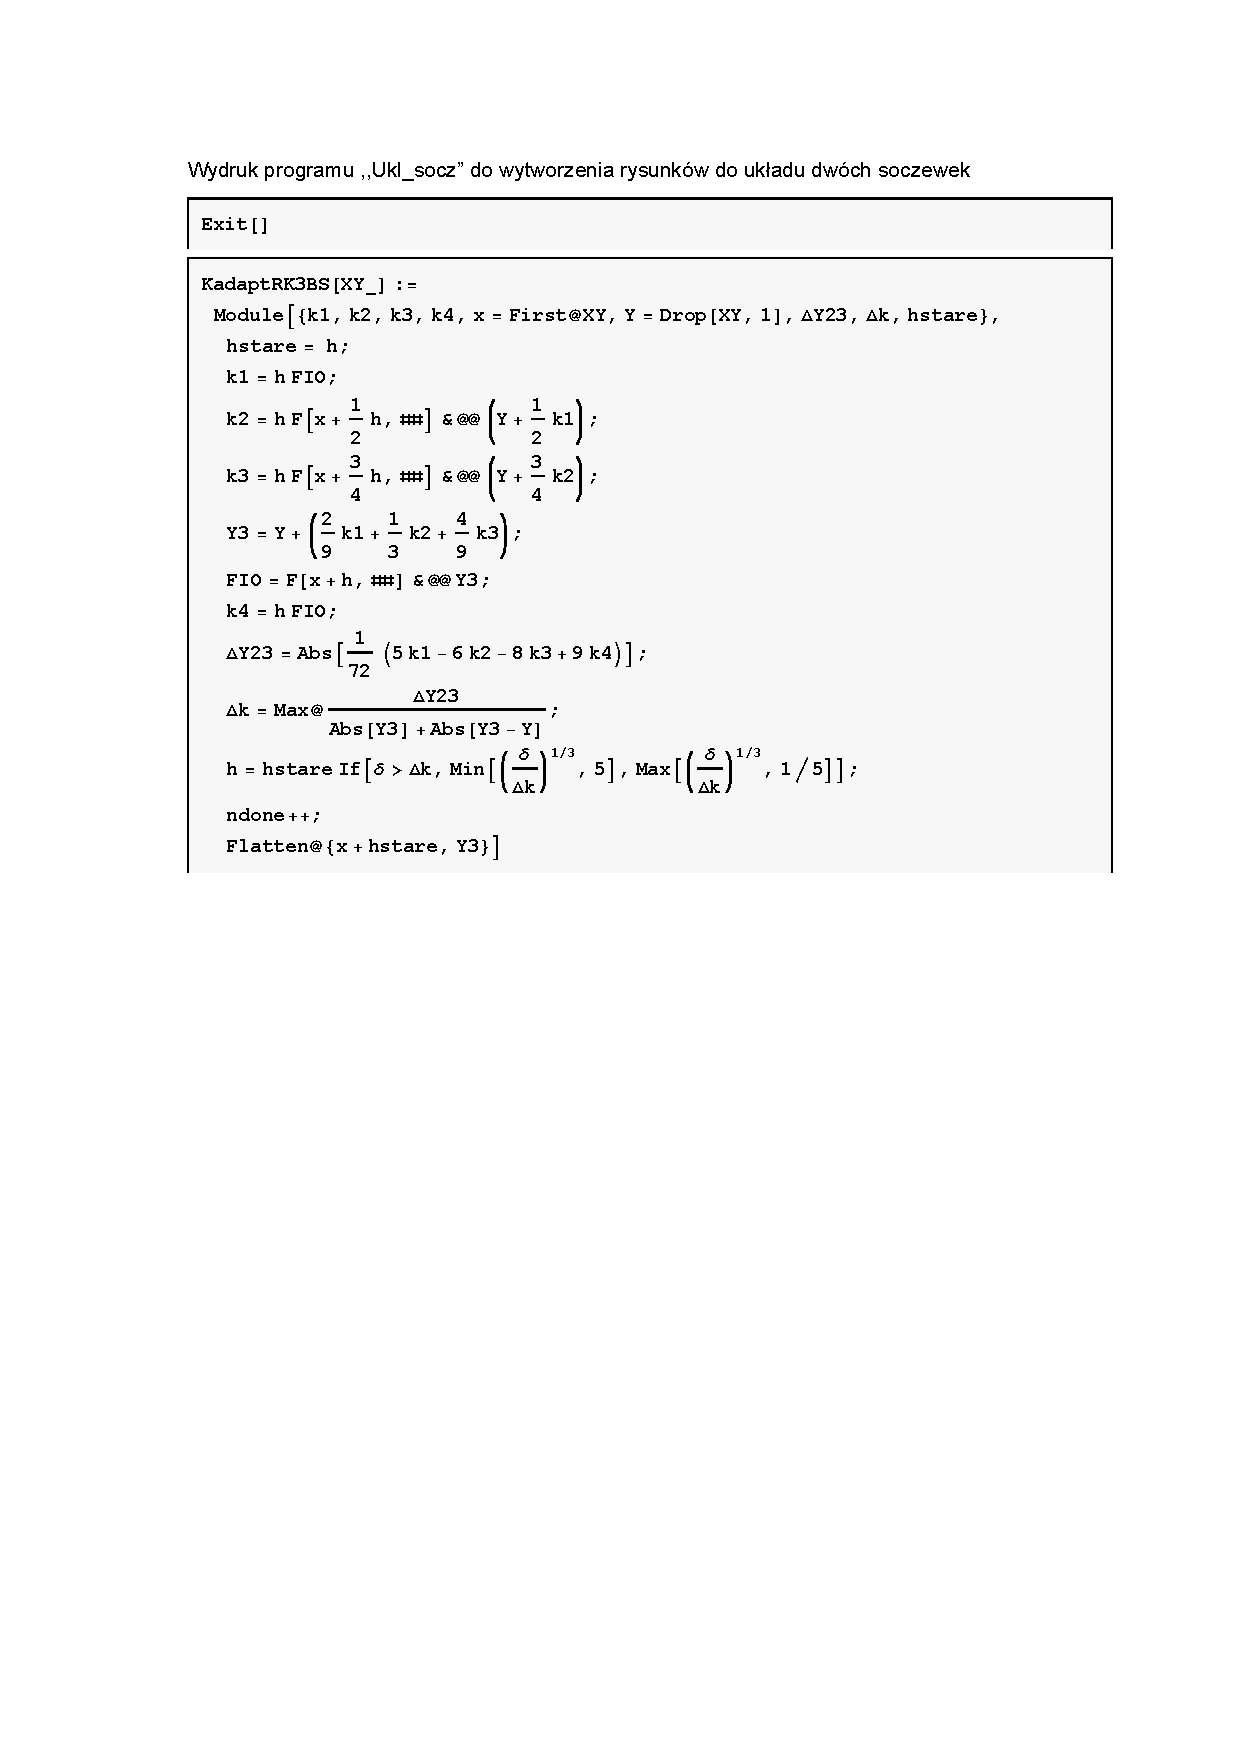
\includepdf[pages=-, scale=1]{grafika/Kod/Ukl_socz.pdf}

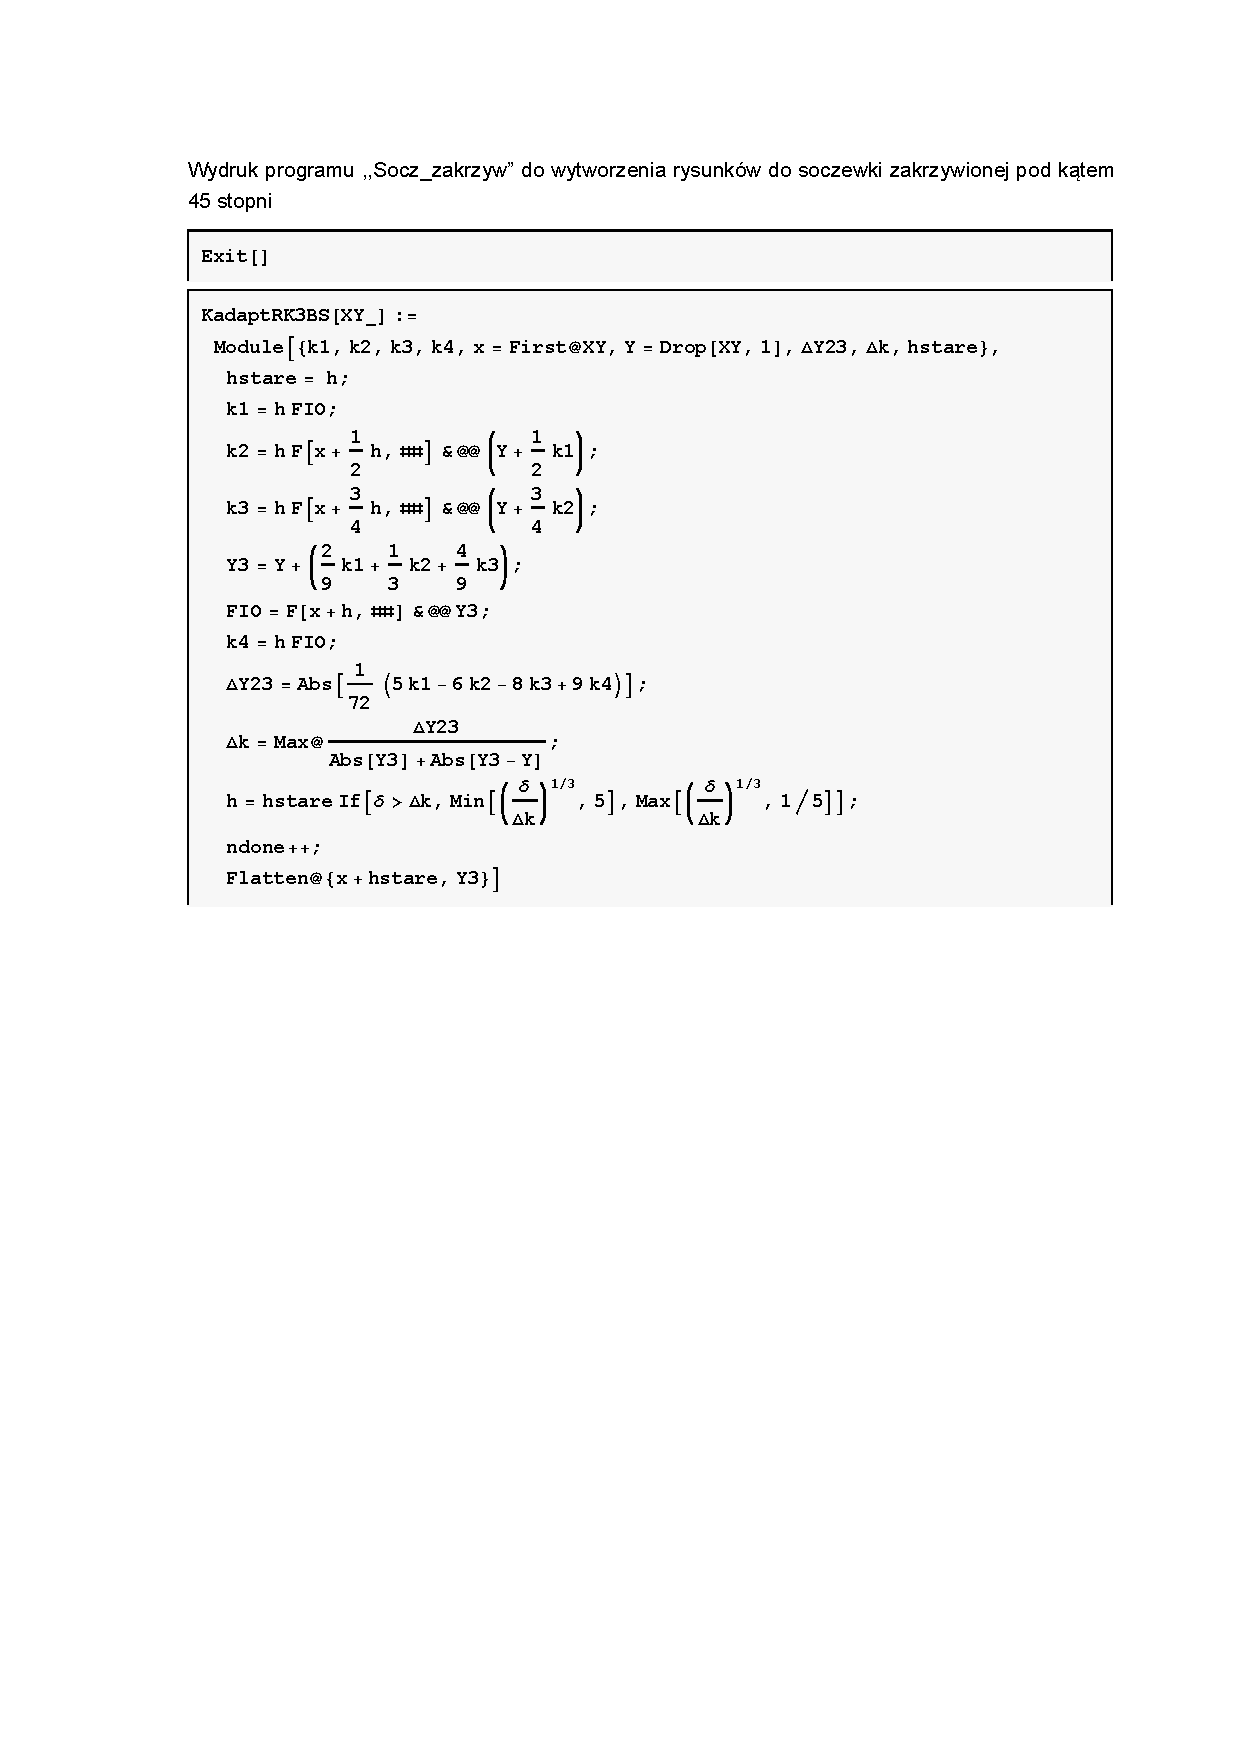
\includepdf[pages=-, scale=1]{grafika/Kod/Socz_zakrzyw.pdf}

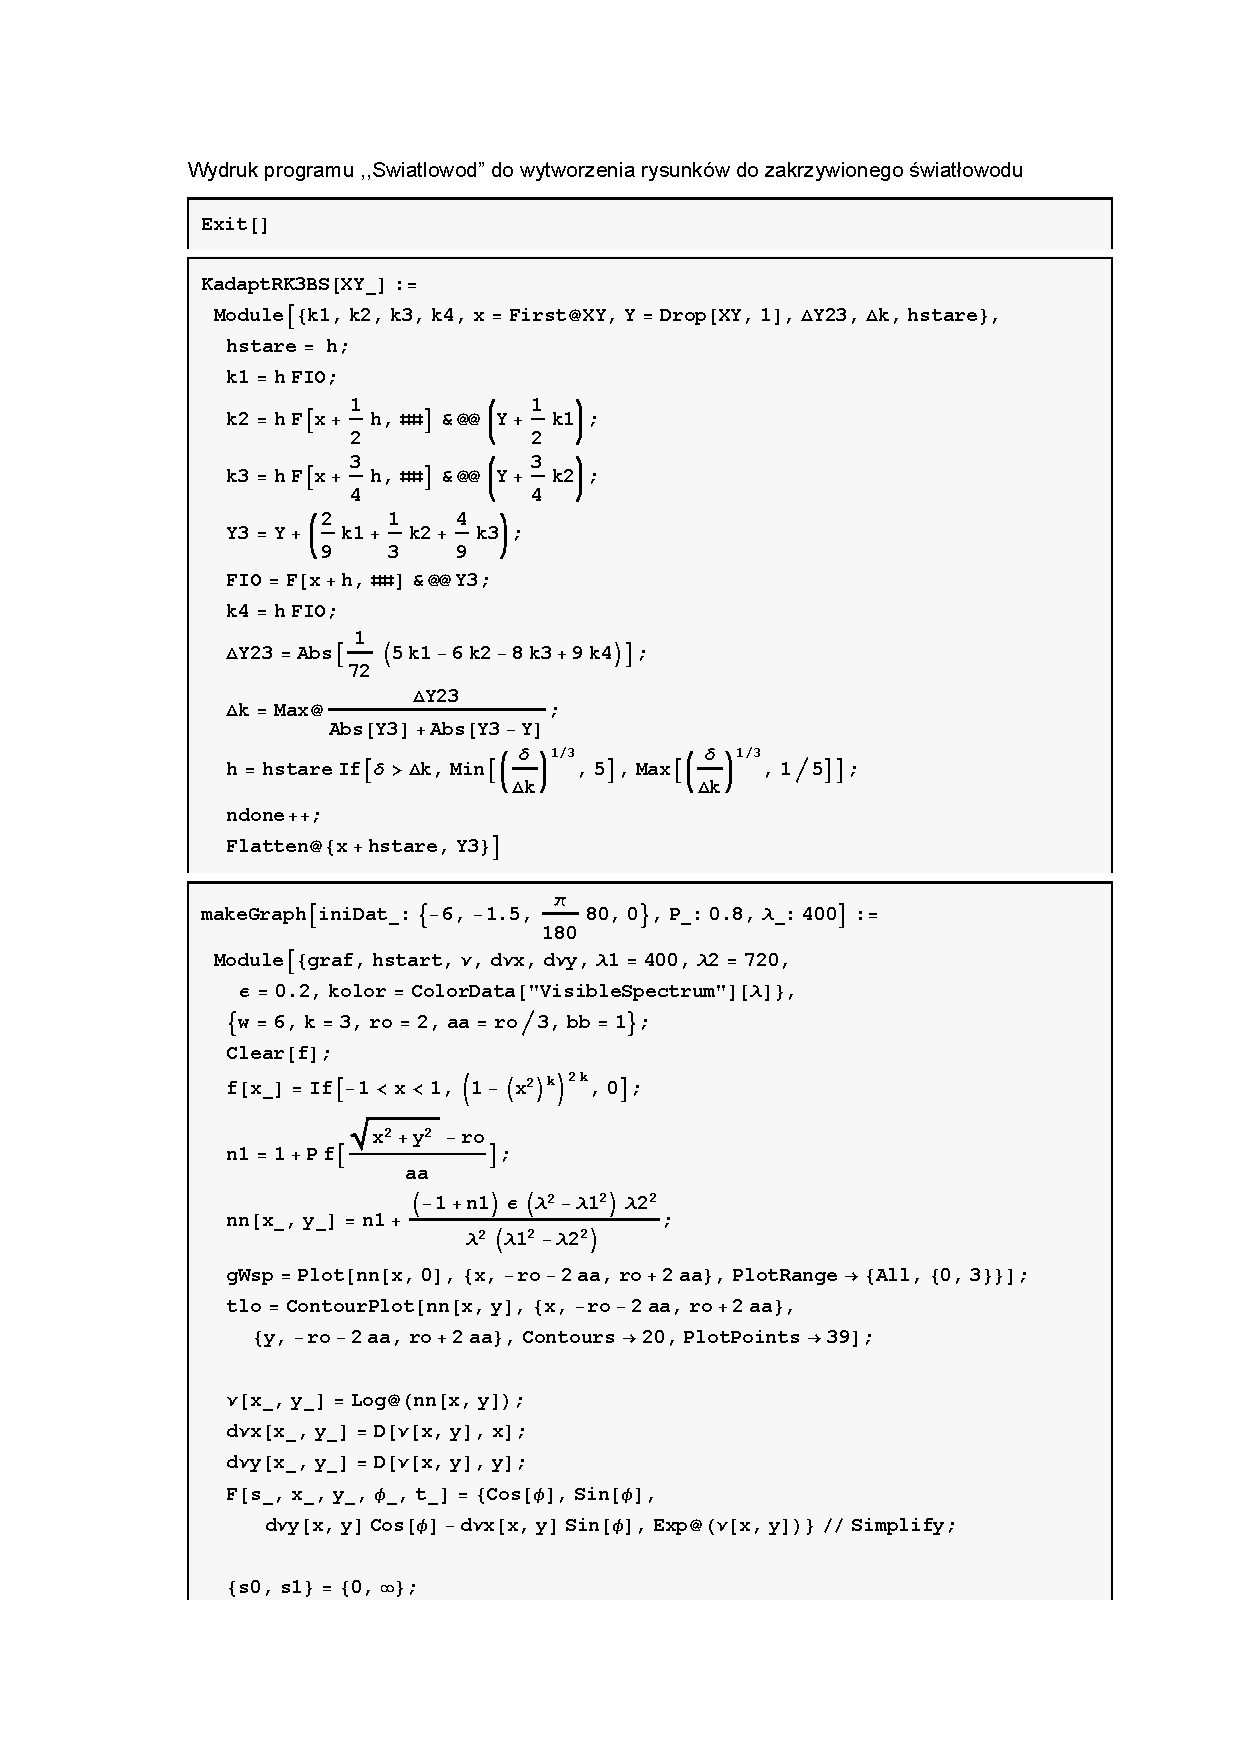
\includepdf[pages=-, scale=1]{grafika/Kod/Swiatlowod.pdf}

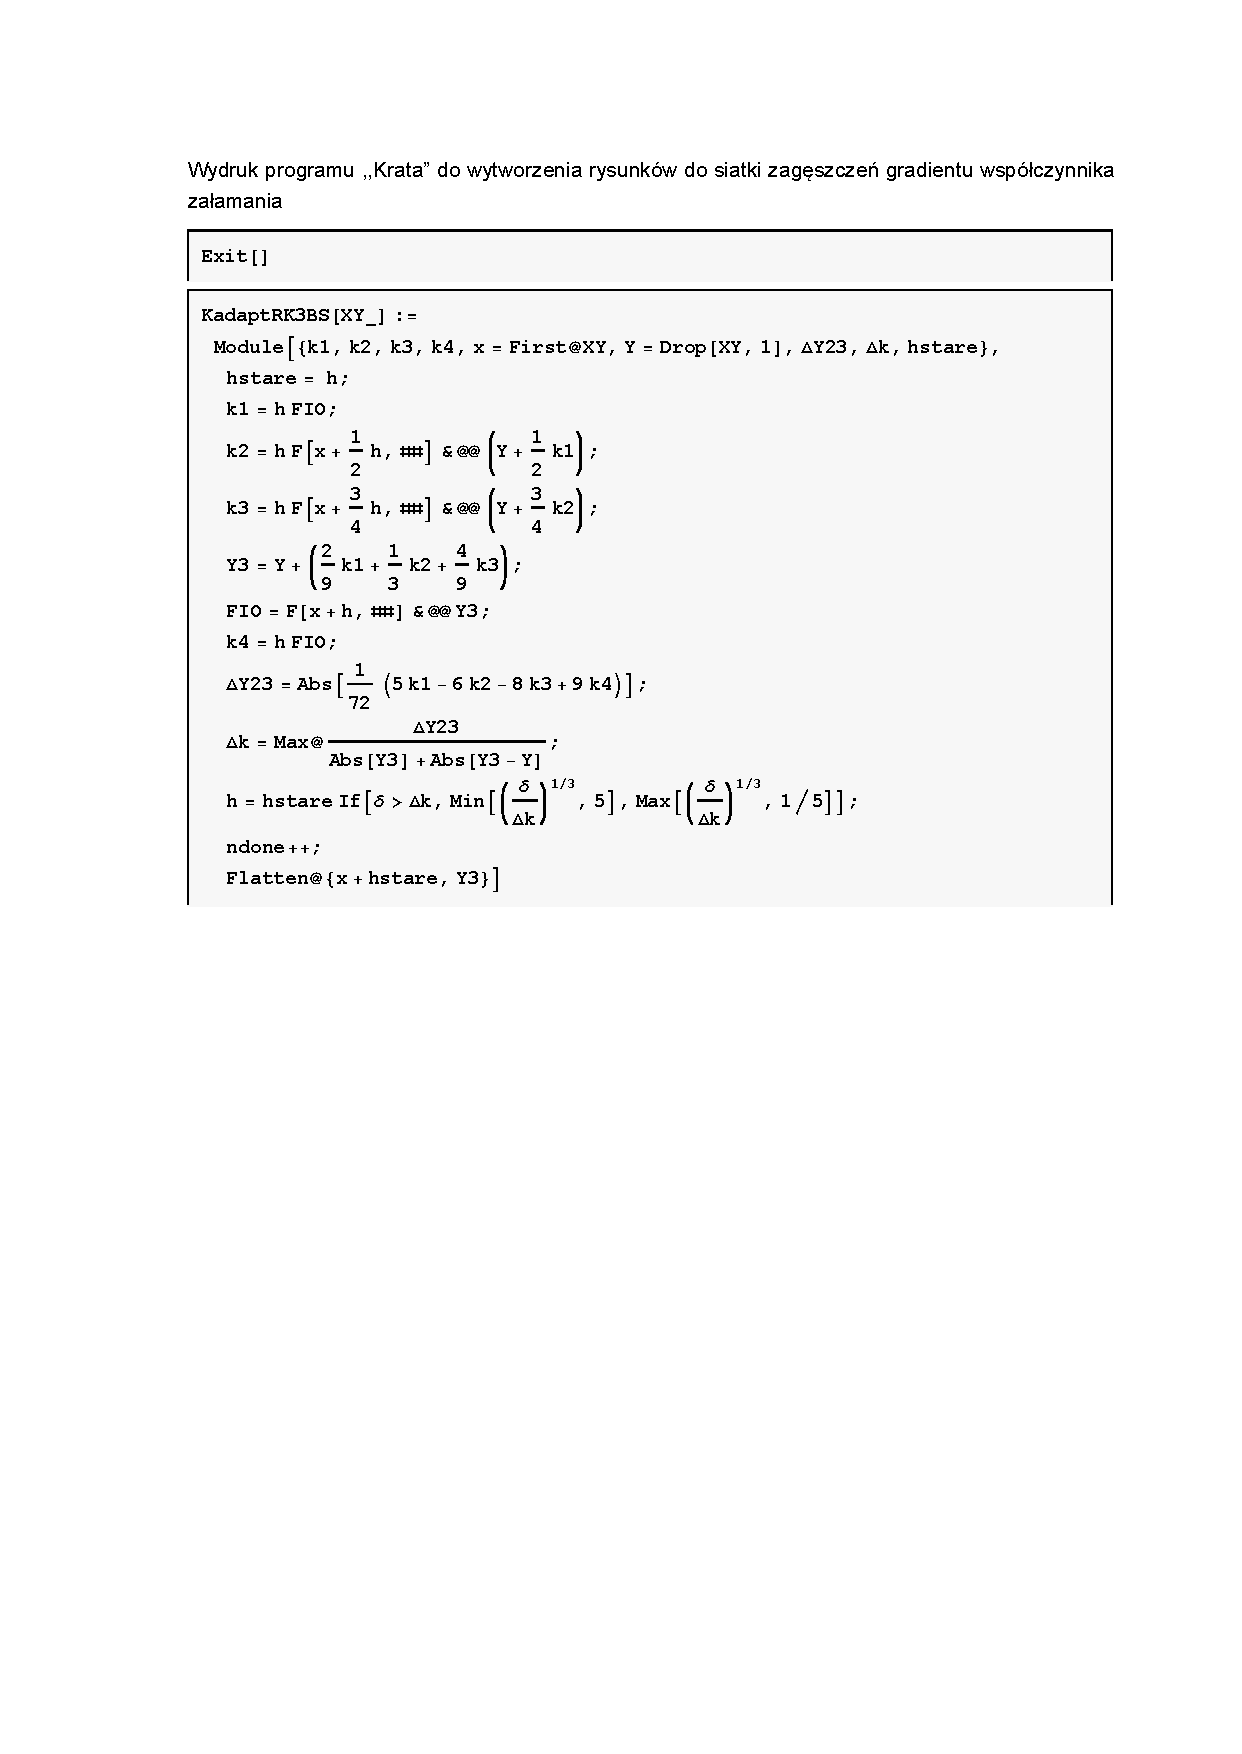
\includepdf[pages=-, scale=1]{grafika/Kod/Krata.pdf}

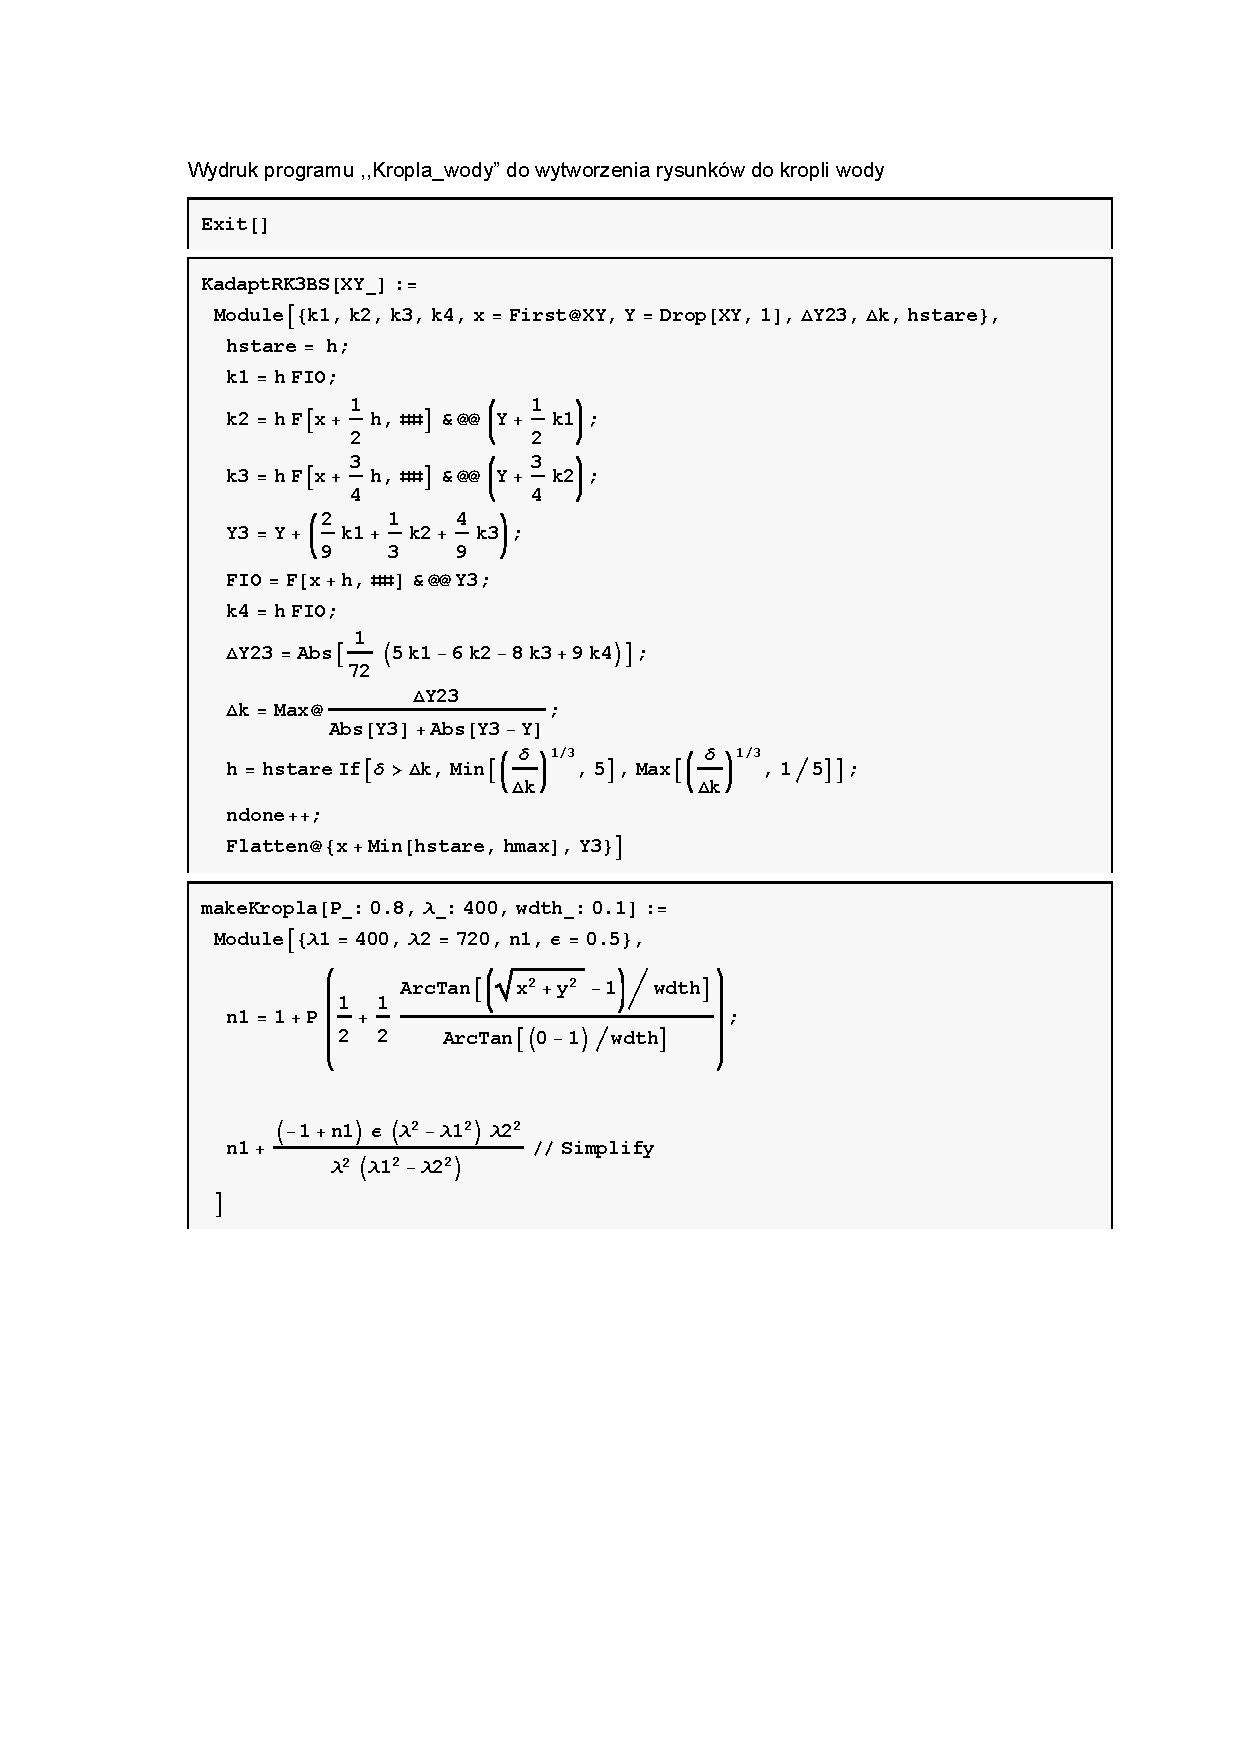
\includepdf[pages=-, scale=1]{grafika/Kod/Kropla_wody.pdf}

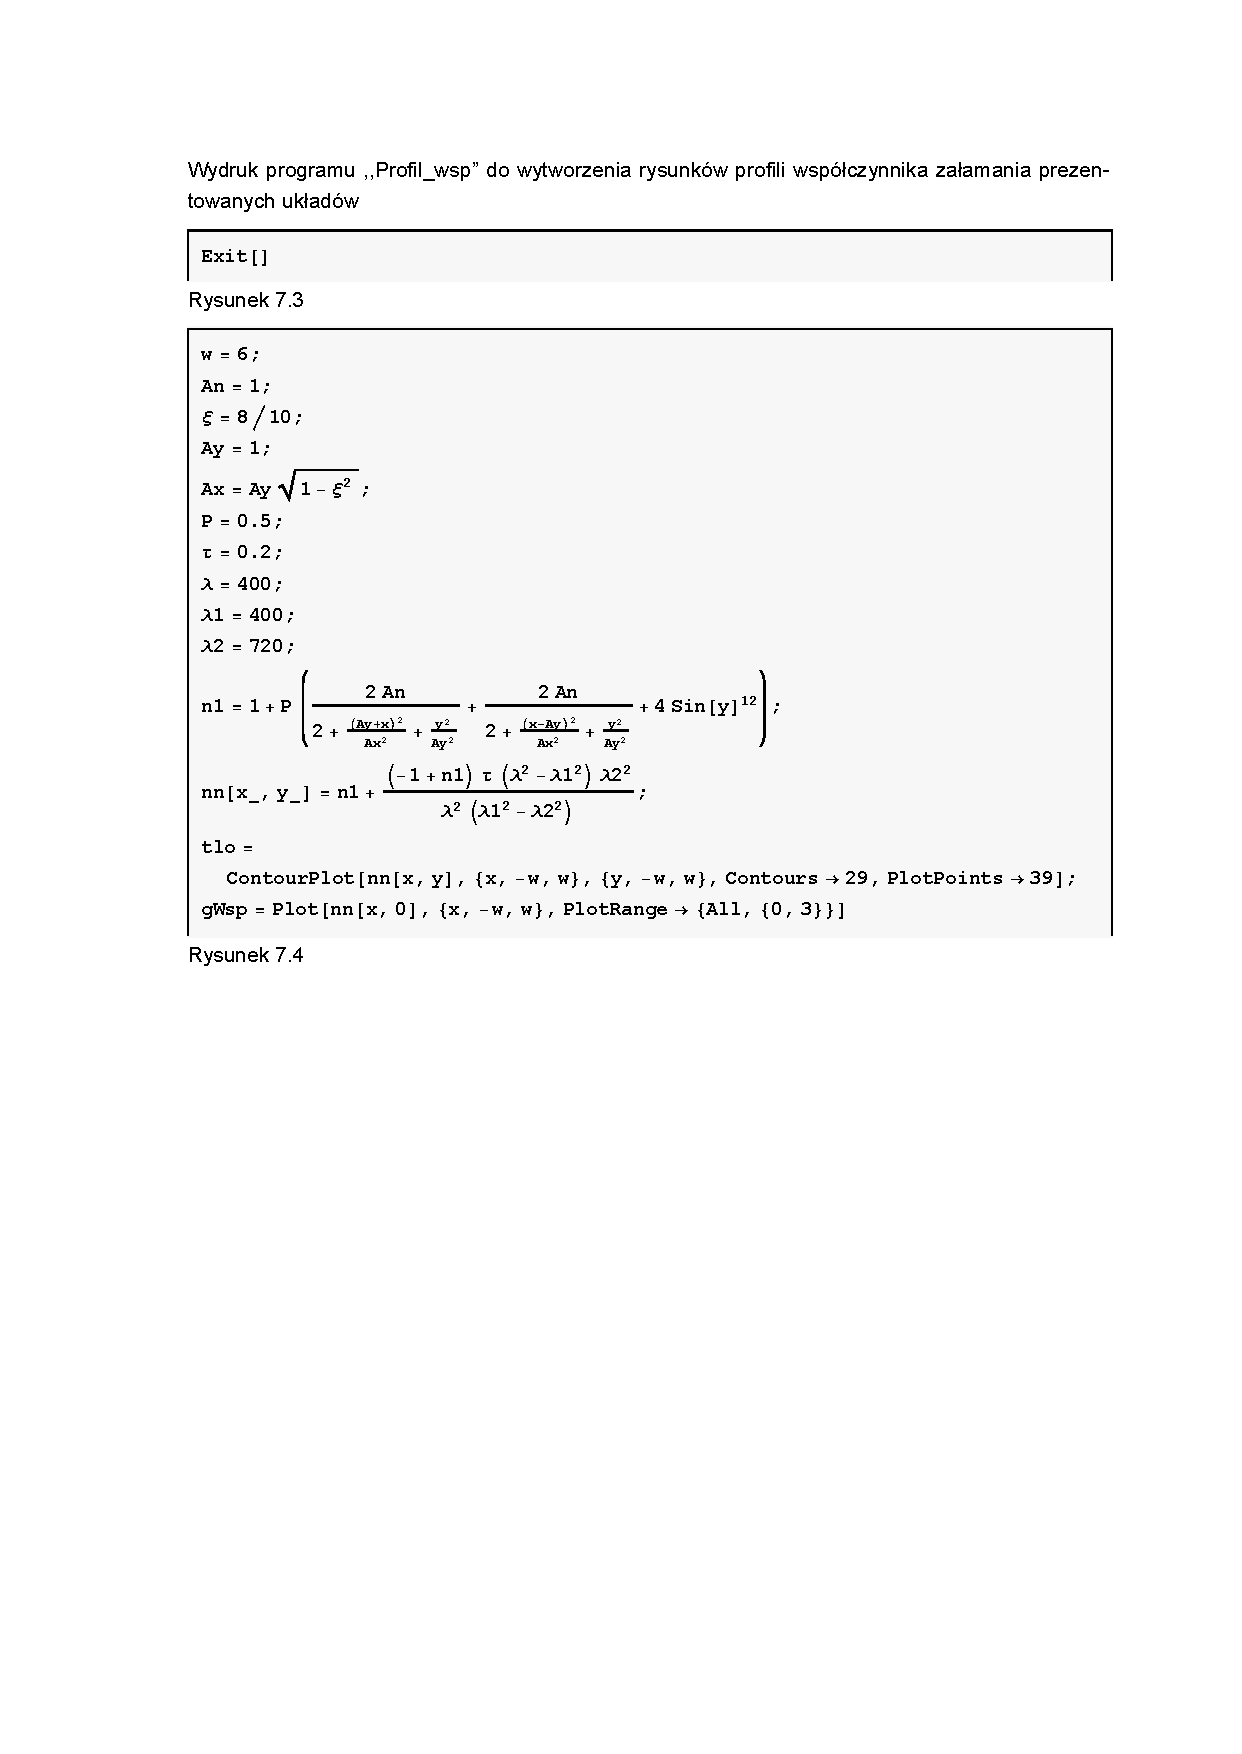
\includepdf[pages=-, scale=1]{grafika/Kod/Profil_wsp.pdf}

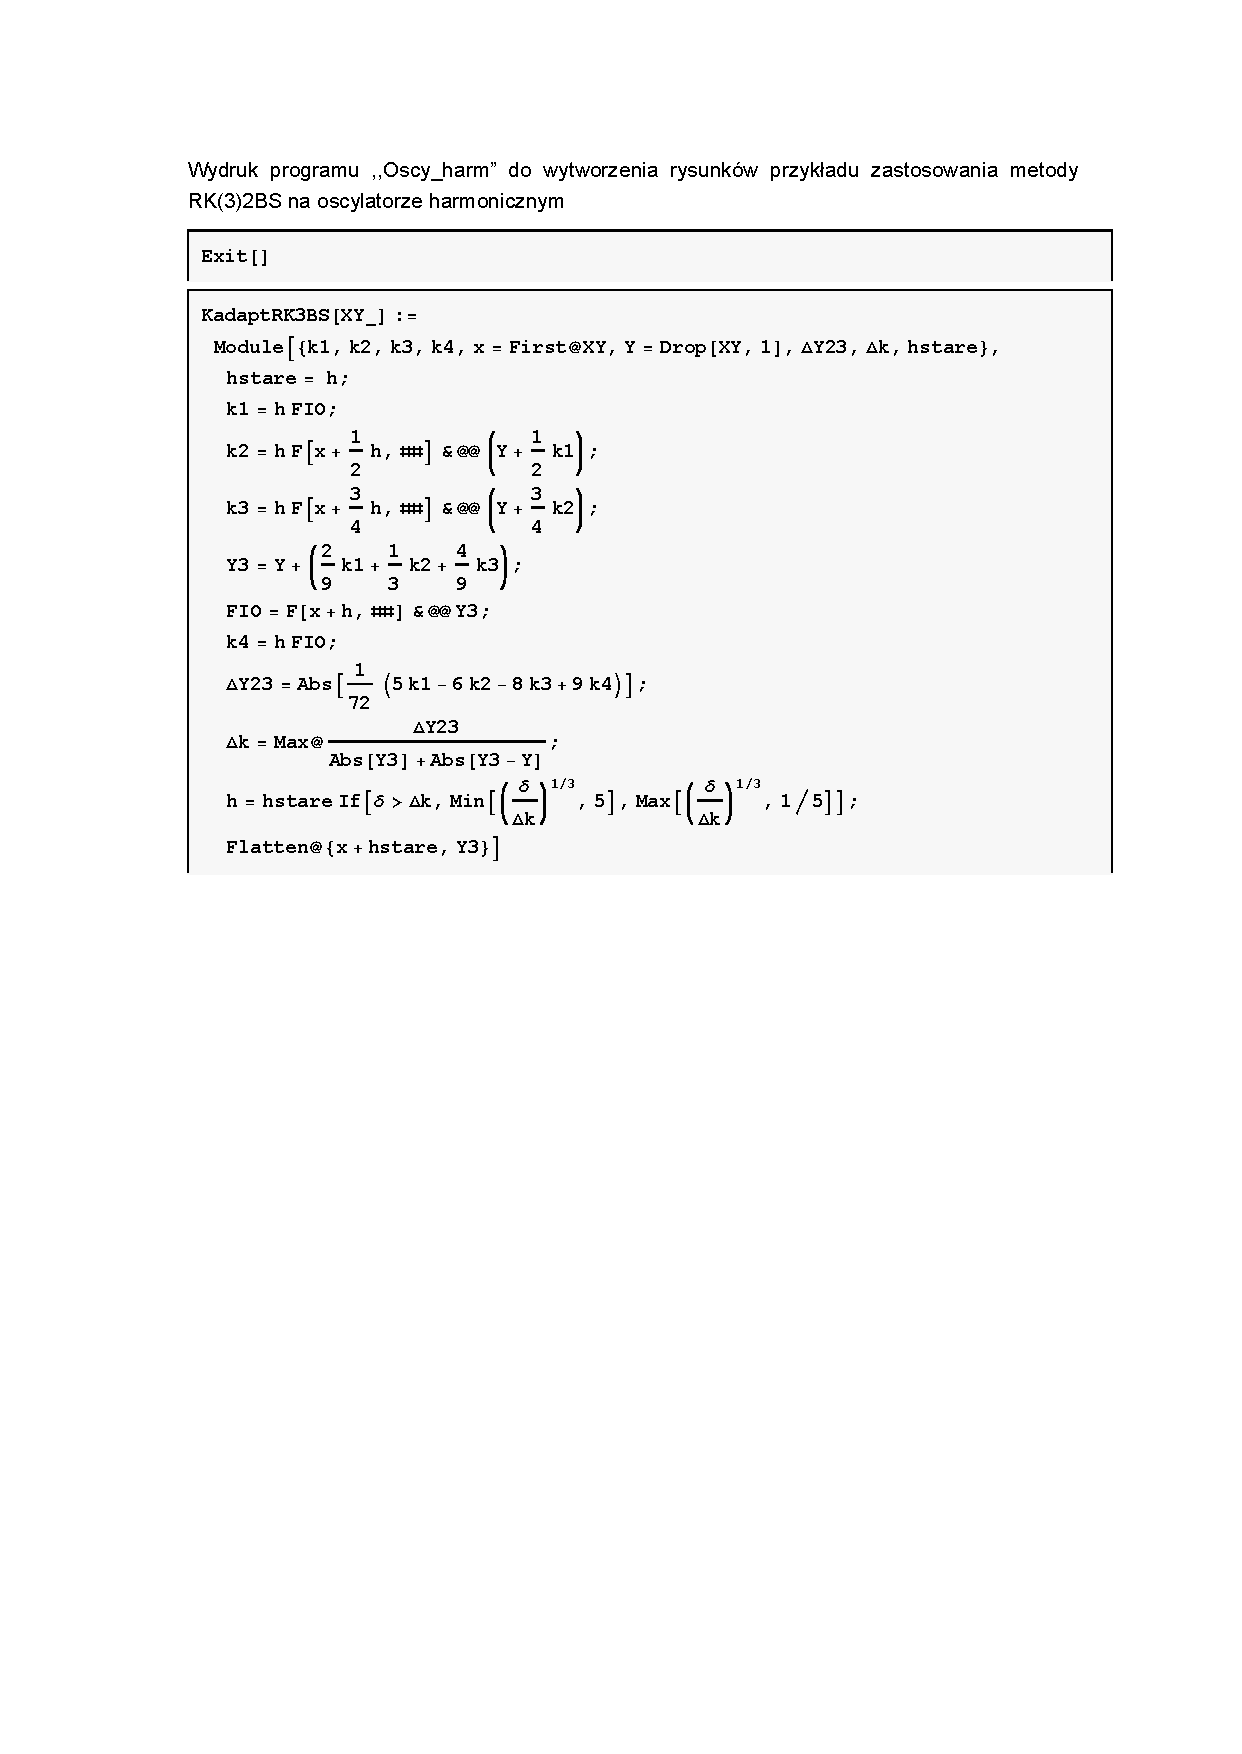
\includepdf[pages=-, scale=1]{grafika/Kod/Oscy_harm.pdf}

\end{document}